\documentclass[twoside]{book}

% Packages required by doxygen
\usepackage{fixltx2e}
\usepackage{calc}
\usepackage{doxygen}
\usepackage[export]{adjustbox} % also loads graphicx
\usepackage{graphicx}
\usepackage[utf8]{inputenc}
\usepackage{makeidx}
\usepackage{multicol}
\usepackage{multirow}
\PassOptionsToPackage{warn}{textcomp}
\usepackage{textcomp}
\usepackage[nointegrals]{wasysym}
\usepackage[table]{xcolor}

% Font selection
\usepackage[T1]{fontenc}
\usepackage[scaled=.90]{helvet}
\usepackage{courier}
\usepackage{amssymb}
\usepackage{sectsty}
\renewcommand{\familydefault}{\sfdefault}
\allsectionsfont{%
  \fontseries{bc}\selectfont%
  \color{darkgray}%
}
\renewcommand{\DoxyLabelFont}{%
  \fontseries{bc}\selectfont%
  \color{darkgray}%
}
\newcommand{\+}{\discretionary{\mbox{\scriptsize$\hookleftarrow$}}{}{}}

% Page & text layout
\usepackage{geometry}
\geometry{%
  a4paper,%
  top=2.5cm,%
  bottom=2.5cm,%
  left=2.5cm,%
  right=2.5cm%
}
\tolerance=750
\hfuzz=15pt
\hbadness=750
\setlength{\emergencystretch}{15pt}
\setlength{\parindent}{0cm}
\setlength{\parskip}{3ex plus 2ex minus 2ex}
\makeatletter
\renewcommand{\paragraph}{%
  \@startsection{paragraph}{4}{0ex}{-1.0ex}{1.0ex}{%
    \normalfont\normalsize\bfseries\SS@parafont%
  }%
}
\renewcommand{\subparagraph}{%
  \@startsection{subparagraph}{5}{0ex}{-1.0ex}{1.0ex}{%
    \normalfont\normalsize\bfseries\SS@subparafont%
  }%
}
\makeatother

% Headers & footers
\usepackage{fancyhdr}
\pagestyle{fancyplain}
\fancyhead[LE]{\fancyplain{}{\bfseries\thepage}}
\fancyhead[CE]{\fancyplain{}{}}
\fancyhead[RE]{\fancyplain{}{\bfseries\leftmark}}
\fancyhead[LO]{\fancyplain{}{\bfseries\rightmark}}
\fancyhead[CO]{\fancyplain{}{}}
\fancyhead[RO]{\fancyplain{}{\bfseries\thepage}}
\fancyfoot[LE]{\fancyplain{}{}}
\fancyfoot[CE]{\fancyplain{}{}}
\fancyfoot[RE]{\fancyplain{}{\bfseries\scriptsize Generated by Doxygen }}
\fancyfoot[LO]{\fancyplain{}{\bfseries\scriptsize Generated by Doxygen }}
\fancyfoot[CO]{\fancyplain{}{}}
\fancyfoot[RO]{\fancyplain{}{}}
\renewcommand{\footrulewidth}{0.4pt}
\renewcommand{\chaptermark}[1]{%
  \markboth{#1}{}%
}
\renewcommand{\sectionmark}[1]{%
  \markright{\thesection\ #1}%
}

% Indices & bibliography
\usepackage{natbib}
\usepackage[titles]{tocloft}
\setcounter{tocdepth}{3}
\setcounter{secnumdepth}{5}
\makeindex

% Hyperlinks (required, but should be loaded last)
\usepackage{ifpdf}
\ifpdf
  \usepackage[pdftex,pagebackref=true]{hyperref}
\else
  \usepackage[ps2pdf,pagebackref=true]{hyperref}
\fi
\hypersetup{%
  colorlinks=true,%
  linkcolor=blue,%
  citecolor=blue,%
  unicode%
}

% Custom commands
\newcommand{\clearemptydoublepage}{%
  \newpage{\pagestyle{empty}\cleardoublepage}%
}

\usepackage{caption}
\captionsetup{labelsep=space,justification=centering,font={bf},singlelinecheck=off,skip=4pt,position=top}

%===== C O N T E N T S =====

\begin{document}

% Titlepage & ToC
\hypersetup{pageanchor=false,
             bookmarksnumbered=true,
             pdfencoding=unicode
            }
\pagenumbering{alph}
\begin{titlepage}
\vspace*{7cm}
\begin{center}%
{\Large S\+F\+M\+L\+BE \\[1ex]\large 1.\+0 }\\
\vspace*{1cm}
{\large Generated by Doxygen 1.8.14}\\
\end{center}
\end{titlepage}
\clearemptydoublepage
\pagenumbering{roman}
\tableofcontents
\clearemptydoublepage
\pagenumbering{arabic}
\hypersetup{pageanchor=true}

%--- Begin generated contents ---
\chapter{S\+F\+M\+L\+BE}
\label{md__r_e_a_d_m_e}
\Hypertarget{md__r_e_a_d_m_e}
A simple and basic game engine for S\+F\+ML 2.\+0+ to gain time creating and managing a new game project 
\chapter{Namespace Index}
\section{Namespace List}
Here is a list of all documented namespaces with brief descriptions\+:\begin{DoxyCompactList}
\item\contentsline{section}{\mbox{\hyperlink{namespacesfmlbe}{sfmlbe}} }{\pageref{namespacesfmlbe}}{}
\end{DoxyCompactList}

\chapter{Hierarchical Index}
\section{Class Hierarchy}
This inheritance list is sorted roughly, but not completely, alphabetically\+:\begin{DoxyCompactList}
\item exception\begin{DoxyCompactList}
\item \contentsline{section}{sfmlbe\+:\+:Resource\+Not\+Found\+Exception}{\pageref{classsfmlbe_1_1_resource_not_found_exception}}{}
\item \contentsline{section}{sfmlbe\+:\+:Resource\+Not\+Load\+Exception}{\pageref{classsfmlbe_1_1_resource_not_load_exception}}{}
\item \contentsline{section}{sfmlbe\+:\+:Scope\+Not\+Found\+Exception}{\pageref{classsfmlbe_1_1_scope_not_found_exception}}{}
\end{DoxyCompactList}
\item \contentsline{section}{sfmlbe\+:\+:Resource}{\pageref{classsfmlbe_1_1_resource}}{}
\begin{DoxyCompactList}
\item \contentsline{section}{sfmlbe\+:\+:Resource\+Font}{\pageref{classsfmlbe_1_1_resource_font}}{}
\item \contentsline{section}{sfmlbe\+:\+:Resource\+Music}{\pageref{classsfmlbe_1_1_resource_music}}{}
\item \contentsline{section}{sfmlbe\+:\+:Resource\+Sound\+Buffer}{\pageref{classsfmlbe_1_1_resource_sound_buffer}}{}
\item \contentsline{section}{sfmlbe\+:\+:Resource\+Text}{\pageref{classsfmlbe_1_1_resource_text}}{}
\item \contentsline{section}{sfmlbe\+:\+:Resource\+Texture}{\pageref{classsfmlbe_1_1_resource_texture}}{}
\end{DoxyCompactList}
\item \contentsline{section}{sfmlbe\+:\+:Singleton$<$ T $>$}{\pageref{classsfmlbe_1_1_singleton}}{}
\item \contentsline{section}{sfmlbe\+:\+:Singleton$<$ Resource\+Manager $>$}{\pageref{classsfmlbe_1_1_singleton}}{}
\begin{DoxyCompactList}
\item \contentsline{section}{sfmlbe\+:\+:Resource\+Manager}{\pageref{classsfmlbe_1_1_resource_manager}}{}
\end{DoxyCompactList}
\end{DoxyCompactList}

\chapter{Class Index}
\section{Class List}
Here are the classes, structs, unions and interfaces with brief descriptions\+:\begin{DoxyCompactList}
\item\contentsline{section}{\mbox{\hyperlink{classsfmlbe_1_1_game_manager}{sfmlbe\+::\+Game\+Manager}} }{\pageref{classsfmlbe_1_1_game_manager}}{}
\item\contentsline{section}{\mbox{\hyperlink{structsfmlbe_1_1_game_parameters}{sfmlbe\+::\+Game\+Parameters}} }{\pageref{structsfmlbe_1_1_game_parameters}}{}
\item\contentsline{section}{\mbox{\hyperlink{classsfmlbe_1_1_game_state}{sfmlbe\+::\+Game\+State}} }{\pageref{classsfmlbe_1_1_game_state}}{}
\item\contentsline{section}{\mbox{\hyperlink{classsfmlbe_1_1_resource}{sfmlbe\+::\+Resource}} }{\pageref{classsfmlbe_1_1_resource}}{}
\item\contentsline{section}{\mbox{\hyperlink{classsfmlbe_1_1_resource_font}{sfmlbe\+::\+Resource\+Font}} }{\pageref{classsfmlbe_1_1_resource_font}}{}
\item\contentsline{section}{\mbox{\hyperlink{classsfmlbe_1_1_resource_manager}{sfmlbe\+::\+Resource\+Manager}} }{\pageref{classsfmlbe_1_1_resource_manager}}{}
\item\contentsline{section}{\mbox{\hyperlink{classsfmlbe_1_1_resource_music}{sfmlbe\+::\+Resource\+Music}} }{\pageref{classsfmlbe_1_1_resource_music}}{}
\item\contentsline{section}{\mbox{\hyperlink{classsfmlbe_1_1_resource_not_found_exception}{sfmlbe\+::\+Resource\+Not\+Found\+Exception}} }{\pageref{classsfmlbe_1_1_resource_not_found_exception}}{}
\item\contentsline{section}{\mbox{\hyperlink{classsfmlbe_1_1_resource_not_load_exception}{sfmlbe\+::\+Resource\+Not\+Load\+Exception}} }{\pageref{classsfmlbe_1_1_resource_not_load_exception}}{}
\item\contentsline{section}{\mbox{\hyperlink{classsfmlbe_1_1_resource_sound_buffer}{sfmlbe\+::\+Resource\+Sound\+Buffer}} }{\pageref{classsfmlbe_1_1_resource_sound_buffer}}{}
\item\contentsline{section}{\mbox{\hyperlink{classsfmlbe_1_1_resource_text}{sfmlbe\+::\+Resource\+Text}} }{\pageref{classsfmlbe_1_1_resource_text}}{}
\item\contentsline{section}{\mbox{\hyperlink{classsfmlbe_1_1_resource_texture}{sfmlbe\+::\+Resource\+Texture}} }{\pageref{classsfmlbe_1_1_resource_texture}}{}
\item\contentsline{section}{\mbox{\hyperlink{classsfmlbe_1_1_scope_not_found_exception}{sfmlbe\+::\+Scope\+Not\+Found\+Exception}} }{\pageref{classsfmlbe_1_1_scope_not_found_exception}}{}
\item\contentsline{section}{\mbox{\hyperlink{classsfmlbe_1_1_singleton}{sfmlbe\+::\+Singleton$<$ T $>$}} }{\pageref{classsfmlbe_1_1_singleton}}{}
\end{DoxyCompactList}

\chapter{File Index}
\section{File List}
Here is a list of all documented files with brief descriptions\+:\begin{DoxyCompactList}
\item\contentsline{section}{dev/header/\mbox{\hyperlink{common_8hpp}{common.\+hpp}} \\*Misc of component for S\+F\+M\+L\+BE }{\pageref{common_8hpp}}{}
\item\contentsline{section}{dev/header/\mbox{\hyperlink{resource_8hpp}{resource.\+hpp}} \\*Represent a resource }{\pageref{resource_8hpp}}{}
\item\contentsline{section}{dev/header/\mbox{\hyperlink{resourceexceptions_8hpp}{resourceexceptions.\+hpp}} \\*All the exceptions used in the Resource system }{\pageref{resourceexceptions_8hpp}}{}
\item\contentsline{section}{dev/header/\mbox{\hyperlink{resourcefont_8hpp}{resourcefont.\+hpp}} \\*Represent a resource storing a font }{\pageref{resourcefont_8hpp}}{}
\item\contentsline{section}{dev/header/\mbox{\hyperlink{resourcemanager_8hpp}{resourcemanager.\+hpp}} \\*Handle every resources loaded, accessible anywhere in the prgramme using Singleton pattern }{\pageref{resourcemanager_8hpp}}{}
\item\contentsline{section}{dev/header/\mbox{\hyperlink{resourcemusic_8hpp}{resourcemusic.\+hpp}} \\*Represent a resource storing a music }{\pageref{resourcemusic_8hpp}}{}
\item\contentsline{section}{dev/header/\mbox{\hyperlink{resourcesoundbuffer_8hpp}{resourcesoundbuffer.\+hpp}} \\*Represent a resource storing a soundbuffer }{\pageref{resourcesoundbuffer_8hpp}}{}
\item\contentsline{section}{dev/header/\mbox{\hyperlink{resourcetext_8hpp}{resourcetext.\+hpp}} \\*Represent a resource storing texts }{\pageref{resourcetext_8hpp}}{}
\item\contentsline{section}{dev/header/\mbox{\hyperlink{resourcetexture_8hpp}{resourcetexture.\+hpp}} \\*Represent a resource storing a texture }{\pageref{resourcetexture_8hpp}}{}
\item\contentsline{section}{dev/header/\mbox{\hyperlink{singleton_8hpp}{singleton.\+hpp}} \\*Template for a Singleton, based on this tutorial \+: \href{https://come-david.developpez.com/tutoriels/dps/?page=Singleton}{\tt https\+://come-\/david.\+developpez.\+com/tutoriels/dps/?page=\+Singleton} }{\pageref{singleton_8hpp}}{}
\end{DoxyCompactList}

\chapter{Namespace Documentation}
\hypertarget{namespacesfmlbe}{}\section{sfmlbe Namespace Reference}
\label{namespacesfmlbe}\index{sfmlbe@{sfmlbe}}
\subsection*{Classes}
\begin{DoxyCompactItemize}
\item 
class \mbox{\hyperlink{classsfmlbe_1_1_resource}{Resource}}
\item 
class \mbox{\hyperlink{classsfmlbe_1_1_resource_font}{Resource\+Font}}
\item 
class \mbox{\hyperlink{classsfmlbe_1_1_resource_manager}{Resource\+Manager}}
\item 
class \mbox{\hyperlink{classsfmlbe_1_1_resource_music}{Resource\+Music}}
\item 
class \mbox{\hyperlink{classsfmlbe_1_1_resource_not_found_exception}{Resource\+Not\+Found\+Exception}}
\item 
class \mbox{\hyperlink{classsfmlbe_1_1_resource_not_load_exception}{Resource\+Not\+Load\+Exception}}
\item 
class \mbox{\hyperlink{classsfmlbe_1_1_resource_sound_buffer}{Resource\+Sound\+Buffer}}
\item 
class \mbox{\hyperlink{classsfmlbe_1_1_resource_text}{Resource\+Text}}
\item 
class \mbox{\hyperlink{classsfmlbe_1_1_resource_texture}{Resource\+Texture}}
\item 
class \mbox{\hyperlink{classsfmlbe_1_1_scope_not_found_exception}{Scope\+Not\+Found\+Exception}}
\item 
class \mbox{\hyperlink{classsfmlbe_1_1_singleton}{Singleton}}
\end{DoxyCompactItemize}
\subsection*{Enumerations}
\begin{DoxyCompactItemize}
\item 
enum \mbox{\hyperlink{namespacesfmlbe_ac4335ed3060bba025f73e01f9dccb2dd}{R\+E\+S\+O\+U\+R\+C\+E\+\_\+\+T\+Y\+PE}} \{ \newline
\mbox{\hyperlink{namespacesfmlbe_ac4335ed3060bba025f73e01f9dccb2dda8d19259bccf0ab6ee075b32fff6f7e54}{R\+E\+S\+O\+U\+R\+C\+E\+\_\+\+N\+U\+LL}} = 0, 
\mbox{\hyperlink{namespacesfmlbe_ac4335ed3060bba025f73e01f9dccb2dda660c8cdfebf28528f6f0631ae29f89a5}{R\+E\+S\+O\+U\+R\+C\+E\+\_\+\+G\+R\+A\+P\+H\+IC}} = 1, 
\mbox{\hyperlink{namespacesfmlbe_ac4335ed3060bba025f73e01f9dccb2dda06cb8047cf98a2679b83166ad27d2708}{R\+E\+S\+O\+U\+R\+C\+E\+\_\+\+S\+O\+U\+N\+D\+B\+U\+F\+F\+ER}} = 2, 
\mbox{\hyperlink{namespacesfmlbe_ac4335ed3060bba025f73e01f9dccb2ddab44bcfdfdfd1fd38857b8ad914608007}{R\+E\+S\+O\+U\+R\+C\+E\+\_\+\+M\+U\+S\+IC}} = 3, 
\newline
\mbox{\hyperlink{namespacesfmlbe_ac4335ed3060bba025f73e01f9dccb2dda9550a304907119d426805e6ed9a6c193}{R\+E\+S\+O\+U\+R\+C\+E\+\_\+\+T\+E\+XT}} = 4, 
\mbox{\hyperlink{namespacesfmlbe_ac4335ed3060bba025f73e01f9dccb2dda7eae53eb53c90d3adcdfa9a16ebc34b7}{R\+E\+S\+O\+U\+R\+C\+E\+\_\+\+F\+O\+NT}} = 5
 \}
\end{DoxyCompactItemize}


\subsection{Detailed Description}
Namespace for this engine. 

\subsection{Enumeration Type Documentation}
\mbox{\Hypertarget{namespacesfmlbe_ac4335ed3060bba025f73e01f9dccb2dd}\label{namespacesfmlbe_ac4335ed3060bba025f73e01f9dccb2dd}} 
\index{sfmlbe@{sfmlbe}!R\+E\+S\+O\+U\+R\+C\+E\+\_\+\+T\+Y\+PE@{R\+E\+S\+O\+U\+R\+C\+E\+\_\+\+T\+Y\+PE}}
\index{R\+E\+S\+O\+U\+R\+C\+E\+\_\+\+T\+Y\+PE@{R\+E\+S\+O\+U\+R\+C\+E\+\_\+\+T\+Y\+PE}!sfmlbe@{sfmlbe}}
\subsubsection{\texorpdfstring{R\+E\+S\+O\+U\+R\+C\+E\+\_\+\+T\+Y\+PE}{RESOURCE\_TYPE}}
{\footnotesize\ttfamily enum \mbox{\hyperlink{namespacesfmlbe_ac4335ed3060bba025f73e01f9dccb2dd}{sfmlbe\+::\+R\+E\+S\+O\+U\+R\+C\+E\+\_\+\+T\+Y\+PE}}}

Enum defining every type of resource possible. \begin{DoxyEnumFields}{Enumerator}
\raisebox{\heightof{T}}[0pt][0pt]{\index{R\+E\+S\+O\+U\+R\+C\+E\+\_\+\+N\+U\+LL@{R\+E\+S\+O\+U\+R\+C\+E\+\_\+\+N\+U\+LL}!sfmlbe@{sfmlbe}}\index{sfmlbe@{sfmlbe}!R\+E\+S\+O\+U\+R\+C\+E\+\_\+\+N\+U\+LL@{R\+E\+S\+O\+U\+R\+C\+E\+\_\+\+N\+U\+LL}}}\mbox{\Hypertarget{namespacesfmlbe_ac4335ed3060bba025f73e01f9dccb2dda8d19259bccf0ab6ee075b32fff6f7e54}\label{namespacesfmlbe_ac4335ed3060bba025f73e01f9dccb2dda8d19259bccf0ab6ee075b32fff6f7e54}} 
R\+E\+S\+O\+U\+R\+C\+E\+\_\+\+N\+U\+LL&Represent a not valid resource. \\
\hline

\raisebox{\heightof{T}}[0pt][0pt]{\index{R\+E\+S\+O\+U\+R\+C\+E\+\_\+\+G\+R\+A\+P\+H\+IC@{R\+E\+S\+O\+U\+R\+C\+E\+\_\+\+G\+R\+A\+P\+H\+IC}!sfmlbe@{sfmlbe}}\index{sfmlbe@{sfmlbe}!R\+E\+S\+O\+U\+R\+C\+E\+\_\+\+G\+R\+A\+P\+H\+IC@{R\+E\+S\+O\+U\+R\+C\+E\+\_\+\+G\+R\+A\+P\+H\+IC}}}\mbox{\Hypertarget{namespacesfmlbe_ac4335ed3060bba025f73e01f9dccb2dda660c8cdfebf28528f6f0631ae29f89a5}\label{namespacesfmlbe_ac4335ed3060bba025f73e01f9dccb2dda660c8cdfebf28528f6f0631ae29f89a5}} 
R\+E\+S\+O\+U\+R\+C\+E\+\_\+\+G\+R\+A\+P\+H\+IC&Represent a texture resource. \\
\hline

\raisebox{\heightof{T}}[0pt][0pt]{\index{R\+E\+S\+O\+U\+R\+C\+E\+\_\+\+S\+O\+U\+N\+D\+B\+U\+F\+F\+ER@{R\+E\+S\+O\+U\+R\+C\+E\+\_\+\+S\+O\+U\+N\+D\+B\+U\+F\+F\+ER}!sfmlbe@{sfmlbe}}\index{sfmlbe@{sfmlbe}!R\+E\+S\+O\+U\+R\+C\+E\+\_\+\+S\+O\+U\+N\+D\+B\+U\+F\+F\+ER@{R\+E\+S\+O\+U\+R\+C\+E\+\_\+\+S\+O\+U\+N\+D\+B\+U\+F\+F\+ER}}}\mbox{\Hypertarget{namespacesfmlbe_ac4335ed3060bba025f73e01f9dccb2dda06cb8047cf98a2679b83166ad27d2708}\label{namespacesfmlbe_ac4335ed3060bba025f73e01f9dccb2dda06cb8047cf98a2679b83166ad27d2708}} 
R\+E\+S\+O\+U\+R\+C\+E\+\_\+\+S\+O\+U\+N\+D\+B\+U\+F\+F\+ER&Represent a soundbuffer resource. \\
\hline

\raisebox{\heightof{T}}[0pt][0pt]{\index{R\+E\+S\+O\+U\+R\+C\+E\+\_\+\+M\+U\+S\+IC@{R\+E\+S\+O\+U\+R\+C\+E\+\_\+\+M\+U\+S\+IC}!sfmlbe@{sfmlbe}}\index{sfmlbe@{sfmlbe}!R\+E\+S\+O\+U\+R\+C\+E\+\_\+\+M\+U\+S\+IC@{R\+E\+S\+O\+U\+R\+C\+E\+\_\+\+M\+U\+S\+IC}}}\mbox{\Hypertarget{namespacesfmlbe_ac4335ed3060bba025f73e01f9dccb2ddab44bcfdfdfd1fd38857b8ad914608007}\label{namespacesfmlbe_ac4335ed3060bba025f73e01f9dccb2ddab44bcfdfdfd1fd38857b8ad914608007}} 
R\+E\+S\+O\+U\+R\+C\+E\+\_\+\+M\+U\+S\+IC&Represent a music resource. \\
\hline

\raisebox{\heightof{T}}[0pt][0pt]{\index{R\+E\+S\+O\+U\+R\+C\+E\+\_\+\+T\+E\+XT@{R\+E\+S\+O\+U\+R\+C\+E\+\_\+\+T\+E\+XT}!sfmlbe@{sfmlbe}}\index{sfmlbe@{sfmlbe}!R\+E\+S\+O\+U\+R\+C\+E\+\_\+\+T\+E\+XT@{R\+E\+S\+O\+U\+R\+C\+E\+\_\+\+T\+E\+XT}}}\mbox{\Hypertarget{namespacesfmlbe_ac4335ed3060bba025f73e01f9dccb2dda9550a304907119d426805e6ed9a6c193}\label{namespacesfmlbe_ac4335ed3060bba025f73e01f9dccb2dda9550a304907119d426805e6ed9a6c193}} 
R\+E\+S\+O\+U\+R\+C\+E\+\_\+\+T\+E\+XT&Represent a string resource. \\
\hline

\raisebox{\heightof{T}}[0pt][0pt]{\index{R\+E\+S\+O\+U\+R\+C\+E\+\_\+\+F\+O\+NT@{R\+E\+S\+O\+U\+R\+C\+E\+\_\+\+F\+O\+NT}!sfmlbe@{sfmlbe}}\index{sfmlbe@{sfmlbe}!R\+E\+S\+O\+U\+R\+C\+E\+\_\+\+F\+O\+NT@{R\+E\+S\+O\+U\+R\+C\+E\+\_\+\+F\+O\+NT}}}\mbox{\Hypertarget{namespacesfmlbe_ac4335ed3060bba025f73e01f9dccb2dda7eae53eb53c90d3adcdfa9a16ebc34b7}\label{namespacesfmlbe_ac4335ed3060bba025f73e01f9dccb2dda7eae53eb53c90d3adcdfa9a16ebc34b7}} 
R\+E\+S\+O\+U\+R\+C\+E\+\_\+\+F\+O\+NT&Represent a font resource. \\
\hline

\end{DoxyEnumFields}

\chapter{Class Documentation}
\hypertarget{classsfmlbe_1_1_game_manager}{}\section{sfmlbe\+:\+:Game\+Manager Class Reference}
\label{classsfmlbe_1_1_game_manager}\index{sfmlbe\+::\+Game\+Manager@{sfmlbe\+::\+Game\+Manager}}


{\ttfamily \#include $<$gamemanager.\+hpp$>$}

\subsection*{Public Member Functions}
\begin{DoxyCompactItemize}
\item 
void \mbox{\hyperlink{classsfmlbe_1_1_game_manager_a120f841a7f3cb2dfe21b78984c3e83bf}{Init}} (std\+::string \&title)
\begin{DoxyCompactList}\small\item\em Init the Game Manager. \end{DoxyCompactList}\item 
void \mbox{\hyperlink{classsfmlbe_1_1_game_manager_a718bd72362c1ba9504ca0852b2073f1b}{Cleanup}} ()
\begin{DoxyCompactList}\small\item\em Clean the Game Manager. \end{DoxyCompactList}\item 
void \mbox{\hyperlink{classsfmlbe_1_1_game_manager_a7bb485f2b11da154da6b3a2d1fa0860f}{Change\+State}} (\mbox{\hyperlink{classsfmlbe_1_1_game_state}{Game\+State}} $\ast$state)
\begin{DoxyCompactList}\small\item\em Change the current state. \end{DoxyCompactList}\item 
void \mbox{\hyperlink{classsfmlbe_1_1_game_manager_a63e4a2e13a8ce27e1c394fa942212dc1}{Push\+State}} (\mbox{\hyperlink{classsfmlbe_1_1_game_state}{Game\+State}} $\ast$state)
\begin{DoxyCompactList}\small\item\em Push the current state. \end{DoxyCompactList}\item 
void \mbox{\hyperlink{classsfmlbe_1_1_game_manager_a2c80186d2de5b168900bb91b05eb11ee}{Pop\+State}} ()
\begin{DoxyCompactList}\small\item\em Pop the current state. \end{DoxyCompactList}\item 
void \mbox{\hyperlink{classsfmlbe_1_1_game_manager_a0fd18d663571814d08d14e6c1ed3191a}{Handle\+Events}} ()
\begin{DoxyCompactList}\small\item\em Call the Hande\+Events function on the current state. \end{DoxyCompactList}\item 
void \mbox{\hyperlink{classsfmlbe_1_1_game_manager_a895a0457b48b9ccd36194a345b04b547}{Update}} ()
\begin{DoxyCompactList}\small\item\em Call the Update function on the current state. \end{DoxyCompactList}\item 
void \mbox{\hyperlink{classsfmlbe_1_1_game_manager_a6c8377c22718038d018ebe7e26d3bdc3}{Draw}} ()
\begin{DoxyCompactList}\small\item\em Call the Draw function on the current state. \end{DoxyCompactList}\item 
bool \mbox{\hyperlink{classsfmlbe_1_1_game_manager_abf3416b7fcada3b78823e3e1709922d0}{Running}} ()
\begin{DoxyCompactList}\small\item\em Know if the window is running. \end{DoxyCompactList}\item 
void \mbox{\hyperlink{classsfmlbe_1_1_game_manager_a17d8f897440b021f4eb1884cb3a5d521}{Quit}} ()
\begin{DoxyCompactList}\small\item\em Stop the infinite loop. \end{DoxyCompactList}\item 
sf\+::\+Render\+Window $\ast$ \mbox{\hyperlink{classsfmlbe_1_1_game_manager_af1a92deae211f03579cd4d262c43ca17}{Get\+Window}} ()
\begin{DoxyCompactList}\small\item\em Get the reference on the sf\+::\+Render\+Window. \end{DoxyCompactList}\item 
sf\+::\+Vector2u \mbox{\hyperlink{classsfmlbe_1_1_game_manager_aded3ad1e2a432e457f523f70b71d913a}{Get\+Size}} ()
\begin{DoxyCompactList}\small\item\em Get the size of the window. \end{DoxyCompactList}\item 
\mbox{\hyperlink{structsfmlbe_1_1_game_parameters}{Game\+Parameters}} \mbox{\hyperlink{classsfmlbe_1_1_game_manager_a53239ca0e97052fc512ab973102ca6cb}{Get\+Parameters}} ()
\begin{DoxyCompactList}\small\item\em Get the caracteristics of the window and the system. \end{DoxyCompactList}\item 
void \mbox{\hyperlink{classsfmlbe_1_1_game_manager_aaea9fd274be0e81c1e493e9a89edc7eb}{Set\+Parameters}} (\mbox{\hyperlink{structsfmlbe_1_1_game_parameters}{Game\+Parameters}} parameters)
\begin{DoxyCompactList}\small\item\em Set the parameters of the window and system. \end{DoxyCompactList}\end{DoxyCompactItemize}


\subsection{Detailed Description}
Class that can handle a game state system. Replace the \char`\"{}clear draw display\char`\"{} loop by another loop using a state. 

\subsection{Member Function Documentation}
\mbox{\Hypertarget{classsfmlbe_1_1_game_manager_a7bb485f2b11da154da6b3a2d1fa0860f}\label{classsfmlbe_1_1_game_manager_a7bb485f2b11da154da6b3a2d1fa0860f}} 
\index{sfmlbe\+::\+Game\+Manager@{sfmlbe\+::\+Game\+Manager}!Change\+State@{Change\+State}}
\index{Change\+State@{Change\+State}!sfmlbe\+::\+Game\+Manager@{sfmlbe\+::\+Game\+Manager}}
\subsubsection{\texorpdfstring{Change\+State()}{ChangeState()}}
{\footnotesize\ttfamily void sfmlbe\+::\+Game\+Manager\+::\+Change\+State (\begin{DoxyParamCaption}\item[{\mbox{\hyperlink{classsfmlbe_1_1_game_state}{Game\+State}} $\ast$}]{state }\end{DoxyParamCaption})}



Change the current state. 

Deletes the last state and replaces it. 
\begin{DoxyParams}{Parameters}
{\em state} & Reference on the state that will be used. \\
\hline
\end{DoxyParams}
\begin{DoxySeeAlso}{See also}
\mbox{\hyperlink{classsfmlbe_1_1_game_manager_a63e4a2e13a8ce27e1c394fa942212dc1}{Push\+State(\+Game\+State $\ast$ state)}} and \mbox{\hyperlink{classsfmlbe_1_1_game_manager_a2c80186d2de5b168900bb91b05eb11ee}{Pop\+State()}} 
\end{DoxySeeAlso}
\mbox{\Hypertarget{classsfmlbe_1_1_game_manager_a718bd72362c1ba9504ca0852b2073f1b}\label{classsfmlbe_1_1_game_manager_a718bd72362c1ba9504ca0852b2073f1b}} 
\index{sfmlbe\+::\+Game\+Manager@{sfmlbe\+::\+Game\+Manager}!Cleanup@{Cleanup}}
\index{Cleanup@{Cleanup}!sfmlbe\+::\+Game\+Manager@{sfmlbe\+::\+Game\+Manager}}
\subsubsection{\texorpdfstring{Cleanup()}{Cleanup()}}
{\footnotesize\ttfamily void sfmlbe\+::\+Game\+Manager\+::\+Cleanup (\begin{DoxyParamCaption}{ }\end{DoxyParamCaption})}



Clean the Game Manager. 

Pop all states and delete the sf\+::\+Render\+Window. \begin{DoxySeeAlso}{See also}
\mbox{\hyperlink{classsfmlbe_1_1_game_manager_a120f841a7f3cb2dfe21b78984c3e83bf}{Init()}} 
\end{DoxySeeAlso}
\mbox{\Hypertarget{classsfmlbe_1_1_game_manager_a6c8377c22718038d018ebe7e26d3bdc3}\label{classsfmlbe_1_1_game_manager_a6c8377c22718038d018ebe7e26d3bdc3}} 
\index{sfmlbe\+::\+Game\+Manager@{sfmlbe\+::\+Game\+Manager}!Draw@{Draw}}
\index{Draw@{Draw}!sfmlbe\+::\+Game\+Manager@{sfmlbe\+::\+Game\+Manager}}
\subsubsection{\texorpdfstring{Draw()}{Draw()}}
{\footnotesize\ttfamily void sfmlbe\+::\+Game\+Manager\+::\+Draw (\begin{DoxyParamCaption}{ }\end{DoxyParamCaption})}



Call the Draw function on the current state. 

\begin{DoxySeeAlso}{See also}
\mbox{\hyperlink{classsfmlbe_1_1_game_manager_a0fd18d663571814d08d14e6c1ed3191a}{Handle\+Events()}} and \mbox{\hyperlink{classsfmlbe_1_1_game_manager_a895a0457b48b9ccd36194a345b04b547}{Update()}} 
\end{DoxySeeAlso}
\mbox{\Hypertarget{classsfmlbe_1_1_game_manager_a53239ca0e97052fc512ab973102ca6cb}\label{classsfmlbe_1_1_game_manager_a53239ca0e97052fc512ab973102ca6cb}} 
\index{sfmlbe\+::\+Game\+Manager@{sfmlbe\+::\+Game\+Manager}!Get\+Parameters@{Get\+Parameters}}
\index{Get\+Parameters@{Get\+Parameters}!sfmlbe\+::\+Game\+Manager@{sfmlbe\+::\+Game\+Manager}}
\subsubsection{\texorpdfstring{Get\+Parameters()}{GetParameters()}}
{\footnotesize\ttfamily \mbox{\hyperlink{structsfmlbe_1_1_game_parameters}{Game\+Parameters}} sfmlbe\+::\+Game\+Manager\+::\+Get\+Parameters (\begin{DoxyParamCaption}{ }\end{DoxyParamCaption})\hspace{0.3cm}{\ttfamily [inline]}}



Get the caracteristics of the window and the system. 

\begin{DoxyReturn}{Returns}
Parameters of the game. 
\end{DoxyReturn}
\mbox{\Hypertarget{classsfmlbe_1_1_game_manager_aded3ad1e2a432e457f523f70b71d913a}\label{classsfmlbe_1_1_game_manager_aded3ad1e2a432e457f523f70b71d913a}} 
\index{sfmlbe\+::\+Game\+Manager@{sfmlbe\+::\+Game\+Manager}!Get\+Size@{Get\+Size}}
\index{Get\+Size@{Get\+Size}!sfmlbe\+::\+Game\+Manager@{sfmlbe\+::\+Game\+Manager}}
\subsubsection{\texorpdfstring{Get\+Size()}{GetSize()}}
{\footnotesize\ttfamily sf\+::\+Vector2u sfmlbe\+::\+Game\+Manager\+::\+Get\+Size (\begin{DoxyParamCaption}{ }\end{DoxyParamCaption})}



Get the size of the window. 

\begin{DoxyReturn}{Returns}
Size of the window (x, y). 
\end{DoxyReturn}
\mbox{\Hypertarget{classsfmlbe_1_1_game_manager_af1a92deae211f03579cd4d262c43ca17}\label{classsfmlbe_1_1_game_manager_af1a92deae211f03579cd4d262c43ca17}} 
\index{sfmlbe\+::\+Game\+Manager@{sfmlbe\+::\+Game\+Manager}!Get\+Window@{Get\+Window}}
\index{Get\+Window@{Get\+Window}!sfmlbe\+::\+Game\+Manager@{sfmlbe\+::\+Game\+Manager}}
\subsubsection{\texorpdfstring{Get\+Window()}{GetWindow()}}
{\footnotesize\ttfamily sf\+::\+Render\+Window$\ast$ sfmlbe\+::\+Game\+Manager\+::\+Get\+Window (\begin{DoxyParamCaption}{ }\end{DoxyParamCaption})\hspace{0.3cm}{\ttfamily [inline]}}



Get the reference on the sf\+::\+Render\+Window. 

\begin{DoxyReturn}{Returns}
Reference on the sf\+::\+Render\+Window. 
\end{DoxyReturn}
\mbox{\Hypertarget{classsfmlbe_1_1_game_manager_a0fd18d663571814d08d14e6c1ed3191a}\label{classsfmlbe_1_1_game_manager_a0fd18d663571814d08d14e6c1ed3191a}} 
\index{sfmlbe\+::\+Game\+Manager@{sfmlbe\+::\+Game\+Manager}!Handle\+Events@{Handle\+Events}}
\index{Handle\+Events@{Handle\+Events}!sfmlbe\+::\+Game\+Manager@{sfmlbe\+::\+Game\+Manager}}
\subsubsection{\texorpdfstring{Handle\+Events()}{HandleEvents()}}
{\footnotesize\ttfamily void sfmlbe\+::\+Game\+Manager\+::\+Handle\+Events (\begin{DoxyParamCaption}{ }\end{DoxyParamCaption})}



Call the Hande\+Events function on the current state. 

\begin{DoxySeeAlso}{See also}
\mbox{\hyperlink{classsfmlbe_1_1_game_manager_a895a0457b48b9ccd36194a345b04b547}{Update()}} and \mbox{\hyperlink{classsfmlbe_1_1_game_manager_a6c8377c22718038d018ebe7e26d3bdc3}{Draw()}} 
\end{DoxySeeAlso}
\mbox{\Hypertarget{classsfmlbe_1_1_game_manager_a120f841a7f3cb2dfe21b78984c3e83bf}\label{classsfmlbe_1_1_game_manager_a120f841a7f3cb2dfe21b78984c3e83bf}} 
\index{sfmlbe\+::\+Game\+Manager@{sfmlbe\+::\+Game\+Manager}!Init@{Init}}
\index{Init@{Init}!sfmlbe\+::\+Game\+Manager@{sfmlbe\+::\+Game\+Manager}}
\subsubsection{\texorpdfstring{Init()}{Init()}}
{\footnotesize\ttfamily void sfmlbe\+::\+Game\+Manager\+::\+Init (\begin{DoxyParamCaption}\item[{std\+::string \&}]{title }\end{DoxyParamCaption})}



Init the Game Manager. 

Init the sf\+::\+Render\+Window. Try to use a file next to the exe \textquotesingle{}config.\+ini\textquotesingle{}. If the config file doesn\textquotesingle{}t exist the program create it, but if it\textquotesingle{}s corrupt the programm will not launch. 
\begin{DoxyParams}{Parameters}
{\em title} & Title of the window. \\
\hline
\end{DoxyParams}
\begin{DoxySeeAlso}{See also}
\mbox{\hyperlink{classsfmlbe_1_1_game_manager_a718bd72362c1ba9504ca0852b2073f1b}{Cleanup()}} 
\end{DoxySeeAlso}
\mbox{\Hypertarget{classsfmlbe_1_1_game_manager_a2c80186d2de5b168900bb91b05eb11ee}\label{classsfmlbe_1_1_game_manager_a2c80186d2de5b168900bb91b05eb11ee}} 
\index{sfmlbe\+::\+Game\+Manager@{sfmlbe\+::\+Game\+Manager}!Pop\+State@{Pop\+State}}
\index{Pop\+State@{Pop\+State}!sfmlbe\+::\+Game\+Manager@{sfmlbe\+::\+Game\+Manager}}
\subsubsection{\texorpdfstring{Pop\+State()}{PopState()}}
{\footnotesize\ttfamily void sfmlbe\+::\+Game\+Manager\+::\+Pop\+State (\begin{DoxyParamCaption}{ }\end{DoxyParamCaption})}



Pop the current state. 

Delete the current state from the stack and resume the last one. \begin{DoxySeeAlso}{See also}
\mbox{\hyperlink{classsfmlbe_1_1_game_manager_a7bb485f2b11da154da6b3a2d1fa0860f}{Change\+State(\+Game\+State $\ast$ state)}} and \mbox{\hyperlink{classsfmlbe_1_1_game_manager_a63e4a2e13a8ce27e1c394fa942212dc1}{Push\+State(\+Game\+State $\ast$ state)}} 
\end{DoxySeeAlso}
\mbox{\Hypertarget{classsfmlbe_1_1_game_manager_a63e4a2e13a8ce27e1c394fa942212dc1}\label{classsfmlbe_1_1_game_manager_a63e4a2e13a8ce27e1c394fa942212dc1}} 
\index{sfmlbe\+::\+Game\+Manager@{sfmlbe\+::\+Game\+Manager}!Push\+State@{Push\+State}}
\index{Push\+State@{Push\+State}!sfmlbe\+::\+Game\+Manager@{sfmlbe\+::\+Game\+Manager}}
\subsubsection{\texorpdfstring{Push\+State()}{PushState()}}
{\footnotesize\ttfamily void sfmlbe\+::\+Game\+Manager\+::\+Push\+State (\begin{DoxyParamCaption}\item[{\mbox{\hyperlink{classsfmlbe_1_1_game_state}{Game\+State}} $\ast$}]{state }\end{DoxyParamCaption})}



Push the current state. 

Pauses the current state, pushes the state as parameter on top of the stack and sets as active. 
\begin{DoxyParams}{Parameters}
{\em state} & Reference on the state that will be used. \\
\hline
\end{DoxyParams}
\begin{DoxySeeAlso}{See also}
\mbox{\hyperlink{classsfmlbe_1_1_game_manager_a7bb485f2b11da154da6b3a2d1fa0860f}{Change\+State(\+Game\+State $\ast$ state)}} and \mbox{\hyperlink{classsfmlbe_1_1_game_manager_a2c80186d2de5b168900bb91b05eb11ee}{Pop\+State()}} 
\end{DoxySeeAlso}
\mbox{\Hypertarget{classsfmlbe_1_1_game_manager_a17d8f897440b021f4eb1884cb3a5d521}\label{classsfmlbe_1_1_game_manager_a17d8f897440b021f4eb1884cb3a5d521}} 
\index{sfmlbe\+::\+Game\+Manager@{sfmlbe\+::\+Game\+Manager}!Quit@{Quit}}
\index{Quit@{Quit}!sfmlbe\+::\+Game\+Manager@{sfmlbe\+::\+Game\+Manager}}
\subsubsection{\texorpdfstring{Quit()}{Quit()}}
{\footnotesize\ttfamily void sfmlbe\+::\+Game\+Manager\+::\+Quit (\begin{DoxyParamCaption}{ }\end{DoxyParamCaption})}



Stop the infinite loop. 

\begin{DoxySeeAlso}{See also}
\mbox{\hyperlink{classsfmlbe_1_1_game_manager_abf3416b7fcada3b78823e3e1709922d0}{Running()}} 
\end{DoxySeeAlso}
\mbox{\Hypertarget{classsfmlbe_1_1_game_manager_abf3416b7fcada3b78823e3e1709922d0}\label{classsfmlbe_1_1_game_manager_abf3416b7fcada3b78823e3e1709922d0}} 
\index{sfmlbe\+::\+Game\+Manager@{sfmlbe\+::\+Game\+Manager}!Running@{Running}}
\index{Running@{Running}!sfmlbe\+::\+Game\+Manager@{sfmlbe\+::\+Game\+Manager}}
\subsubsection{\texorpdfstring{Running()}{Running()}}
{\footnotesize\ttfamily bool sfmlbe\+::\+Game\+Manager\+::\+Running (\begin{DoxyParamCaption}{ }\end{DoxyParamCaption})\hspace{0.3cm}{\ttfamily [inline]}}



Know if the window is running. 

\begin{DoxyReturn}{Returns}
True if the window is running. 
\end{DoxyReturn}
\begin{DoxySeeAlso}{See also}
\mbox{\hyperlink{classsfmlbe_1_1_game_manager_a17d8f897440b021f4eb1884cb3a5d521}{Quit()}} 
\end{DoxySeeAlso}
\mbox{\Hypertarget{classsfmlbe_1_1_game_manager_aaea9fd274be0e81c1e493e9a89edc7eb}\label{classsfmlbe_1_1_game_manager_aaea9fd274be0e81c1e493e9a89edc7eb}} 
\index{sfmlbe\+::\+Game\+Manager@{sfmlbe\+::\+Game\+Manager}!Set\+Parameters@{Set\+Parameters}}
\index{Set\+Parameters@{Set\+Parameters}!sfmlbe\+::\+Game\+Manager@{sfmlbe\+::\+Game\+Manager}}
\subsubsection{\texorpdfstring{Set\+Parameters()}{SetParameters()}}
{\footnotesize\ttfamily void sfmlbe\+::\+Game\+Manager\+::\+Set\+Parameters (\begin{DoxyParamCaption}\item[{\mbox{\hyperlink{structsfmlbe_1_1_game_parameters}{Game\+Parameters}}}]{parameters }\end{DoxyParamCaption})}



Set the parameters of the window and system. 

This function will only recreate the window and change the .ini, but not reload the lang if changed. 
\begin{DoxyParams}{Parameters}
{\em parameters} & Parameters of the game. \\
\hline
\end{DoxyParams}
\mbox{\Hypertarget{classsfmlbe_1_1_game_manager_a895a0457b48b9ccd36194a345b04b547}\label{classsfmlbe_1_1_game_manager_a895a0457b48b9ccd36194a345b04b547}} 
\index{sfmlbe\+::\+Game\+Manager@{sfmlbe\+::\+Game\+Manager}!Update@{Update}}
\index{Update@{Update}!sfmlbe\+::\+Game\+Manager@{sfmlbe\+::\+Game\+Manager}}
\subsubsection{\texorpdfstring{Update()}{Update()}}
{\footnotesize\ttfamily void sfmlbe\+::\+Game\+Manager\+::\+Update (\begin{DoxyParamCaption}{ }\end{DoxyParamCaption})}



Call the Update function on the current state. 

\begin{DoxySeeAlso}{See also}
\mbox{\hyperlink{classsfmlbe_1_1_game_manager_a0fd18d663571814d08d14e6c1ed3191a}{Handle\+Events()}} and \mbox{\hyperlink{classsfmlbe_1_1_game_manager_a6c8377c22718038d018ebe7e26d3bdc3}{Draw()}} 
\end{DoxySeeAlso}


The documentation for this class was generated from the following file\+:\begin{DoxyCompactItemize}
\item 
dev/header/\mbox{\hyperlink{gamemanager_8hpp}{gamemanager.\+hpp}}\end{DoxyCompactItemize}

\hypertarget{structsfmlbe_1_1_game_parameters}{}\section{sfmlbe\+:\+:Game\+Parameters Struct Reference}
\label{structsfmlbe_1_1_game_parameters}\index{sfmlbe\+::\+Game\+Parameters@{sfmlbe\+::\+Game\+Parameters}}


{\ttfamily \#include $<$gamemanager.\+hpp$>$}

\subsection*{Public Attributes}
\begin{DoxyCompactItemize}
\item 
\mbox{\Hypertarget{structsfmlbe_1_1_game_parameters_a274da1705f8a7d916bd1900b9aee41f4}\label{structsfmlbe_1_1_game_parameters_a274da1705f8a7d916bd1900b9aee41f4}} 
sf\+::\+Video\+Mode {\bfseries window\+Caracts}
\item 
\mbox{\Hypertarget{structsfmlbe_1_1_game_parameters_ad3fe8d4c94d29472a1febcd44c1d0f74}\label{structsfmlbe_1_1_game_parameters_ad3fe8d4c94d29472a1febcd44c1d0f74}} 
bool {\bfseries fullscreen}
\item 
\mbox{\Hypertarget{structsfmlbe_1_1_game_parameters_a793aceb4455ae9a37c76d1fd25b85a31}\label{structsfmlbe_1_1_game_parameters_a793aceb4455ae9a37c76d1fd25b85a31}} 
int {\bfseries antialiasing\+Level}
\item 
\mbox{\Hypertarget{structsfmlbe_1_1_game_parameters_a810f73112b06b44864eda8aa8e84fd1c}\label{structsfmlbe_1_1_game_parameters_a810f73112b06b44864eda8aa8e84fd1c}} 
int {\bfseries max\+Framerate}
\item 
\mbox{\Hypertarget{structsfmlbe_1_1_game_parameters_a773fe86edb38f13f2f9b4383968c55c8}\label{structsfmlbe_1_1_game_parameters_a773fe86edb38f13f2f9b4383968c55c8}} 
bool {\bfseries vertical\+Sync}
\item 
\mbox{\Hypertarget{structsfmlbe_1_1_game_parameters_a771104f68f448f880216946eaf9bf013}\label{structsfmlbe_1_1_game_parameters_a771104f68f448f880216946eaf9bf013}} 
\mbox{\hyperlink{namespacesfmlbe_add7861f7feda29864e1760490cd2eb15}{L\+A\+NG}} {\bfseries lang}
\end{DoxyCompactItemize}


\subsection{Detailed Description}
Represent a list of all the caracteristics of the game (and the window). 

The documentation for this struct was generated from the following file\+:\begin{DoxyCompactItemize}
\item 
dev/header/\mbox{\hyperlink{gamemanager_8hpp}{gamemanager.\+hpp}}\end{DoxyCompactItemize}

\hypertarget{classsfmlbe_1_1_game_state}{}\section{sfmlbe\+:\+:Game\+State Class Reference}
\label{classsfmlbe_1_1_game_state}\index{sfmlbe\+::\+Game\+State@{sfmlbe\+::\+Game\+State}}


{\ttfamily \#include $<$gamestate.\+hpp$>$}

\subsection*{Public Member Functions}
\begin{DoxyCompactItemize}
\item 
virtual void \mbox{\hyperlink{classsfmlbe_1_1_game_state_acd3f110b2da9986bfe3c5981422457dc}{Init}} (\mbox{\hyperlink{classsfmlbe_1_1_game_manager}{Game\+Manager}} $\ast$game)=0
\begin{DoxyCompactList}\small\item\em Virtual member. Init the state. \end{DoxyCompactList}\item 
virtual void \mbox{\hyperlink{classsfmlbe_1_1_game_state_ab8f53722c3d8c87d9ca3826b89f1da9b}{Cleanup}} ()=0
\begin{DoxyCompactList}\small\item\em Virtual member. Cleanup the memory in the state. \end{DoxyCompactList}\item 
virtual void \mbox{\hyperlink{classsfmlbe_1_1_game_state_a5a91935e9a6e04754373fb36d08e8358}{Pause}} ()=0
\begin{DoxyCompactList}\small\item\em Virtual member. Pause the state. \end{DoxyCompactList}\item 
virtual void \mbox{\hyperlink{classsfmlbe_1_1_game_state_ac45b1eba2aef82a0b15ab147da668b34}{Resume}} ()=0
\begin{DoxyCompactList}\small\item\em Virtual member. Resume the state. \end{DoxyCompactList}\item 
virtual void \mbox{\hyperlink{classsfmlbe_1_1_game_state_a44242b884396f04b6832436eb4325f05}{Handle\+Events}} (\mbox{\hyperlink{classsfmlbe_1_1_game_manager}{Game\+Manager}} $\ast$game)=0
\begin{DoxyCompactList}\small\item\em Virtual member. Handle the poll event loop. \end{DoxyCompactList}\item 
virtual void \mbox{\hyperlink{classsfmlbe_1_1_game_state_ad3a1e8eb5d0598af841e0095033fa470}{Update}} (\mbox{\hyperlink{classsfmlbe_1_1_game_manager}{Game\+Manager}} $\ast$game)=0
\begin{DoxyCompactList}\small\item\em Virtual member. Update what to display. \end{DoxyCompactList}\item 
virtual void \mbox{\hyperlink{classsfmlbe_1_1_game_state_aa0b979c5694e117334eff4d3c1d25908}{Draw}} (\mbox{\hyperlink{classsfmlbe_1_1_game_manager}{Game\+Manager}} $\ast$game)=0
\begin{DoxyCompactList}\small\item\em Virtual member. Draw what to draw. \end{DoxyCompactList}\item 
void \mbox{\hyperlink{classsfmlbe_1_1_game_state_abb4f5e979d3c3fa56de67b302c3ac4b7}{Change\+State}} (\mbox{\hyperlink{classsfmlbe_1_1_game_manager}{Game\+Manager}} $\ast$game, \mbox{\hyperlink{classsfmlbe_1_1_game_state}{Game\+State}} $\ast$state)
\begin{DoxyCompactList}\small\item\em Change the actual state. \end{DoxyCompactList}\end{DoxyCompactItemize}
\subsection*{Protected Member Functions}
\begin{DoxyCompactItemize}
\item 
\mbox{\hyperlink{classsfmlbe_1_1_game_state_aef1ebb189af7c23e0e6297ac0c8d72d1}{Game\+State}} ()
\begin{DoxyCompactList}\small\item\em Constructor. \end{DoxyCompactList}\end{DoxyCompactItemize}


\subsection{Detailed Description}
Virtual class representing a \mbox{\hyperlink{classsfmlbe_1_1_game_state}{Game\+State}}. Need to be inherit to be used with the \mbox{\hyperlink{classsfmlbe_1_1_game_manager}{Game\+Manager}}. 

\subsection{Constructor \& Destructor Documentation}
\mbox{\Hypertarget{classsfmlbe_1_1_game_state_aef1ebb189af7c23e0e6297ac0c8d72d1}\label{classsfmlbe_1_1_game_state_aef1ebb189af7c23e0e6297ac0c8d72d1}} 
\index{sfmlbe\+::\+Game\+State@{sfmlbe\+::\+Game\+State}!Game\+State@{Game\+State}}
\index{Game\+State@{Game\+State}!sfmlbe\+::\+Game\+State@{sfmlbe\+::\+Game\+State}}
\subsubsection{\texorpdfstring{Game\+State()}{GameState()}}
{\footnotesize\ttfamily sfmlbe\+::\+Game\+State\+::\+Game\+State (\begin{DoxyParamCaption}{ }\end{DoxyParamCaption})\hspace{0.3cm}{\ttfamily [inline]}, {\ttfamily [protected]}}



Constructor. 

Construct \mbox{\hyperlink{classsfmlbe_1_1_game_state}{Game\+State}}. 

\subsection{Member Function Documentation}
\mbox{\Hypertarget{classsfmlbe_1_1_game_state_abb4f5e979d3c3fa56de67b302c3ac4b7}\label{classsfmlbe_1_1_game_state_abb4f5e979d3c3fa56de67b302c3ac4b7}} 
\index{sfmlbe\+::\+Game\+State@{sfmlbe\+::\+Game\+State}!Change\+State@{Change\+State}}
\index{Change\+State@{Change\+State}!sfmlbe\+::\+Game\+State@{sfmlbe\+::\+Game\+State}}
\subsubsection{\texorpdfstring{Change\+State()}{ChangeState()}}
{\footnotesize\ttfamily void sfmlbe\+::\+Game\+State\+::\+Change\+State (\begin{DoxyParamCaption}\item[{\mbox{\hyperlink{classsfmlbe_1_1_game_manager}{Game\+Manager}} $\ast$}]{game,  }\item[{\mbox{\hyperlink{classsfmlbe_1_1_game_state}{Game\+State}} $\ast$}]{state }\end{DoxyParamCaption})\hspace{0.3cm}{\ttfamily [inline]}}



Change the actual state. 


\begin{DoxyParams}{Parameters}
{\em game} & \mbox{\hyperlink{classsfmlbe_1_1_game_manager}{Game\+Manager}} that will call the state. \\
\hline
{\em state} & \mbox{\hyperlink{classsfmlbe_1_1_game_state}{Game\+State}} that will be called. \\
\hline
\end{DoxyParams}
\mbox{\Hypertarget{classsfmlbe_1_1_game_state_ab8f53722c3d8c87d9ca3826b89f1da9b}\label{classsfmlbe_1_1_game_state_ab8f53722c3d8c87d9ca3826b89f1da9b}} 
\index{sfmlbe\+::\+Game\+State@{sfmlbe\+::\+Game\+State}!Cleanup@{Cleanup}}
\index{Cleanup@{Cleanup}!sfmlbe\+::\+Game\+State@{sfmlbe\+::\+Game\+State}}
\subsubsection{\texorpdfstring{Cleanup()}{Cleanup()}}
{\footnotesize\ttfamily virtual void sfmlbe\+::\+Game\+State\+::\+Cleanup (\begin{DoxyParamCaption}{ }\end{DoxyParamCaption})\hspace{0.3cm}{\ttfamily [pure virtual]}}



Virtual member. Cleanup the memory in the state. 

\begin{DoxySeeAlso}{See also}
\mbox{\hyperlink{classsfmlbe_1_1_game_state_ab8f53722c3d8c87d9ca3826b89f1da9b}{Cleanup()}} 
\end{DoxySeeAlso}
\mbox{\Hypertarget{classsfmlbe_1_1_game_state_aa0b979c5694e117334eff4d3c1d25908}\label{classsfmlbe_1_1_game_state_aa0b979c5694e117334eff4d3c1d25908}} 
\index{sfmlbe\+::\+Game\+State@{sfmlbe\+::\+Game\+State}!Draw@{Draw}}
\index{Draw@{Draw}!sfmlbe\+::\+Game\+State@{sfmlbe\+::\+Game\+State}}
\subsubsection{\texorpdfstring{Draw()}{Draw()}}
{\footnotesize\ttfamily virtual void sfmlbe\+::\+Game\+State\+::\+Draw (\begin{DoxyParamCaption}\item[{\mbox{\hyperlink{classsfmlbe_1_1_game_manager}{Game\+Manager}} $\ast$}]{game }\end{DoxyParamCaption})\hspace{0.3cm}{\ttfamily [pure virtual]}}



Virtual member. Draw what to draw. 


\begin{DoxyParams}{Parameters}
{\em game} & \mbox{\hyperlink{classsfmlbe_1_1_game_manager}{Game\+Manager}} that can be used. \\
\hline
\end{DoxyParams}
\begin{DoxySeeAlso}{See also}
\mbox{\hyperlink{classsfmlbe_1_1_game_state_a44242b884396f04b6832436eb4325f05}{Handle\+Events(\+Game\+Manager $\ast$ game)}} and \mbox{\hyperlink{classsfmlbe_1_1_game_state_ad3a1e8eb5d0598af841e0095033fa470}{Update(\+Game\+Manager $\ast$ game)}} 
\end{DoxySeeAlso}
\mbox{\Hypertarget{classsfmlbe_1_1_game_state_a44242b884396f04b6832436eb4325f05}\label{classsfmlbe_1_1_game_state_a44242b884396f04b6832436eb4325f05}} 
\index{sfmlbe\+::\+Game\+State@{sfmlbe\+::\+Game\+State}!Handle\+Events@{Handle\+Events}}
\index{Handle\+Events@{Handle\+Events}!sfmlbe\+::\+Game\+State@{sfmlbe\+::\+Game\+State}}
\subsubsection{\texorpdfstring{Handle\+Events()}{HandleEvents()}}
{\footnotesize\ttfamily virtual void sfmlbe\+::\+Game\+State\+::\+Handle\+Events (\begin{DoxyParamCaption}\item[{\mbox{\hyperlink{classsfmlbe_1_1_game_manager}{Game\+Manager}} $\ast$}]{game }\end{DoxyParamCaption})\hspace{0.3cm}{\ttfamily [pure virtual]}}



Virtual member. Handle the poll event loop. 


\begin{DoxyParams}{Parameters}
{\em game} & \mbox{\hyperlink{classsfmlbe_1_1_game_manager}{Game\+Manager}} that can be used. \\
\hline
\end{DoxyParams}
\begin{DoxySeeAlso}{See also}
\mbox{\hyperlink{classsfmlbe_1_1_game_state_ad3a1e8eb5d0598af841e0095033fa470}{Update(\+Game\+Manager $\ast$ game)}} and \mbox{\hyperlink{classsfmlbe_1_1_game_state_aa0b979c5694e117334eff4d3c1d25908}{Draw(\+Game\+Manager $\ast$ game)}} 
\end{DoxySeeAlso}
\mbox{\Hypertarget{classsfmlbe_1_1_game_state_acd3f110b2da9986bfe3c5981422457dc}\label{classsfmlbe_1_1_game_state_acd3f110b2da9986bfe3c5981422457dc}} 
\index{sfmlbe\+::\+Game\+State@{sfmlbe\+::\+Game\+State}!Init@{Init}}
\index{Init@{Init}!sfmlbe\+::\+Game\+State@{sfmlbe\+::\+Game\+State}}
\subsubsection{\texorpdfstring{Init()}{Init()}}
{\footnotesize\ttfamily virtual void sfmlbe\+::\+Game\+State\+::\+Init (\begin{DoxyParamCaption}\item[{\mbox{\hyperlink{classsfmlbe_1_1_game_manager}{Game\+Manager}} $\ast$}]{game }\end{DoxyParamCaption})\hspace{0.3cm}{\ttfamily [pure virtual]}}



Virtual member. Init the state. 

\begin{DoxySeeAlso}{See also}
Unload() 
\end{DoxySeeAlso}
\mbox{\Hypertarget{classsfmlbe_1_1_game_state_a5a91935e9a6e04754373fb36d08e8358}\label{classsfmlbe_1_1_game_state_a5a91935e9a6e04754373fb36d08e8358}} 
\index{sfmlbe\+::\+Game\+State@{sfmlbe\+::\+Game\+State}!Pause@{Pause}}
\index{Pause@{Pause}!sfmlbe\+::\+Game\+State@{sfmlbe\+::\+Game\+State}}
\subsubsection{\texorpdfstring{Pause()}{Pause()}}
{\footnotesize\ttfamily virtual void sfmlbe\+::\+Game\+State\+::\+Pause (\begin{DoxyParamCaption}{ }\end{DoxyParamCaption})\hspace{0.3cm}{\ttfamily [pure virtual]}}



Virtual member. Pause the state. 

\begin{DoxySeeAlso}{See also}
\mbox{\hyperlink{classsfmlbe_1_1_game_state_ac45b1eba2aef82a0b15ab147da668b34}{Resume()}} 
\end{DoxySeeAlso}
\mbox{\Hypertarget{classsfmlbe_1_1_game_state_ac45b1eba2aef82a0b15ab147da668b34}\label{classsfmlbe_1_1_game_state_ac45b1eba2aef82a0b15ab147da668b34}} 
\index{sfmlbe\+::\+Game\+State@{sfmlbe\+::\+Game\+State}!Resume@{Resume}}
\index{Resume@{Resume}!sfmlbe\+::\+Game\+State@{sfmlbe\+::\+Game\+State}}
\subsubsection{\texorpdfstring{Resume()}{Resume()}}
{\footnotesize\ttfamily virtual void sfmlbe\+::\+Game\+State\+::\+Resume (\begin{DoxyParamCaption}{ }\end{DoxyParamCaption})\hspace{0.3cm}{\ttfamily [pure virtual]}}



Virtual member. Resume the state. 

\begin{DoxySeeAlso}{See also}
\mbox{\hyperlink{classsfmlbe_1_1_game_state_a5a91935e9a6e04754373fb36d08e8358}{Pause()}} 
\end{DoxySeeAlso}
\mbox{\Hypertarget{classsfmlbe_1_1_game_state_ad3a1e8eb5d0598af841e0095033fa470}\label{classsfmlbe_1_1_game_state_ad3a1e8eb5d0598af841e0095033fa470}} 
\index{sfmlbe\+::\+Game\+State@{sfmlbe\+::\+Game\+State}!Update@{Update}}
\index{Update@{Update}!sfmlbe\+::\+Game\+State@{sfmlbe\+::\+Game\+State}}
\subsubsection{\texorpdfstring{Update()}{Update()}}
{\footnotesize\ttfamily virtual void sfmlbe\+::\+Game\+State\+::\+Update (\begin{DoxyParamCaption}\item[{\mbox{\hyperlink{classsfmlbe_1_1_game_manager}{Game\+Manager}} $\ast$}]{game }\end{DoxyParamCaption})\hspace{0.3cm}{\ttfamily [pure virtual]}}



Virtual member. Update what to display. 


\begin{DoxyParams}{Parameters}
{\em game} & \mbox{\hyperlink{classsfmlbe_1_1_game_manager}{Game\+Manager}} that can be used. \\
\hline
\end{DoxyParams}
\begin{DoxySeeAlso}{See also}
\mbox{\hyperlink{classsfmlbe_1_1_game_state_a44242b884396f04b6832436eb4325f05}{Handle\+Events(\+Game\+Manager $\ast$ game)}} and \mbox{\hyperlink{classsfmlbe_1_1_game_state_aa0b979c5694e117334eff4d3c1d25908}{Draw(\+Game\+Manager $\ast$ game)}} 
\end{DoxySeeAlso}


The documentation for this class was generated from the following file\+:\begin{DoxyCompactItemize}
\item 
dev/header/\mbox{\hyperlink{gamestate_8hpp}{gamestate.\+hpp}}\end{DoxyCompactItemize}

\hypertarget{classsfmlbe_1_1_resource}{}\section{sfmlbe\+:\+:Resource Class Reference}
\label{classsfmlbe_1_1_resource}\index{sfmlbe\+::\+Resource@{sfmlbe\+::\+Resource}}


{\ttfamily \#include $<$resource.\+hpp$>$}

Inheritance diagram for sfmlbe\+:\+:Resource\+:\begin{figure}[H]
\begin{center}
\leavevmode
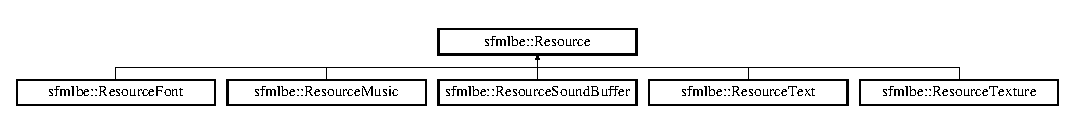
\includegraphics[height=1.197861cm]{classsfmlbe_1_1_resource}
\end{center}
\end{figure}
\subsection*{Public Member Functions}
\begin{DoxyCompactItemize}
\item 
\mbox{\hyperlink{classsfmlbe_1_1_resource_afc4c45a3b69da3904ab98d8096a5dbf6}{Resource}} ()
\begin{DoxyCompactList}\small\item\em Constructor. \end{DoxyCompactList}\item 
\mbox{\hyperlink{classsfmlbe_1_1_resource_a93030eb6f15353680a352fe10b204842}{Resource}} (std\+::string ID, std\+::string filename)
\begin{DoxyCompactList}\small\item\em Constructor. \end{DoxyCompactList}\item 
virtual \mbox{\hyperlink{classsfmlbe_1_1_resource_a54ad6b8a18e74283c707ec1622c94f9f}{$\sim$\+Resource}} ()
\begin{DoxyCompactList}\small\item\em Virtual descructor. \end{DoxyCompactList}\item 
virtual void \mbox{\hyperlink{classsfmlbe_1_1_resource_a35981869a1e90ebbf30258ff7aa1d6d2}{Load}} ()=0
\begin{DoxyCompactList}\small\item\em Virtual member. Used to load the resource. \end{DoxyCompactList}\item 
virtual void \mbox{\hyperlink{classsfmlbe_1_1_resource_a48c75a88679cf457965dd013f47014b9}{Unload}} ()=0
\begin{DoxyCompactList}\small\item\em Virtual member. Used to unload the resource. \end{DoxyCompactList}\item 
void \mbox{\hyperlink{classsfmlbe_1_1_resource_a5f3c845ac15aa355434fe79baca5a019}{Set\+Resource\+ID}} (std\+::string ID)
\begin{DoxyCompactList}\small\item\em Set the resource ID. \end{DoxyCompactList}\item 
std\+::string \mbox{\hyperlink{classsfmlbe_1_1_resource_ae1fb20f1b0e913db9714be96612556c0}{Get\+Resource\+ID}} () const
\begin{DoxyCompactList}\small\item\em Get the resource ID. \end{DoxyCompactList}\item 
void \mbox{\hyperlink{classsfmlbe_1_1_resource_a219b033dc969ca0860bf7402da27107d}{Set\+Filename}} (std\+::string filename)
\begin{DoxyCompactList}\small\item\em Set the resource filename. \end{DoxyCompactList}\item 
std\+::string \mbox{\hyperlink{classsfmlbe_1_1_resource_ae76151a96999e65307a625d1b57cdc80}{Get\+Filename}} () const
\begin{DoxyCompactList}\small\item\em Get the resource filename. \end{DoxyCompactList}\item 
void \mbox{\hyperlink{classsfmlbe_1_1_resource_a6d4c41250bf66f2fe81d4a53d867c4ed}{Set\+Resource\+Type}} (\mbox{\hyperlink{namespacesfmlbe_ac4335ed3060bba025f73e01f9dccb2dd}{R\+E\+S\+O\+U\+R\+C\+E\+\_\+\+T\+Y\+PE}} type)
\begin{DoxyCompactList}\small\item\em Set the resource type. \end{DoxyCompactList}\item 
\mbox{\hyperlink{namespacesfmlbe_ac4335ed3060bba025f73e01f9dccb2dd}{R\+E\+S\+O\+U\+R\+C\+E\+\_\+\+T\+Y\+PE}} \mbox{\hyperlink{classsfmlbe_1_1_resource_a8e0ab17344e90a3c1175a8aa87a96c35}{Get\+Resource\+Type}} () const
\begin{DoxyCompactList}\small\item\em Get the resource type. \end{DoxyCompactList}\item 
bool \mbox{\hyperlink{classsfmlbe_1_1_resource_acd0812c81f7d5d851a4671f0cf7bb4f1}{Is\+Loaded}} () const
\begin{DoxyCompactList}\small\item\em Get if the resource is loaded. \end{DoxyCompactList}\end{DoxyCompactItemize}
\subsection*{Protected Attributes}
\begin{DoxyCompactItemize}
\item 
\mbox{\Hypertarget{classsfmlbe_1_1_resource_a9b6ee23d56d056a440005ac7fb0445ab}\label{classsfmlbe_1_1_resource_a9b6ee23d56d056a440005ac7fb0445ab}} 
std\+::string {\bfseries m\+\_\+resource\+ID}
\item 
\mbox{\Hypertarget{classsfmlbe_1_1_resource_a6819f8b382e2e471a4209731c5b79064}\label{classsfmlbe_1_1_resource_a6819f8b382e2e471a4209731c5b79064}} 
std\+::string {\bfseries m\+\_\+filename}
\item 
\mbox{\Hypertarget{classsfmlbe_1_1_resource_a5f995a7e9f6813a2cb3a1d2f01145410}\label{classsfmlbe_1_1_resource_a5f995a7e9f6813a2cb3a1d2f01145410}} 
\mbox{\hyperlink{namespacesfmlbe_ac4335ed3060bba025f73e01f9dccb2dd}{R\+E\+S\+O\+U\+R\+C\+E\+\_\+\+T\+Y\+PE}} {\bfseries m\+\_\+type}
\item 
\mbox{\Hypertarget{classsfmlbe_1_1_resource_a666c78b37688c4c1a389850f193e97ea}\label{classsfmlbe_1_1_resource_a666c78b37688c4c1a389850f193e97ea}} 
bool {\bfseries m\+\_\+loaded}
\end{DoxyCompactItemize}


\subsection{Detailed Description}
Virtual class representing a \mbox{\hyperlink{classsfmlbe_1_1_resource}{Resource}}. Can be any type of resource listed in R\+E\+S\+O\+U\+R\+C\+E\+\_\+\+T\+Y\+PE, but every type need to be implemented in a child clas, and the \mbox{\hyperlink{classsfmlbe_1_1_resource}{Resource}} Manager need to be updated. 

\subsection{Constructor \& Destructor Documentation}
\mbox{\Hypertarget{classsfmlbe_1_1_resource_afc4c45a3b69da3904ab98d8096a5dbf6}\label{classsfmlbe_1_1_resource_afc4c45a3b69da3904ab98d8096a5dbf6}} 
\index{sfmlbe\+::\+Resource@{sfmlbe\+::\+Resource}!Resource@{Resource}}
\index{Resource@{Resource}!sfmlbe\+::\+Resource@{sfmlbe\+::\+Resource}}
\subsubsection{\texorpdfstring{Resource()}{Resource()}\hspace{0.1cm}{\footnotesize\ttfamily [1/2]}}
{\footnotesize\ttfamily sfmlbe\+::\+Resource\+::\+Resource (\begin{DoxyParamCaption}{ }\end{DoxyParamCaption})\hspace{0.3cm}{\ttfamily [inline]}}



Constructor. 

Construct a non loaded null resource. \begin{DoxySeeAlso}{See also}
\mbox{\hyperlink{classsfmlbe_1_1_resource_a93030eb6f15353680a352fe10b204842}{Resource(std\+::string I\+D, std\+::string filename)}} and \mbox{\hyperlink{classsfmlbe_1_1_resource_a54ad6b8a18e74283c707ec1622c94f9f}{$\sim$\+Resource()}} 
\end{DoxySeeAlso}
\mbox{\Hypertarget{classsfmlbe_1_1_resource_a93030eb6f15353680a352fe10b204842}\label{classsfmlbe_1_1_resource_a93030eb6f15353680a352fe10b204842}} 
\index{sfmlbe\+::\+Resource@{sfmlbe\+::\+Resource}!Resource@{Resource}}
\index{Resource@{Resource}!sfmlbe\+::\+Resource@{sfmlbe\+::\+Resource}}
\subsubsection{\texorpdfstring{Resource()}{Resource()}\hspace{0.1cm}{\footnotesize\ttfamily [2/2]}}
{\footnotesize\ttfamily sfmlbe\+::\+Resource\+::\+Resource (\begin{DoxyParamCaption}\item[{std\+::string}]{ID,  }\item[{std\+::string}]{filename }\end{DoxyParamCaption})\hspace{0.3cm}{\ttfamily [inline]}}



Constructor. 

Construct a non loaded null resource, but with provided parameters. 
\begin{DoxyParams}{Parameters}
{\em ID} & ID of the resource in the scope specified. \\
\hline
{\em filename} & Relative path of file from where the resource is loaded. \\
\hline
\end{DoxyParams}
\begin{DoxySeeAlso}{See also}
\mbox{\hyperlink{classsfmlbe_1_1_resource_afc4c45a3b69da3904ab98d8096a5dbf6}{Resource()}} and \mbox{\hyperlink{classsfmlbe_1_1_resource_a54ad6b8a18e74283c707ec1622c94f9f}{$\sim$\+Resource()}} 
\end{DoxySeeAlso}
\mbox{\Hypertarget{classsfmlbe_1_1_resource_a54ad6b8a18e74283c707ec1622c94f9f}\label{classsfmlbe_1_1_resource_a54ad6b8a18e74283c707ec1622c94f9f}} 
\index{sfmlbe\+::\+Resource@{sfmlbe\+::\+Resource}!````~Resource@{$\sim$\+Resource}}
\index{````~Resource@{$\sim$\+Resource}!sfmlbe\+::\+Resource@{sfmlbe\+::\+Resource}}
\subsubsection{\texorpdfstring{$\sim$\+Resource()}{~Resource()}}
{\footnotesize\ttfamily virtual sfmlbe\+::\+Resource\+::$\sim$\+Resource (\begin{DoxyParamCaption}{ }\end{DoxyParamCaption})\hspace{0.3cm}{\ttfamily [inline]}, {\ttfamily [virtual]}}



Virtual descructor. 

\begin{DoxySeeAlso}{See also}
\mbox{\hyperlink{classsfmlbe_1_1_resource_afc4c45a3b69da3904ab98d8096a5dbf6}{Resource()}} and \mbox{\hyperlink{classsfmlbe_1_1_resource_a93030eb6f15353680a352fe10b204842}{Resource(std\+::string I\+D, std\+::string filename)}} 
\end{DoxySeeAlso}


\subsection{Member Function Documentation}
\mbox{\Hypertarget{classsfmlbe_1_1_resource_ae76151a96999e65307a625d1b57cdc80}\label{classsfmlbe_1_1_resource_ae76151a96999e65307a625d1b57cdc80}} 
\index{sfmlbe\+::\+Resource@{sfmlbe\+::\+Resource}!Get\+Filename@{Get\+Filename}}
\index{Get\+Filename@{Get\+Filename}!sfmlbe\+::\+Resource@{sfmlbe\+::\+Resource}}
\subsubsection{\texorpdfstring{Get\+Filename()}{GetFilename()}}
{\footnotesize\ttfamily std\+::string sfmlbe\+::\+Resource\+::\+Get\+Filename (\begin{DoxyParamCaption}{ }\end{DoxyParamCaption}) const\hspace{0.3cm}{\ttfamily [inline]}}



Get the resource filename. 

\begin{DoxyReturn}{Returns}
Filename of the resource. 
\end{DoxyReturn}
\mbox{\Hypertarget{classsfmlbe_1_1_resource_ae1fb20f1b0e913db9714be96612556c0}\label{classsfmlbe_1_1_resource_ae1fb20f1b0e913db9714be96612556c0}} 
\index{sfmlbe\+::\+Resource@{sfmlbe\+::\+Resource}!Get\+Resource\+ID@{Get\+Resource\+ID}}
\index{Get\+Resource\+ID@{Get\+Resource\+ID}!sfmlbe\+::\+Resource@{sfmlbe\+::\+Resource}}
\subsubsection{\texorpdfstring{Get\+Resource\+I\+D()}{GetResourceID()}}
{\footnotesize\ttfamily std\+::string sfmlbe\+::\+Resource\+::\+Get\+Resource\+ID (\begin{DoxyParamCaption}{ }\end{DoxyParamCaption}) const\hspace{0.3cm}{\ttfamily [inline]}}



Get the resource ID. 

\begin{DoxyReturn}{Returns}
ID of the resource. 
\end{DoxyReturn}
\mbox{\Hypertarget{classsfmlbe_1_1_resource_a8e0ab17344e90a3c1175a8aa87a96c35}\label{classsfmlbe_1_1_resource_a8e0ab17344e90a3c1175a8aa87a96c35}} 
\index{sfmlbe\+::\+Resource@{sfmlbe\+::\+Resource}!Get\+Resource\+Type@{Get\+Resource\+Type}}
\index{Get\+Resource\+Type@{Get\+Resource\+Type}!sfmlbe\+::\+Resource@{sfmlbe\+::\+Resource}}
\subsubsection{\texorpdfstring{Get\+Resource\+Type()}{GetResourceType()}}
{\footnotesize\ttfamily \mbox{\hyperlink{namespacesfmlbe_ac4335ed3060bba025f73e01f9dccb2dd}{R\+E\+S\+O\+U\+R\+C\+E\+\_\+\+T\+Y\+PE}} sfmlbe\+::\+Resource\+::\+Get\+Resource\+Type (\begin{DoxyParamCaption}{ }\end{DoxyParamCaption}) const\hspace{0.3cm}{\ttfamily [inline]}}



Get the resource type. 

\begin{DoxyReturn}{Returns}
\mbox{\hyperlink{classsfmlbe_1_1_resource}{Resource}} type of the resource. 
\end{DoxyReturn}
\mbox{\Hypertarget{classsfmlbe_1_1_resource_acd0812c81f7d5d851a4671f0cf7bb4f1}\label{classsfmlbe_1_1_resource_acd0812c81f7d5d851a4671f0cf7bb4f1}} 
\index{sfmlbe\+::\+Resource@{sfmlbe\+::\+Resource}!Is\+Loaded@{Is\+Loaded}}
\index{Is\+Loaded@{Is\+Loaded}!sfmlbe\+::\+Resource@{sfmlbe\+::\+Resource}}
\subsubsection{\texorpdfstring{Is\+Loaded()}{IsLoaded()}}
{\footnotesize\ttfamily bool sfmlbe\+::\+Resource\+::\+Is\+Loaded (\begin{DoxyParamCaption}{ }\end{DoxyParamCaption}) const\hspace{0.3cm}{\ttfamily [inline]}}



Get if the resource is loaded. 

\begin{DoxyReturn}{Returns}
Is the resource is loaded. 
\end{DoxyReturn}
\mbox{\Hypertarget{classsfmlbe_1_1_resource_a35981869a1e90ebbf30258ff7aa1d6d2}\label{classsfmlbe_1_1_resource_a35981869a1e90ebbf30258ff7aa1d6d2}} 
\index{sfmlbe\+::\+Resource@{sfmlbe\+::\+Resource}!Load@{Load}}
\index{Load@{Load}!sfmlbe\+::\+Resource@{sfmlbe\+::\+Resource}}
\subsubsection{\texorpdfstring{Load()}{Load()}}
{\footnotesize\ttfamily virtual void sfmlbe\+::\+Resource\+::\+Load (\begin{DoxyParamCaption}{ }\end{DoxyParamCaption})\hspace{0.3cm}{\ttfamily [pure virtual]}}



Virtual member. Used to load the resource. 

\begin{DoxySeeAlso}{See also}
\mbox{\hyperlink{classsfmlbe_1_1_resource_a48c75a88679cf457965dd013f47014b9}{Unload()}} 
\end{DoxySeeAlso}


Implemented in \mbox{\hyperlink{classsfmlbe_1_1_resource_text_a1176965f3e9d26c618688f7899b4b58b}{sfmlbe\+::\+Resource\+Text}}, \mbox{\hyperlink{classsfmlbe_1_1_resource_font_a8629842a4597fa4c22e58a85ae76bc74}{sfmlbe\+::\+Resource\+Font}}, \mbox{\hyperlink{classsfmlbe_1_1_resource_music_a8d612eff1f1f8847c2b96a616456e558}{sfmlbe\+::\+Resource\+Music}}, \mbox{\hyperlink{classsfmlbe_1_1_resource_sound_buffer_a1207531bb0e5355f90cf4a7f67734555}{sfmlbe\+::\+Resource\+Sound\+Buffer}}, and \mbox{\hyperlink{classsfmlbe_1_1_resource_texture_a4f8d27c8e50efce6d66a30edb078e2d3}{sfmlbe\+::\+Resource\+Texture}}.

\mbox{\Hypertarget{classsfmlbe_1_1_resource_a219b033dc969ca0860bf7402da27107d}\label{classsfmlbe_1_1_resource_a219b033dc969ca0860bf7402da27107d}} 
\index{sfmlbe\+::\+Resource@{sfmlbe\+::\+Resource}!Set\+Filename@{Set\+Filename}}
\index{Set\+Filename@{Set\+Filename}!sfmlbe\+::\+Resource@{sfmlbe\+::\+Resource}}
\subsubsection{\texorpdfstring{Set\+Filename()}{SetFilename()}}
{\footnotesize\ttfamily void sfmlbe\+::\+Resource\+::\+Set\+Filename (\begin{DoxyParamCaption}\item[{std\+::string}]{filename }\end{DoxyParamCaption})\hspace{0.3cm}{\ttfamily [inline]}}



Set the resource filename. 

Careful with the use of this function. This function does not unload the \mbox{\hyperlink{classsfmlbe_1_1_resource}{Resource}} but set the resource as not loaded. 
\begin{DoxyParams}{Parameters}
{\em filename} & New filename for the resource. \\
\hline
\end{DoxyParams}
\mbox{\Hypertarget{classsfmlbe_1_1_resource_a5f3c845ac15aa355434fe79baca5a019}\label{classsfmlbe_1_1_resource_a5f3c845ac15aa355434fe79baca5a019}} 
\index{sfmlbe\+::\+Resource@{sfmlbe\+::\+Resource}!Set\+Resource\+ID@{Set\+Resource\+ID}}
\index{Set\+Resource\+ID@{Set\+Resource\+ID}!sfmlbe\+::\+Resource@{sfmlbe\+::\+Resource}}
\subsubsection{\texorpdfstring{Set\+Resource\+I\+D()}{SetResourceID()}}
{\footnotesize\ttfamily void sfmlbe\+::\+Resource\+::\+Set\+Resource\+ID (\begin{DoxyParamCaption}\item[{std\+::string}]{ID }\end{DoxyParamCaption})\hspace{0.3cm}{\ttfamily [inline]}}



Set the resource ID. 

Careful with the use of this function. This function does not unload or test if the resource name is unique in his scope. 
\begin{DoxyParams}{Parameters}
{\em ID} & New ID for the resource. \\
\hline
\end{DoxyParams}
\mbox{\Hypertarget{classsfmlbe_1_1_resource_a6d4c41250bf66f2fe81d4a53d867c4ed}\label{classsfmlbe_1_1_resource_a6d4c41250bf66f2fe81d4a53d867c4ed}} 
\index{sfmlbe\+::\+Resource@{sfmlbe\+::\+Resource}!Set\+Resource\+Type@{Set\+Resource\+Type}}
\index{Set\+Resource\+Type@{Set\+Resource\+Type}!sfmlbe\+::\+Resource@{sfmlbe\+::\+Resource}}
\subsubsection{\texorpdfstring{Set\+Resource\+Type()}{SetResourceType()}}
{\footnotesize\ttfamily void sfmlbe\+::\+Resource\+::\+Set\+Resource\+Type (\begin{DoxyParamCaption}\item[{\mbox{\hyperlink{namespacesfmlbe_ac4335ed3060bba025f73e01f9dccb2dd}{R\+E\+S\+O\+U\+R\+C\+E\+\_\+\+T\+Y\+PE}}}]{type }\end{DoxyParamCaption})\hspace{0.3cm}{\ttfamily [inline]}}



Set the resource type. 

Careful with the use of this function. This function does not change the \mbox{\hyperlink{classsfmlbe_1_1_resource}{Resource}} class, but set as not loaded. 
\begin{DoxyParams}{Parameters}
{\em type} & New type for the resource. \\
\hline
\end{DoxyParams}
\mbox{\Hypertarget{classsfmlbe_1_1_resource_a48c75a88679cf457965dd013f47014b9}\label{classsfmlbe_1_1_resource_a48c75a88679cf457965dd013f47014b9}} 
\index{sfmlbe\+::\+Resource@{sfmlbe\+::\+Resource}!Unload@{Unload}}
\index{Unload@{Unload}!sfmlbe\+::\+Resource@{sfmlbe\+::\+Resource}}
\subsubsection{\texorpdfstring{Unload()}{Unload()}}
{\footnotesize\ttfamily virtual void sfmlbe\+::\+Resource\+::\+Unload (\begin{DoxyParamCaption}{ }\end{DoxyParamCaption})\hspace{0.3cm}{\ttfamily [pure virtual]}}



Virtual member. Used to unload the resource. 

\begin{DoxySeeAlso}{See also}
\mbox{\hyperlink{classsfmlbe_1_1_resource_a35981869a1e90ebbf30258ff7aa1d6d2}{Load()}} 
\end{DoxySeeAlso}


Implemented in \mbox{\hyperlink{classsfmlbe_1_1_resource_text_a7493d044dfcd376b0fd17fd5fbd52ada}{sfmlbe\+::\+Resource\+Text}}, \mbox{\hyperlink{classsfmlbe_1_1_resource_font_a44911079325cd8fcf3f2bce64c58ff86}{sfmlbe\+::\+Resource\+Font}}, \mbox{\hyperlink{classsfmlbe_1_1_resource_music_a5697430030c12a5850f317147feb059f}{sfmlbe\+::\+Resource\+Music}}, \mbox{\hyperlink{classsfmlbe_1_1_resource_sound_buffer_aea7707b97d4451935597671c0e162a7b}{sfmlbe\+::\+Resource\+Sound\+Buffer}}, and \mbox{\hyperlink{classsfmlbe_1_1_resource_texture_ac8b1b5866242e222abf0385144711646}{sfmlbe\+::\+Resource\+Texture}}.



The documentation for this class was generated from the following file\+:\begin{DoxyCompactItemize}
\item 
dev/header/\mbox{\hyperlink{resource_8hpp}{resource.\+hpp}}\end{DoxyCompactItemize}

\hypertarget{classsfmlbe_1_1_resource_font}{}\section{sfmlbe\+:\+:Resource\+Font Class Reference}
\label{classsfmlbe_1_1_resource_font}\index{sfmlbe\+::\+Resource\+Font@{sfmlbe\+::\+Resource\+Font}}


{\ttfamily \#include $<$resourcefont.\+hpp$>$}

Inheritance diagram for sfmlbe\+:\+:Resource\+Font\+:\begin{figure}[H]
\begin{center}
\leavevmode
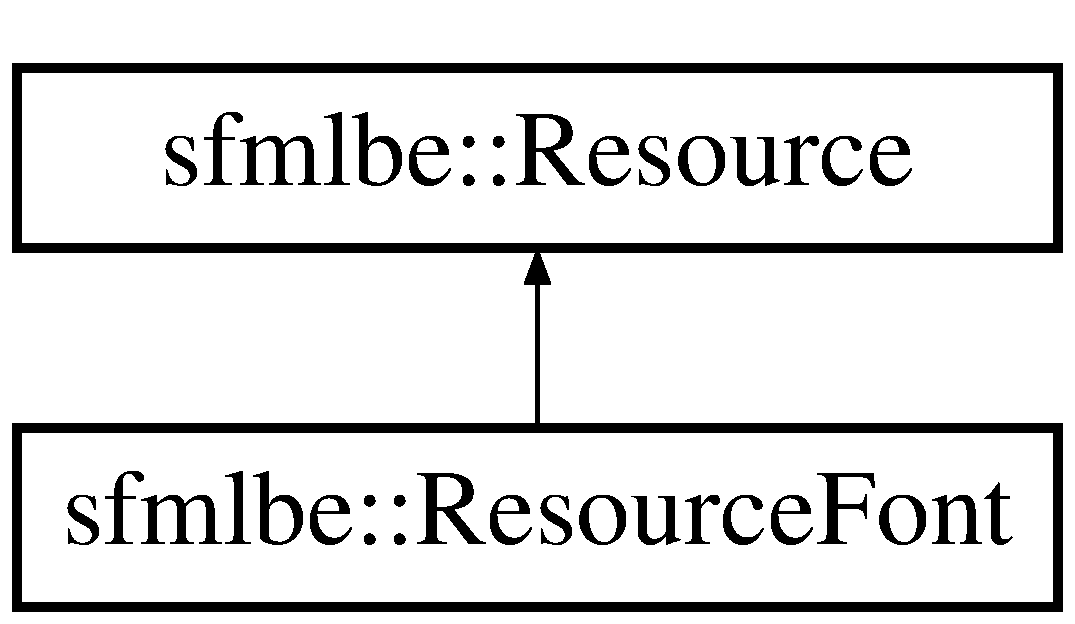
\includegraphics[height=2.000000cm]{classsfmlbe_1_1_resource_font}
\end{center}
\end{figure}
\subsection*{Public Member Functions}
\begin{DoxyCompactItemize}
\item 
\mbox{\hyperlink{classsfmlbe_1_1_resource_font_a1b841c5e14a228a10db8a3d8c6ef2b0b}{Resource\+Font}} ()
\begin{DoxyCompactList}\small\item\em Constructor. \end{DoxyCompactList}\item 
\mbox{\hyperlink{classsfmlbe_1_1_resource_font_ad29b31b52682209630a6a8bba1999200}{Resource\+Font}} (std\+::string ID, std\+::string filename)
\begin{DoxyCompactList}\small\item\em Constructor. \end{DoxyCompactList}\item 
\mbox{\hyperlink{classsfmlbe_1_1_resource_font_a01aa16c3fae9a4027620308008ebbce0}{$\sim$\+Resource\+Font}} ()
\begin{DoxyCompactList}\small\item\em Descructor. \end{DoxyCompactList}\item 
void \mbox{\hyperlink{classsfmlbe_1_1_resource_font_a8629842a4597fa4c22e58a85ae76bc74}{Load}} ()
\begin{DoxyCompactList}\small\item\em Load the sf\+::\+Font targeted by this resource. \end{DoxyCompactList}\item 
void \mbox{\hyperlink{classsfmlbe_1_1_resource_font_a44911079325cd8fcf3f2bce64c58ff86}{Unload}} ()
\begin{DoxyCompactList}\small\item\em Unload the sf\+::\+Font targeted by this resource. \end{DoxyCompactList}\item 
sf\+::\+Font $\ast$ \mbox{\hyperlink{classsfmlbe_1_1_resource_font_a22f252c36d8554aade52e873d3331cce}{Get\+Font}} ()
\begin{DoxyCompactList}\small\item\em Get the sf\+::\+Font associed to this resource. \end{DoxyCompactList}\end{DoxyCompactItemize}
\subsection*{Additional Inherited Members}


\subsection{Detailed Description}
Class allowing to store a sf\+::\+Font using the S\+F\+M\+L\+BE \mbox{\hyperlink{classsfmlbe_1_1_resource}{Resource}} Manager system. Provide an interface to load and unload font easily. 

\subsection{Constructor \& Destructor Documentation}
\mbox{\Hypertarget{classsfmlbe_1_1_resource_font_a1b841c5e14a228a10db8a3d8c6ef2b0b}\label{classsfmlbe_1_1_resource_font_a1b841c5e14a228a10db8a3d8c6ef2b0b}} 
\index{sfmlbe\+::\+Resource\+Font@{sfmlbe\+::\+Resource\+Font}!Resource\+Font@{Resource\+Font}}
\index{Resource\+Font@{Resource\+Font}!sfmlbe\+::\+Resource\+Font@{sfmlbe\+::\+Resource\+Font}}
\subsubsection{\texorpdfstring{Resource\+Font()}{ResourceFont()}\hspace{0.1cm}{\footnotesize\ttfamily [1/2]}}
{\footnotesize\ttfamily sfmlbe\+::\+Resource\+Font\+::\+Resource\+Font (\begin{DoxyParamCaption}{ }\end{DoxyParamCaption})}



Constructor. 

Construct a non loaded font resource. \begin{DoxySeeAlso}{See also}
\mbox{\hyperlink{classsfmlbe_1_1_resource_font_ad29b31b52682209630a6a8bba1999200}{Resource\+Font(std\+::string I\+D, std\+::string filename)}} and \mbox{\hyperlink{classsfmlbe_1_1_resource_font_a01aa16c3fae9a4027620308008ebbce0}{$\sim$\+Resource\+Font()}} 
\end{DoxySeeAlso}
\mbox{\Hypertarget{classsfmlbe_1_1_resource_font_ad29b31b52682209630a6a8bba1999200}\label{classsfmlbe_1_1_resource_font_ad29b31b52682209630a6a8bba1999200}} 
\index{sfmlbe\+::\+Resource\+Font@{sfmlbe\+::\+Resource\+Font}!Resource\+Font@{Resource\+Font}}
\index{Resource\+Font@{Resource\+Font}!sfmlbe\+::\+Resource\+Font@{sfmlbe\+::\+Resource\+Font}}
\subsubsection{\texorpdfstring{Resource\+Font()}{ResourceFont()}\hspace{0.1cm}{\footnotesize\ttfamily [2/2]}}
{\footnotesize\ttfamily sfmlbe\+::\+Resource\+Font\+::\+Resource\+Font (\begin{DoxyParamCaption}\item[{std\+::string}]{ID,  }\item[{std\+::string}]{filename }\end{DoxyParamCaption})}



Constructor. 

Construct a non loaded font resource, but with provided parameters. 
\begin{DoxyParams}{Parameters}
{\em ID} & ID of the resource in the scope specified. \\
\hline
{\em filename} & Relative path of file from where the resource is loaded. \\
\hline
\end{DoxyParams}
\begin{DoxySeeAlso}{See also}
\mbox{\hyperlink{classsfmlbe_1_1_resource_font_a1b841c5e14a228a10db8a3d8c6ef2b0b}{Resource\+Font()}} and \mbox{\hyperlink{classsfmlbe_1_1_resource_font_a01aa16c3fae9a4027620308008ebbce0}{$\sim$\+Resource\+Font()}} 
\end{DoxySeeAlso}
\mbox{\Hypertarget{classsfmlbe_1_1_resource_font_a01aa16c3fae9a4027620308008ebbce0}\label{classsfmlbe_1_1_resource_font_a01aa16c3fae9a4027620308008ebbce0}} 
\index{sfmlbe\+::\+Resource\+Font@{sfmlbe\+::\+Resource\+Font}!````~Resource\+Font@{$\sim$\+Resource\+Font}}
\index{````~Resource\+Font@{$\sim$\+Resource\+Font}!sfmlbe\+::\+Resource\+Font@{sfmlbe\+::\+Resource\+Font}}
\subsubsection{\texorpdfstring{$\sim$\+Resource\+Font()}{~ResourceFont()}}
{\footnotesize\ttfamily sfmlbe\+::\+Resource\+Font\+::$\sim$\+Resource\+Font (\begin{DoxyParamCaption}{ }\end{DoxyParamCaption})}



Descructor. 

Free memory used by the sf\+::\+Font and this resource. \begin{DoxySeeAlso}{See also}
\mbox{\hyperlink{classsfmlbe_1_1_resource_font_a1b841c5e14a228a10db8a3d8c6ef2b0b}{Resource\+Font()}} and \mbox{\hyperlink{classsfmlbe_1_1_resource_font_ad29b31b52682209630a6a8bba1999200}{Resource\+Font(std\+::string I\+D, std\+::string filename)}} 
\end{DoxySeeAlso}


\subsection{Member Function Documentation}
\mbox{\Hypertarget{classsfmlbe_1_1_resource_font_a22f252c36d8554aade52e873d3331cce}\label{classsfmlbe_1_1_resource_font_a22f252c36d8554aade52e873d3331cce}} 
\index{sfmlbe\+::\+Resource\+Font@{sfmlbe\+::\+Resource\+Font}!Get\+Font@{Get\+Font}}
\index{Get\+Font@{Get\+Font}!sfmlbe\+::\+Resource\+Font@{sfmlbe\+::\+Resource\+Font}}
\subsubsection{\texorpdfstring{Get\+Font()}{GetFont()}}
{\footnotesize\ttfamily sf\+::\+Font$\ast$ sfmlbe\+::\+Resource\+Font\+::\+Get\+Font (\begin{DoxyParamCaption}{ }\end{DoxyParamCaption})\hspace{0.3cm}{\ttfamily [inline]}}



Get the sf\+::\+Font associed to this resource. 

\begin{DoxyReturn}{Returns}
Reference to the sf\+::\+Font or N\+U\+LL. 
\end{DoxyReturn}
\mbox{\Hypertarget{classsfmlbe_1_1_resource_font_a8629842a4597fa4c22e58a85ae76bc74}\label{classsfmlbe_1_1_resource_font_a8629842a4597fa4c22e58a85ae76bc74}} 
\index{sfmlbe\+::\+Resource\+Font@{sfmlbe\+::\+Resource\+Font}!Load@{Load}}
\index{Load@{Load}!sfmlbe\+::\+Resource\+Font@{sfmlbe\+::\+Resource\+Font}}
\subsubsection{\texorpdfstring{Load()}{Load()}}
{\footnotesize\ttfamily void sfmlbe\+::\+Resource\+Font\+::\+Load (\begin{DoxyParamCaption}{ }\end{DoxyParamCaption})\hspace{0.3cm}{\ttfamily [virtual]}}



Load the sf\+::\+Font targeted by this resource. 

If success set this resource as loaded. \begin{DoxySeeAlso}{See also}
\mbox{\hyperlink{classsfmlbe_1_1_resource_font_a44911079325cd8fcf3f2bce64c58ff86}{Unload()}} and \mbox{\hyperlink{classsfmlbe_1_1_resource_acd0812c81f7d5d851a4671f0cf7bb4f1}{Is\+Loaded()}} 
\end{DoxySeeAlso}


Implements \mbox{\hyperlink{classsfmlbe_1_1_resource_a35981869a1e90ebbf30258ff7aa1d6d2}{sfmlbe\+::\+Resource}}.

\mbox{\Hypertarget{classsfmlbe_1_1_resource_font_a44911079325cd8fcf3f2bce64c58ff86}\label{classsfmlbe_1_1_resource_font_a44911079325cd8fcf3f2bce64c58ff86}} 
\index{sfmlbe\+::\+Resource\+Font@{sfmlbe\+::\+Resource\+Font}!Unload@{Unload}}
\index{Unload@{Unload}!sfmlbe\+::\+Resource\+Font@{sfmlbe\+::\+Resource\+Font}}
\subsubsection{\texorpdfstring{Unload()}{Unload()}}
{\footnotesize\ttfamily void sfmlbe\+::\+Resource\+Font\+::\+Unload (\begin{DoxyParamCaption}{ }\end{DoxyParamCaption})\hspace{0.3cm}{\ttfamily [virtual]}}



Unload the sf\+::\+Font targeted by this resource. 

If success set this resource as unloaded. \begin{DoxySeeAlso}{See also}
\mbox{\hyperlink{classsfmlbe_1_1_resource_font_a8629842a4597fa4c22e58a85ae76bc74}{Load()}} and \mbox{\hyperlink{classsfmlbe_1_1_resource_acd0812c81f7d5d851a4671f0cf7bb4f1}{Is\+Loaded()}} 
\end{DoxySeeAlso}


Implements \mbox{\hyperlink{classsfmlbe_1_1_resource_a48c75a88679cf457965dd013f47014b9}{sfmlbe\+::\+Resource}}.



The documentation for this class was generated from the following file\+:\begin{DoxyCompactItemize}
\item 
dev/header/\mbox{\hyperlink{resourcefont_8hpp}{resourcefont.\+hpp}}\end{DoxyCompactItemize}

\hypertarget{classsfmlbe_1_1_resource_manager}{}\section{sfmlbe\+:\+:Resource\+Manager Class Reference}
\label{classsfmlbe_1_1_resource_manager}\index{sfmlbe\+::\+Resource\+Manager@{sfmlbe\+::\+Resource\+Manager}}


{\ttfamily \#include $<$resourcemanager.\+hpp$>$}

Inheritance diagram for sfmlbe\+:\+:Resource\+Manager\+:\begin{figure}[H]
\begin{center}
\leavevmode
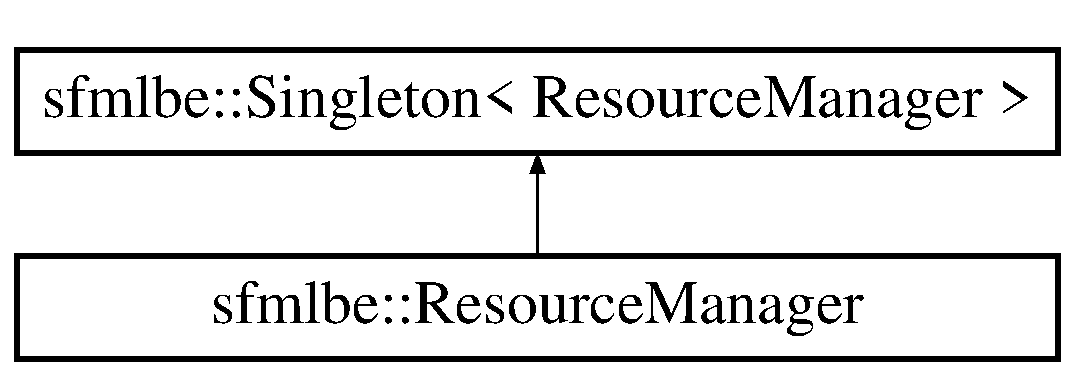
\includegraphics[height=2.000000cm]{classsfmlbe_1_1_resource_manager}
\end{center}
\end{figure}
\subsection*{Public Member Functions}
\begin{DoxyCompactItemize}
\item 
\mbox{\hyperlink{classsfmlbe_1_1_resource}{Resource}} $\ast$ \mbox{\hyperlink{classsfmlbe_1_1_resource_manager_aea559b11d248db65d6bff0caf902098a}{Find\+Resource\+By\+ID}} (const std\+::string \&ID)
\begin{DoxyCompactList}\small\item\em Get a reference on the \mbox{\hyperlink{classsfmlbe_1_1_resource}{Resource}} requested. \end{DoxyCompactList}\item 
\mbox{\hyperlink{classsfmlbe_1_1_resource}{Resource}} $\ast$ \mbox{\hyperlink{classsfmlbe_1_1_resource_manager_a7aa9e19b0a5d525a92ac698ad6497487}{Find\+Resource\+By\+ID}} (const std\+::string \&ID, const std\+::string \&scope)
\begin{DoxyCompactList}\small\item\em Get a reference on the \mbox{\hyperlink{classsfmlbe_1_1_resource}{Resource}} requested. \end{DoxyCompactList}\item 
void \mbox{\hyperlink{classsfmlbe_1_1_resource_manager_a2d25aeeab0779847e3c010ab89c50d0f}{Clear\+Scope}} (const std\+::string \&scopename)
\begin{DoxyCompactList}\small\item\em Clear the scope targeted. \end{DoxyCompactList}\item 
void \mbox{\hyperlink{classsfmlbe_1_1_resource_manager_ae7496b805297eef8c8315ab2437c008c}{Clear}} ()
\begin{DoxyCompactList}\small\item\em Clear all the scopes. \end{DoxyCompactList}\item 
void \mbox{\hyperlink{classsfmlbe_1_1_resource_manager_a8f99da24868d355227f641dc50db2bd2}{Load\+From\+File\+X\+ML}} (const std\+::string \&filename)
\begin{DoxyCompactList}\small\item\em Load \mbox{\hyperlink{classsfmlbe_1_1_resource}{Resource}} indexed in the X\+ML file targeted. \end{DoxyCompactList}\item 
void \mbox{\hyperlink{classsfmlbe_1_1_resource_manager_a2da403b4057837350f5e09f0a33b80dd}{Load\+From\+File\+X\+ML}} (const std\+::string \&filename, const std\+::string \&scopename)
\begin{DoxyCompactList}\small\item\em Load \mbox{\hyperlink{classsfmlbe_1_1_resource}{Resource}} indexed in the X\+ML file targeted with a targeted scope. \end{DoxyCompactList}\item 
void \mbox{\hyperlink{classsfmlbe_1_1_resource_manager_a99707b50bdf61ac1daadd65027a1ae2b}{Load\+From\+File\+X\+ML}} (const std\+::string \&filename, const std\+::string \&scopename, const std\+::string \&scope\+\_\+target)
\begin{DoxyCompactList}\small\item\em Load \mbox{\hyperlink{classsfmlbe_1_1_resource}{Resource}} indexed in the X\+ML file targeted with a targeted scope and add them to another scope. \end{DoxyCompactList}\item 
void \mbox{\hyperlink{classsfmlbe_1_1_resource_manager_a74e64d1b098dcdbc0ee4fd8925303523}{Print\+Manager}} ()
\begin{DoxyCompactList}\small\item\em Print all the resources in the \mbox{\hyperlink{classsfmlbe_1_1_resource}{Resource}} Manager. \end{DoxyCompactList}\item 
U\+I\+NT \mbox{\hyperlink{classsfmlbe_1_1_resource_manager_a99c69873bb1084afe35a97986c657ee9}{Get\+Resource\+Count}} () const
\begin{DoxyCompactList}\small\item\em Get the number of resources loaded. \end{DoxyCompactList}\end{DoxyCompactItemize}
\subsection*{Friends}
\begin{DoxyCompactItemize}
\item 
\mbox{\Hypertarget{classsfmlbe_1_1_resource_manager_a8cc0c523af7e6e454ed0f273b5f18e4a}\label{classsfmlbe_1_1_resource_manager_a8cc0c523af7e6e454ed0f273b5f18e4a}} 
class {\bfseries Singleton$<$ Resource\+Manager $>$}
\end{DoxyCompactItemize}
\subsection*{Additional Inherited Members}


\subsection{Detailed Description}
Class representing a Manager for all the resources. Provide an interface to load and unload resources easily, and to retreive them from anywhere. Use a scope system to provide multiple occurences of a resource and manage multiple contexts easier. 

\subsection{Member Function Documentation}
\mbox{\Hypertarget{classsfmlbe_1_1_resource_manager_ae7496b805297eef8c8315ab2437c008c}\label{classsfmlbe_1_1_resource_manager_ae7496b805297eef8c8315ab2437c008c}} 
\index{sfmlbe\+::\+Resource\+Manager@{sfmlbe\+::\+Resource\+Manager}!Clear@{Clear}}
\index{Clear@{Clear}!sfmlbe\+::\+Resource\+Manager@{sfmlbe\+::\+Resource\+Manager}}
\subsubsection{\texorpdfstring{Clear()}{Clear()}}
{\footnotesize\ttfamily void sfmlbe\+::\+Resource\+Manager\+::\+Clear (\begin{DoxyParamCaption}{ }\end{DoxyParamCaption})}



Clear all the scopes. 

Free memory for all the resources in all scopes, and delete everthing. Reset the \mbox{\hyperlink{classsfmlbe_1_1_resource_manager}{Resource\+Manager}}. \begin{DoxySeeAlso}{See also}
Clear(const std\+::string \& scopename) 
\end{DoxySeeAlso}
\mbox{\Hypertarget{classsfmlbe_1_1_resource_manager_a2d25aeeab0779847e3c010ab89c50d0f}\label{classsfmlbe_1_1_resource_manager_a2d25aeeab0779847e3c010ab89c50d0f}} 
\index{sfmlbe\+::\+Resource\+Manager@{sfmlbe\+::\+Resource\+Manager}!Clear\+Scope@{Clear\+Scope}}
\index{Clear\+Scope@{Clear\+Scope}!sfmlbe\+::\+Resource\+Manager@{sfmlbe\+::\+Resource\+Manager}}
\subsubsection{\texorpdfstring{Clear\+Scope()}{ClearScope()}}
{\footnotesize\ttfamily void sfmlbe\+::\+Resource\+Manager\+::\+Clear\+Scope (\begin{DoxyParamCaption}\item[{const std\+::string \&}]{scopename }\end{DoxyParamCaption})}



Clear the scope targeted. 

Free memory for all the resources in the scope, and delete it. If he does not exist, do nothing. 
\begin{DoxyParams}{Parameters}
{\em scopename} & Name of the scope to clear. \\
\hline
\end{DoxyParams}
\begin{DoxySeeAlso}{See also}
\mbox{\hyperlink{classsfmlbe_1_1_resource_manager_ae7496b805297eef8c8315ab2437c008c}{Clear()}} 
\end{DoxySeeAlso}
\mbox{\Hypertarget{classsfmlbe_1_1_resource_manager_aea559b11d248db65d6bff0caf902098a}\label{classsfmlbe_1_1_resource_manager_aea559b11d248db65d6bff0caf902098a}} 
\index{sfmlbe\+::\+Resource\+Manager@{sfmlbe\+::\+Resource\+Manager}!Find\+Resource\+By\+ID@{Find\+Resource\+By\+ID}}
\index{Find\+Resource\+By\+ID@{Find\+Resource\+By\+ID}!sfmlbe\+::\+Resource\+Manager@{sfmlbe\+::\+Resource\+Manager}}
\subsubsection{\texorpdfstring{Find\+Resource\+By\+I\+D()}{FindResourceByID()}\hspace{0.1cm}{\footnotesize\ttfamily [1/2]}}
{\footnotesize\ttfamily \mbox{\hyperlink{classsfmlbe_1_1_resource}{Resource}}$\ast$ sfmlbe\+::\+Resource\+Manager\+::\+Find\+Resource\+By\+ID (\begin{DoxyParamCaption}\item[{const std\+::string \&}]{ID }\end{DoxyParamCaption})}



Get a reference on the \mbox{\hyperlink{classsfmlbe_1_1_resource}{Resource}} requested. 

Return the first occurrence of the \mbox{\hyperlink{classsfmlbe_1_1_resource}{Resource}} requested in all scopes loaded. \mbox{\hyperlink{classsfmlbe_1_1_resource}{Resource}} could be any type listed in R\+E\+S\+O\+U\+R\+C\+E\+\_\+\+T\+Y\+PE. 
\begin{DoxyExceptions}{Exceptions}
{\em \mbox{\hyperlink{classsfmlbe_1_1_resource_not_found_exception}{sfmlbe\+::\+Resource\+Not\+Found\+Exception}}} & if the resource is not found in any scope. \\
\hline
\end{DoxyExceptions}

\begin{DoxyParams}{Parameters}
{\em ID} & ID of the resource . \\
\hline
\end{DoxyParams}
\begin{DoxyReturn}{Returns}
Reference on the \mbox{\hyperlink{classsfmlbe_1_1_resource}{sfmlbe\+::\+Resource}} or throws exception. 
\end{DoxyReturn}
\begin{DoxySeeAlso}{See also}
\mbox{\hyperlink{classsfmlbe_1_1_resource_manager_a7aa9e19b0a5d525a92ac698ad6497487}{Find\+Resource\+By\+I\+D(const std\+::string \& I\+D, const std\+::string \& scope)}} 
\end{DoxySeeAlso}
\mbox{\Hypertarget{classsfmlbe_1_1_resource_manager_a7aa9e19b0a5d525a92ac698ad6497487}\label{classsfmlbe_1_1_resource_manager_a7aa9e19b0a5d525a92ac698ad6497487}} 
\index{sfmlbe\+::\+Resource\+Manager@{sfmlbe\+::\+Resource\+Manager}!Find\+Resource\+By\+ID@{Find\+Resource\+By\+ID}}
\index{Find\+Resource\+By\+ID@{Find\+Resource\+By\+ID}!sfmlbe\+::\+Resource\+Manager@{sfmlbe\+::\+Resource\+Manager}}
\subsubsection{\texorpdfstring{Find\+Resource\+By\+I\+D()}{FindResourceByID()}\hspace{0.1cm}{\footnotesize\ttfamily [2/2]}}
{\footnotesize\ttfamily \mbox{\hyperlink{classsfmlbe_1_1_resource}{Resource}}$\ast$ sfmlbe\+::\+Resource\+Manager\+::\+Find\+Resource\+By\+ID (\begin{DoxyParamCaption}\item[{const std\+::string \&}]{ID,  }\item[{const std\+::string \&}]{scope }\end{DoxyParamCaption})}



Get a reference on the \mbox{\hyperlink{classsfmlbe_1_1_resource}{Resource}} requested. 

Return the occurence of the \mbox{\hyperlink{classsfmlbe_1_1_resource}{Resource}} requested in the scope targeted. \mbox{\hyperlink{classsfmlbe_1_1_resource}{Resource}} could be any type listed in R\+E\+S\+O\+U\+R\+C\+E\+\_\+\+T\+Y\+PE. 
\begin{DoxyExceptions}{Exceptions}
{\em \mbox{\hyperlink{classsfmlbe_1_1_resource_not_found_exception}{sfmlbe\+::\+Resource\+Not\+Found\+Exception}}} & if the resource is not found in the scope. \\
\hline
{\em \mbox{\hyperlink{classsfmlbe_1_1_scope_not_found_exception}{sfmlbe\+::\+Scope\+Not\+Found\+Exception}}} & if the scope is not found. \\
\hline
\end{DoxyExceptions}

\begin{DoxyParams}{Parameters}
{\em ID} & ID of the resource. \\
\hline
{\em scope} & Name of the scope where to search the resource. \\
\hline
\end{DoxyParams}
\begin{DoxyReturn}{Returns}
Reference on the \mbox{\hyperlink{classsfmlbe_1_1_resource}{sfmlbe\+::\+Resource}} or throws exception. 
\end{DoxyReturn}
\begin{DoxySeeAlso}{See also}
\mbox{\hyperlink{classsfmlbe_1_1_resource_manager_aea559b11d248db65d6bff0caf902098a}{Find\+Resource\+By\+I\+D(const std\+::string \& I\+D)}} 
\end{DoxySeeAlso}
\mbox{\Hypertarget{classsfmlbe_1_1_resource_manager_a99c69873bb1084afe35a97986c657ee9}\label{classsfmlbe_1_1_resource_manager_a99c69873bb1084afe35a97986c657ee9}} 
\index{sfmlbe\+::\+Resource\+Manager@{sfmlbe\+::\+Resource\+Manager}!Get\+Resource\+Count@{Get\+Resource\+Count}}
\index{Get\+Resource\+Count@{Get\+Resource\+Count}!sfmlbe\+::\+Resource\+Manager@{sfmlbe\+::\+Resource\+Manager}}
\subsubsection{\texorpdfstring{Get\+Resource\+Count()}{GetResourceCount()}}
{\footnotesize\ttfamily U\+I\+NT sfmlbe\+::\+Resource\+Manager\+::\+Get\+Resource\+Count (\begin{DoxyParamCaption}{ }\end{DoxyParamCaption}) const\hspace{0.3cm}{\ttfamily [inline]}}



Get the number of resources loaded. 

\begin{DoxyReturn}{Returns}
Number of resources loaded. 
\end{DoxyReturn}
\mbox{\Hypertarget{classsfmlbe_1_1_resource_manager_a8f99da24868d355227f641dc50db2bd2}\label{classsfmlbe_1_1_resource_manager_a8f99da24868d355227f641dc50db2bd2}} 
\index{sfmlbe\+::\+Resource\+Manager@{sfmlbe\+::\+Resource\+Manager}!Load\+From\+File\+X\+ML@{Load\+From\+File\+X\+ML}}
\index{Load\+From\+File\+X\+ML@{Load\+From\+File\+X\+ML}!sfmlbe\+::\+Resource\+Manager@{sfmlbe\+::\+Resource\+Manager}}
\subsubsection{\texorpdfstring{Load\+From\+File\+X\+M\+L()}{LoadFromFileXML()}\hspace{0.1cm}{\footnotesize\ttfamily [1/3]}}
{\footnotesize\ttfamily void sfmlbe\+::\+Resource\+Manager\+::\+Load\+From\+File\+X\+ML (\begin{DoxyParamCaption}\item[{const std\+::string \&}]{filename }\end{DoxyParamCaption})}



Load \mbox{\hyperlink{classsfmlbe_1_1_resource}{Resource}} indexed in the X\+ML file targeted. 

Try to load every resource indexed in the filename in the first valid scope. Creates the scope or appends the resources if the scope already exists. If some identical keys are already in it, they will be replaced ! Filename and resources need to be in the data folder (see examples). 
\begin{DoxyParams}{Parameters}
{\em filename} & Name of the indexer where all the resources are listes. \\
\hline
\end{DoxyParams}
\begin{DoxySeeAlso}{See also}
\mbox{\hyperlink{classsfmlbe_1_1_resource_manager_a2da403b4057837350f5e09f0a33b80dd}{Load\+From\+File\+X\+M\+L(const std\+::string \& filename, const std\+::string \& scopename)}} and \mbox{\hyperlink{classsfmlbe_1_1_resource_manager_a99707b50bdf61ac1daadd65027a1ae2b}{Load\+From\+File\+X\+M\+L(const std\+::string \& filename, const std\+::string \& scopename, const std\+::string \& scope\+\_\+target)}} 
\end{DoxySeeAlso}
\mbox{\Hypertarget{classsfmlbe_1_1_resource_manager_a2da403b4057837350f5e09f0a33b80dd}\label{classsfmlbe_1_1_resource_manager_a2da403b4057837350f5e09f0a33b80dd}} 
\index{sfmlbe\+::\+Resource\+Manager@{sfmlbe\+::\+Resource\+Manager}!Load\+From\+File\+X\+ML@{Load\+From\+File\+X\+ML}}
\index{Load\+From\+File\+X\+ML@{Load\+From\+File\+X\+ML}!sfmlbe\+::\+Resource\+Manager@{sfmlbe\+::\+Resource\+Manager}}
\subsubsection{\texorpdfstring{Load\+From\+File\+X\+M\+L()}{LoadFromFileXML()}\hspace{0.1cm}{\footnotesize\ttfamily [2/3]}}
{\footnotesize\ttfamily void sfmlbe\+::\+Resource\+Manager\+::\+Load\+From\+File\+X\+ML (\begin{DoxyParamCaption}\item[{const std\+::string \&}]{filename,  }\item[{const std\+::string \&}]{scopename }\end{DoxyParamCaption})}



Load \mbox{\hyperlink{classsfmlbe_1_1_resource}{Resource}} indexed in the X\+ML file targeted with a targeted scope. 

Try to load every resource indexed in the filename in the targeted scope. Creates the scope or appends the resources if the scope already exists. If some identical keys are already in it, they will be replaced ! Filename and resources need to be in the data folder (see examples). 
\begin{DoxyParams}{Parameters}
{\em filename} & Name of the indexer where all the resources are listes. \\
\hline
{\em scopename} & Name of the scope wanted in filename. \\
\hline
\end{DoxyParams}
\begin{DoxySeeAlso}{See also}
\mbox{\hyperlink{classsfmlbe_1_1_resource_manager_a8f99da24868d355227f641dc50db2bd2}{Load\+From\+File\+X\+M\+L()}} and \mbox{\hyperlink{classsfmlbe_1_1_resource_manager_a99707b50bdf61ac1daadd65027a1ae2b}{Load\+From\+File\+X\+M\+L(const std\+::string \& filename, const std\+::string \& scopename, const std\+::string \& scope\+\_\+target)}} 
\end{DoxySeeAlso}
\mbox{\Hypertarget{classsfmlbe_1_1_resource_manager_a99707b50bdf61ac1daadd65027a1ae2b}\label{classsfmlbe_1_1_resource_manager_a99707b50bdf61ac1daadd65027a1ae2b}} 
\index{sfmlbe\+::\+Resource\+Manager@{sfmlbe\+::\+Resource\+Manager}!Load\+From\+File\+X\+ML@{Load\+From\+File\+X\+ML}}
\index{Load\+From\+File\+X\+ML@{Load\+From\+File\+X\+ML}!sfmlbe\+::\+Resource\+Manager@{sfmlbe\+::\+Resource\+Manager}}
\subsubsection{\texorpdfstring{Load\+From\+File\+X\+M\+L()}{LoadFromFileXML()}\hspace{0.1cm}{\footnotesize\ttfamily [3/3]}}
{\footnotesize\ttfamily void sfmlbe\+::\+Resource\+Manager\+::\+Load\+From\+File\+X\+ML (\begin{DoxyParamCaption}\item[{const std\+::string \&}]{filename,  }\item[{const std\+::string \&}]{scopename,  }\item[{const std\+::string \&}]{scope\+\_\+target }\end{DoxyParamCaption})}



Load \mbox{\hyperlink{classsfmlbe_1_1_resource}{Resource}} indexed in the X\+ML file targeted with a targeted scope and add them to another scope. 

Try to load every resource indexed in the filename in the targeted scope and append them to anoter scope. Creates the scope targeted or appends the resources if the scope already exists. If some identical keys are already in it, they will be replaced ! Filename and resources need to be in the data folder (see examples). 
\begin{DoxyParams}{Parameters}
{\em filename} & Name of the indexer where all the resources are listes. \\
\hline
{\em scopename} & Name of the scope wanted in filename. \\
\hline
{\em scope\+\_\+target} & Name of the scope where append resources. \\
\hline
\end{DoxyParams}
\begin{DoxySeeAlso}{See also}
\mbox{\hyperlink{classsfmlbe_1_1_resource_manager_a8f99da24868d355227f641dc50db2bd2}{Load\+From\+File\+X\+M\+L()}} and \mbox{\hyperlink{classsfmlbe_1_1_resource_manager_a2da403b4057837350f5e09f0a33b80dd}{Load\+From\+File\+X\+M\+L(const std\+::string \& filename, const std\+::string \& scopename)}} 
\end{DoxySeeAlso}
\mbox{\Hypertarget{classsfmlbe_1_1_resource_manager_a74e64d1b098dcdbc0ee4fd8925303523}\label{classsfmlbe_1_1_resource_manager_a74e64d1b098dcdbc0ee4fd8925303523}} 
\index{sfmlbe\+::\+Resource\+Manager@{sfmlbe\+::\+Resource\+Manager}!Print\+Manager@{Print\+Manager}}
\index{Print\+Manager@{Print\+Manager}!sfmlbe\+::\+Resource\+Manager@{sfmlbe\+::\+Resource\+Manager}}
\subsubsection{\texorpdfstring{Print\+Manager()}{PrintManager()}}
{\footnotesize\ttfamily void sfmlbe\+::\+Resource\+Manager\+::\+Print\+Manager (\begin{DoxyParamCaption}{ }\end{DoxyParamCaption})}



Print all the resources in the \mbox{\hyperlink{classsfmlbe_1_1_resource}{Resource}} Manager. 

Do what it says. 

The documentation for this class was generated from the following file\+:\begin{DoxyCompactItemize}
\item 
dev/header/\mbox{\hyperlink{resourcemanager_8hpp}{resourcemanager.\+hpp}}\end{DoxyCompactItemize}

\hypertarget{classsfmlbe_1_1_resource_music}{}\section{sfmlbe\+:\+:Resource\+Music Class Reference}
\label{classsfmlbe_1_1_resource_music}\index{sfmlbe\+::\+Resource\+Music@{sfmlbe\+::\+Resource\+Music}}


{\ttfamily \#include $<$resourcemusic.\+hpp$>$}

Inheritance diagram for sfmlbe\+:\+:Resource\+Music\+:\begin{figure}[H]
\begin{center}
\leavevmode
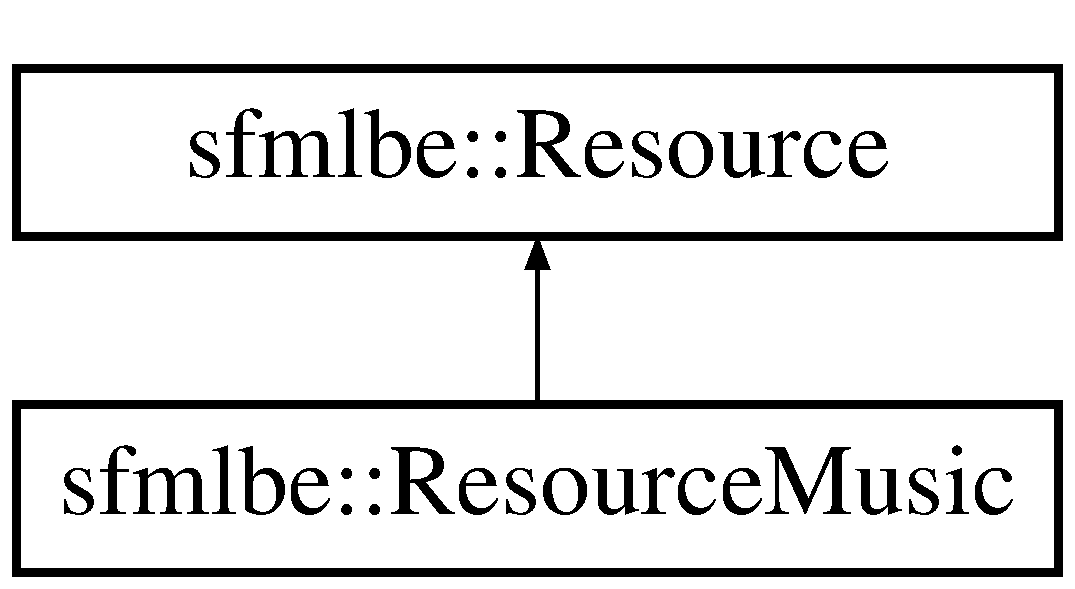
\includegraphics[height=2.000000cm]{classsfmlbe_1_1_resource_music}
\end{center}
\end{figure}
\subsection*{Public Member Functions}
\begin{DoxyCompactItemize}
\item 
\mbox{\hyperlink{classsfmlbe_1_1_resource_music_a9a20ebb5669632cbc4d85afb6ecf8848}{Resource\+Music}} ()
\begin{DoxyCompactList}\small\item\em Constructor. \end{DoxyCompactList}\item 
\mbox{\hyperlink{classsfmlbe_1_1_resource_music_a31e4aa77dd956096604e3b939e3d2075}{Resource\+Music}} (std\+::string ID, std\+::string filename)
\begin{DoxyCompactList}\small\item\em Constructor. \end{DoxyCompactList}\item 
\mbox{\hyperlink{classsfmlbe_1_1_resource_music_a13f5a79c13b15951d855cad9224a1a7b}{$\sim$\+Resource\+Music}} ()
\begin{DoxyCompactList}\small\item\em Descructor. \end{DoxyCompactList}\item 
void \mbox{\hyperlink{classsfmlbe_1_1_resource_music_a8d612eff1f1f8847c2b96a616456e558}{Load}} ()
\begin{DoxyCompactList}\small\item\em Load the sf\+::\+Music targeted by this resource. \end{DoxyCompactList}\item 
void \mbox{\hyperlink{classsfmlbe_1_1_resource_music_a5697430030c12a5850f317147feb059f}{Unload}} ()
\begin{DoxyCompactList}\small\item\em Unload the sf\+::\+Music targeted by this resource. \end{DoxyCompactList}\item 
sf\+::\+Music $\ast$ \mbox{\hyperlink{classsfmlbe_1_1_resource_music_a2092277768f71da98fac91d2d37c898c}{Get\+Music}} ()
\begin{DoxyCompactList}\small\item\em Get the sf\+::\+Music associed to this resource. \end{DoxyCompactList}\end{DoxyCompactItemize}
\subsection*{Additional Inherited Members}


\subsection{Detailed Description}
Class allowing to store a sf\+::\+Music using the S\+F\+M\+L\+BE \mbox{\hyperlink{classsfmlbe_1_1_resource}{Resource}} Manager system. Provide an interface to load and unload music easily. 

\subsection{Constructor \& Destructor Documentation}
\mbox{\Hypertarget{classsfmlbe_1_1_resource_music_a9a20ebb5669632cbc4d85afb6ecf8848}\label{classsfmlbe_1_1_resource_music_a9a20ebb5669632cbc4d85afb6ecf8848}} 
\index{sfmlbe\+::\+Resource\+Music@{sfmlbe\+::\+Resource\+Music}!Resource\+Music@{Resource\+Music}}
\index{Resource\+Music@{Resource\+Music}!sfmlbe\+::\+Resource\+Music@{sfmlbe\+::\+Resource\+Music}}
\subsubsection{\texorpdfstring{Resource\+Music()}{ResourceMusic()}\hspace{0.1cm}{\footnotesize\ttfamily [1/2]}}
{\footnotesize\ttfamily sfmlbe\+::\+Resource\+Music\+::\+Resource\+Music (\begin{DoxyParamCaption}{ }\end{DoxyParamCaption})}



Constructor. 

Construct a non loaded music resource. \begin{DoxySeeAlso}{See also}
\mbox{\hyperlink{classsfmlbe_1_1_resource_music_a31e4aa77dd956096604e3b939e3d2075}{Resource\+Music(std\+::string I\+D, std\+::string filename)}} and \mbox{\hyperlink{classsfmlbe_1_1_resource_music_a13f5a79c13b15951d855cad9224a1a7b}{$\sim$\+Resource\+Music()}} 
\end{DoxySeeAlso}
\mbox{\Hypertarget{classsfmlbe_1_1_resource_music_a31e4aa77dd956096604e3b939e3d2075}\label{classsfmlbe_1_1_resource_music_a31e4aa77dd956096604e3b939e3d2075}} 
\index{sfmlbe\+::\+Resource\+Music@{sfmlbe\+::\+Resource\+Music}!Resource\+Music@{Resource\+Music}}
\index{Resource\+Music@{Resource\+Music}!sfmlbe\+::\+Resource\+Music@{sfmlbe\+::\+Resource\+Music}}
\subsubsection{\texorpdfstring{Resource\+Music()}{ResourceMusic()}\hspace{0.1cm}{\footnotesize\ttfamily [2/2]}}
{\footnotesize\ttfamily sfmlbe\+::\+Resource\+Music\+::\+Resource\+Music (\begin{DoxyParamCaption}\item[{std\+::string}]{ID,  }\item[{std\+::string}]{filename }\end{DoxyParamCaption})}



Constructor. 

Construct a non loaded music resource, but with provided parameters. 
\begin{DoxyParams}{Parameters}
{\em ID} & ID of the resource in the scope specified. \\
\hline
{\em filename} & Relative path of file from where the resource is loaded. \\
\hline
\end{DoxyParams}
\begin{DoxySeeAlso}{See also}
\mbox{\hyperlink{classsfmlbe_1_1_resource_music_a9a20ebb5669632cbc4d85afb6ecf8848}{Resource\+Music()}} and \mbox{\hyperlink{classsfmlbe_1_1_resource_music_a13f5a79c13b15951d855cad9224a1a7b}{$\sim$\+Resource\+Music()}} 
\end{DoxySeeAlso}
\mbox{\Hypertarget{classsfmlbe_1_1_resource_music_a13f5a79c13b15951d855cad9224a1a7b}\label{classsfmlbe_1_1_resource_music_a13f5a79c13b15951d855cad9224a1a7b}} 
\index{sfmlbe\+::\+Resource\+Music@{sfmlbe\+::\+Resource\+Music}!````~Resource\+Music@{$\sim$\+Resource\+Music}}
\index{````~Resource\+Music@{$\sim$\+Resource\+Music}!sfmlbe\+::\+Resource\+Music@{sfmlbe\+::\+Resource\+Music}}
\subsubsection{\texorpdfstring{$\sim$\+Resource\+Music()}{~ResourceMusic()}}
{\footnotesize\ttfamily sfmlbe\+::\+Resource\+Music\+::$\sim$\+Resource\+Music (\begin{DoxyParamCaption}{ }\end{DoxyParamCaption})}



Descructor. 

Free memory used by the sf\+::\+Music and this resource. \begin{DoxySeeAlso}{See also}
\mbox{\hyperlink{classsfmlbe_1_1_resource_music_a9a20ebb5669632cbc4d85afb6ecf8848}{Resource\+Music()}} and \mbox{\hyperlink{classsfmlbe_1_1_resource_music_a31e4aa77dd956096604e3b939e3d2075}{Resource\+Music(std\+::string I\+D, std\+::string filename)}} 
\end{DoxySeeAlso}


\subsection{Member Function Documentation}
\mbox{\Hypertarget{classsfmlbe_1_1_resource_music_a2092277768f71da98fac91d2d37c898c}\label{classsfmlbe_1_1_resource_music_a2092277768f71da98fac91d2d37c898c}} 
\index{sfmlbe\+::\+Resource\+Music@{sfmlbe\+::\+Resource\+Music}!Get\+Music@{Get\+Music}}
\index{Get\+Music@{Get\+Music}!sfmlbe\+::\+Resource\+Music@{sfmlbe\+::\+Resource\+Music}}
\subsubsection{\texorpdfstring{Get\+Music()}{GetMusic()}}
{\footnotesize\ttfamily sf\+::\+Music$\ast$ sfmlbe\+::\+Resource\+Music\+::\+Get\+Music (\begin{DoxyParamCaption}{ }\end{DoxyParamCaption})\hspace{0.3cm}{\ttfamily [inline]}}



Get the sf\+::\+Music associed to this resource. 

\begin{DoxyReturn}{Returns}
Reference to the sf\+::\+Music or N\+U\+LL. 
\end{DoxyReturn}
\mbox{\Hypertarget{classsfmlbe_1_1_resource_music_a8d612eff1f1f8847c2b96a616456e558}\label{classsfmlbe_1_1_resource_music_a8d612eff1f1f8847c2b96a616456e558}} 
\index{sfmlbe\+::\+Resource\+Music@{sfmlbe\+::\+Resource\+Music}!Load@{Load}}
\index{Load@{Load}!sfmlbe\+::\+Resource\+Music@{sfmlbe\+::\+Resource\+Music}}
\subsubsection{\texorpdfstring{Load()}{Load()}}
{\footnotesize\ttfamily void sfmlbe\+::\+Resource\+Music\+::\+Load (\begin{DoxyParamCaption}{ }\end{DoxyParamCaption})\hspace{0.3cm}{\ttfamily [virtual]}}



Load the sf\+::\+Music targeted by this resource. 

If success set this resource as loaded. \begin{DoxySeeAlso}{See also}
\mbox{\hyperlink{classsfmlbe_1_1_resource_music_a5697430030c12a5850f317147feb059f}{Unload()}} and \mbox{\hyperlink{classsfmlbe_1_1_resource_acd0812c81f7d5d851a4671f0cf7bb4f1}{Is\+Loaded()}} 
\end{DoxySeeAlso}


Implements \mbox{\hyperlink{classsfmlbe_1_1_resource_a35981869a1e90ebbf30258ff7aa1d6d2}{sfmlbe\+::\+Resource}}.

\mbox{\Hypertarget{classsfmlbe_1_1_resource_music_a5697430030c12a5850f317147feb059f}\label{classsfmlbe_1_1_resource_music_a5697430030c12a5850f317147feb059f}} 
\index{sfmlbe\+::\+Resource\+Music@{sfmlbe\+::\+Resource\+Music}!Unload@{Unload}}
\index{Unload@{Unload}!sfmlbe\+::\+Resource\+Music@{sfmlbe\+::\+Resource\+Music}}
\subsubsection{\texorpdfstring{Unload()}{Unload()}}
{\footnotesize\ttfamily void sfmlbe\+::\+Resource\+Music\+::\+Unload (\begin{DoxyParamCaption}{ }\end{DoxyParamCaption})\hspace{0.3cm}{\ttfamily [virtual]}}



Unload the sf\+::\+Music targeted by this resource. 

If success set this resource as unloaded. \begin{DoxySeeAlso}{See also}
\mbox{\hyperlink{classsfmlbe_1_1_resource_music_a8d612eff1f1f8847c2b96a616456e558}{Load()}} and \mbox{\hyperlink{classsfmlbe_1_1_resource_acd0812c81f7d5d851a4671f0cf7bb4f1}{Is\+Loaded()}} 
\end{DoxySeeAlso}


Implements \mbox{\hyperlink{classsfmlbe_1_1_resource_a48c75a88679cf457965dd013f47014b9}{sfmlbe\+::\+Resource}}.



The documentation for this class was generated from the following file\+:\begin{DoxyCompactItemize}
\item 
dev/header/\mbox{\hyperlink{resourcemusic_8hpp}{resourcemusic.\+hpp}}\end{DoxyCompactItemize}

\hypertarget{classsfmlbe_1_1_resource_not_found_exception}{}\section{sfmlbe\+:\+:Resource\+Not\+Found\+Exception Class Reference}
\label{classsfmlbe_1_1_resource_not_found_exception}\index{sfmlbe\+::\+Resource\+Not\+Found\+Exception@{sfmlbe\+::\+Resource\+Not\+Found\+Exception}}


{\ttfamily \#include $<$resourceexceptions.\+hpp$>$}

Inheritance diagram for sfmlbe\+:\+:Resource\+Not\+Found\+Exception\+:\begin{figure}[H]
\begin{center}
\leavevmode
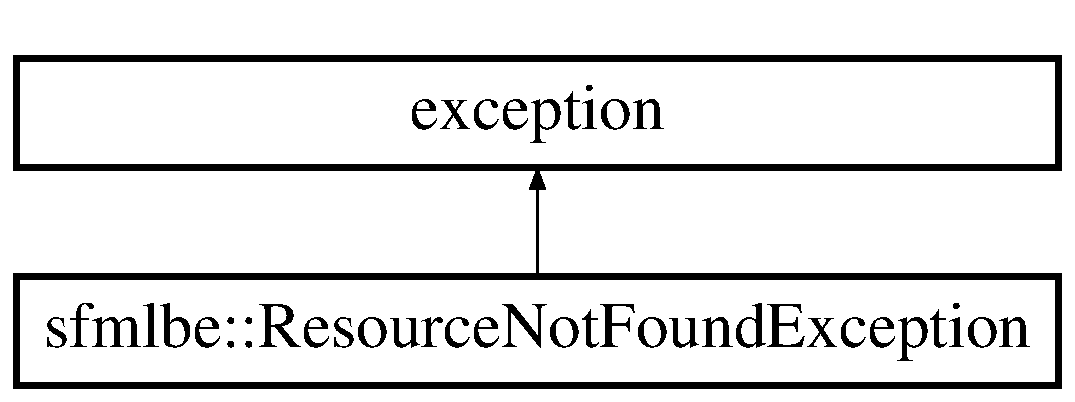
\includegraphics[height=2.000000cm]{classsfmlbe_1_1_resource_not_found_exception}
\end{center}
\end{figure}
\subsection*{Public Member Functions}
\begin{DoxyCompactItemize}
\item 
\mbox{\Hypertarget{classsfmlbe_1_1_resource_not_found_exception_a1ee8f9376a6f12829aa99a215b0eedb9}\label{classsfmlbe_1_1_resource_not_found_exception_a1ee8f9376a6f12829aa99a215b0eedb9}} 
{\bfseries Resource\+Not\+Found\+Exception} (const char $\ast$key)
\item 
\mbox{\Hypertarget{classsfmlbe_1_1_resource_not_found_exception_a9c7b4daf44b4054c4fcc4f9da223e0a9}\label{classsfmlbe_1_1_resource_not_found_exception_a9c7b4daf44b4054c4fcc4f9da223e0a9}} 
virtual const char $\ast$ {\bfseries what} () const  throw ()
\end{DoxyCompactItemize}


\subsection{Detailed Description}
Exception thrown when a sfmlbe\+::\+Ressource is not found in the resource map. 

The documentation for this class was generated from the following file\+:\begin{DoxyCompactItemize}
\item 
dev/header/\mbox{\hyperlink{resourceexceptions_8hpp}{resourceexceptions.\+hpp}}\end{DoxyCompactItemize}

\hypertarget{classsfmlbe_1_1_resource_not_load_exception}{}\section{sfmlbe\+:\+:Resource\+Not\+Load\+Exception Class Reference}
\label{classsfmlbe_1_1_resource_not_load_exception}\index{sfmlbe\+::\+Resource\+Not\+Load\+Exception@{sfmlbe\+::\+Resource\+Not\+Load\+Exception}}


{\ttfamily \#include $<$resourceexceptions.\+hpp$>$}

Inheritance diagram for sfmlbe\+:\+:Resource\+Not\+Load\+Exception\+:\begin{figure}[H]
\begin{center}
\leavevmode
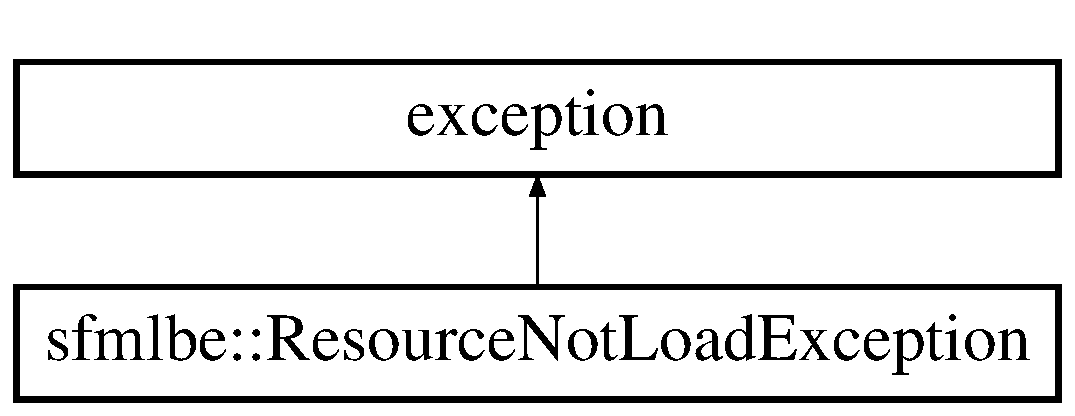
\includegraphics[height=2.000000cm]{classsfmlbe_1_1_resource_not_load_exception}
\end{center}
\end{figure}
\subsection*{Public Member Functions}
\begin{DoxyCompactItemize}
\item 
\mbox{\Hypertarget{classsfmlbe_1_1_resource_not_load_exception_adf8ded3c4b7fd9711064f737970bdf49}\label{classsfmlbe_1_1_resource_not_load_exception_adf8ded3c4b7fd9711064f737970bdf49}} 
{\bfseries Resource\+Not\+Load\+Exception} (const char $\ast$filename)
\item 
\mbox{\Hypertarget{classsfmlbe_1_1_resource_not_load_exception_a9c444cf9637f07bf7b80353f9a2032d9}\label{classsfmlbe_1_1_resource_not_load_exception_a9c444cf9637f07bf7b80353f9a2032d9}} 
virtual const char $\ast$ {\bfseries what} () const  throw ()
\end{DoxyCompactItemize}


\subsection{Detailed Description}
Exception thrown when a sfmlbe\+::\+Ressource is not loaded and should have been loaded. 

The documentation for this class was generated from the following file\+:\begin{DoxyCompactItemize}
\item 
dev/header/\mbox{\hyperlink{resourceexceptions_8hpp}{resourceexceptions.\+hpp}}\end{DoxyCompactItemize}

\hypertarget{classsfmlbe_1_1_resource_sound_buffer}{}\section{sfmlbe\+:\+:Resource\+Sound\+Buffer Class Reference}
\label{classsfmlbe_1_1_resource_sound_buffer}\index{sfmlbe\+::\+Resource\+Sound\+Buffer@{sfmlbe\+::\+Resource\+Sound\+Buffer}}


{\ttfamily \#include $<$resourcesoundbuffer.\+hpp$>$}

Inheritance diagram for sfmlbe\+:\+:Resource\+Sound\+Buffer\+:\begin{figure}[H]
\begin{center}
\leavevmode
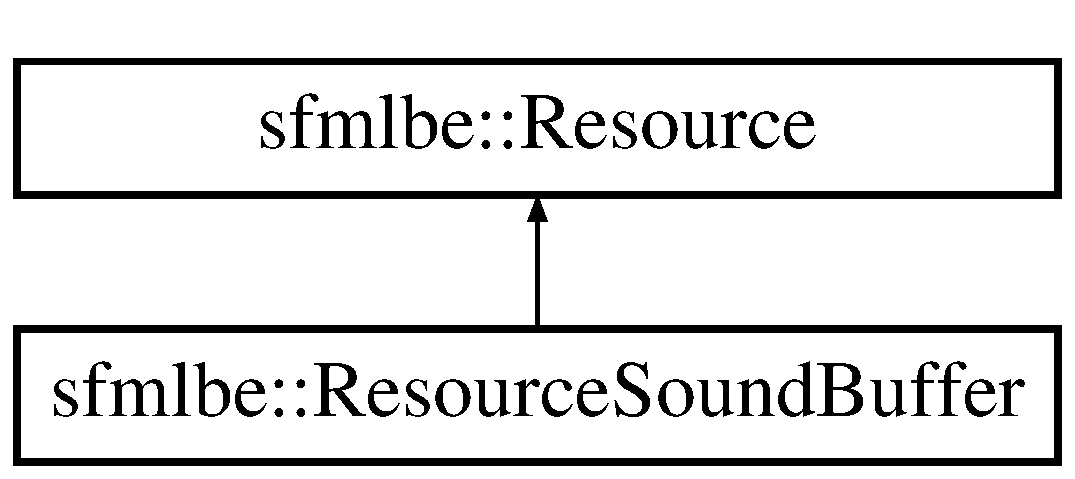
\includegraphics[height=2.000000cm]{classsfmlbe_1_1_resource_sound_buffer}
\end{center}
\end{figure}
\subsection*{Public Member Functions}
\begin{DoxyCompactItemize}
\item 
\mbox{\hyperlink{classsfmlbe_1_1_resource_sound_buffer_a88d7088f7f0e02879c0a62563851cb67}{Resource\+Sound\+Buffer}} ()
\begin{DoxyCompactList}\small\item\em Constructor. \end{DoxyCompactList}\item 
\mbox{\hyperlink{classsfmlbe_1_1_resource_sound_buffer_a6f01706abb7c87383e0ddffbf8650837}{Resource\+Sound\+Buffer}} (std\+::string ID, std\+::string filename)
\begin{DoxyCompactList}\small\item\em Constructor. \end{DoxyCompactList}\item 
\mbox{\hyperlink{classsfmlbe_1_1_resource_sound_buffer_a28e17a59ffd9de59eb6394ed564efc11}{$\sim$\+Resource\+Sound\+Buffer}} ()
\begin{DoxyCompactList}\small\item\em Descructor. \end{DoxyCompactList}\item 
void \mbox{\hyperlink{classsfmlbe_1_1_resource_sound_buffer_a1207531bb0e5355f90cf4a7f67734555}{Load}} ()
\begin{DoxyCompactList}\small\item\em Load the sf\+::\+Sound\+Buffer targeted by this resource. \end{DoxyCompactList}\item 
void \mbox{\hyperlink{classsfmlbe_1_1_resource_sound_buffer_aea7707b97d4451935597671c0e162a7b}{Unload}} ()
\begin{DoxyCompactList}\small\item\em Unload the sf\+::\+Sound\+Buffer targeted by this resource. \end{DoxyCompactList}\item 
sf\+::\+Sound\+Buffer $\ast$ \mbox{\hyperlink{classsfmlbe_1_1_resource_sound_buffer_a56043b6124e92d99a25e7756022088cb}{Get\+Sound\+Buffer}} ()
\begin{DoxyCompactList}\small\item\em Get the sf\+::\+Sound\+Buffer associed to this resource. \end{DoxyCompactList}\end{DoxyCompactItemize}
\subsection*{Additional Inherited Members}


\subsection{Detailed Description}
Class allowing to store a sf\+::\+Sound\+Buffer using the S\+F\+M\+L\+BE \mbox{\hyperlink{classsfmlbe_1_1_resource}{Resource}} Manager system. Provide an interface to load and unload soundbuffer easily. 

\subsection{Constructor \& Destructor Documentation}
\mbox{\Hypertarget{classsfmlbe_1_1_resource_sound_buffer_a88d7088f7f0e02879c0a62563851cb67}\label{classsfmlbe_1_1_resource_sound_buffer_a88d7088f7f0e02879c0a62563851cb67}} 
\index{sfmlbe\+::\+Resource\+Sound\+Buffer@{sfmlbe\+::\+Resource\+Sound\+Buffer}!Resource\+Sound\+Buffer@{Resource\+Sound\+Buffer}}
\index{Resource\+Sound\+Buffer@{Resource\+Sound\+Buffer}!sfmlbe\+::\+Resource\+Sound\+Buffer@{sfmlbe\+::\+Resource\+Sound\+Buffer}}
\subsubsection{\texorpdfstring{Resource\+Sound\+Buffer()}{ResourceSoundBuffer()}\hspace{0.1cm}{\footnotesize\ttfamily [1/2]}}
{\footnotesize\ttfamily sfmlbe\+::\+Resource\+Sound\+Buffer\+::\+Resource\+Sound\+Buffer (\begin{DoxyParamCaption}{ }\end{DoxyParamCaption})}



Constructor. 

Construct a non loaded soundbuffer resource. \begin{DoxySeeAlso}{See also}
\mbox{\hyperlink{classsfmlbe_1_1_resource_sound_buffer_a6f01706abb7c87383e0ddffbf8650837}{Resource\+Sound\+Buffer(std\+::string I\+D, std\+::string filename)}} and \mbox{\hyperlink{classsfmlbe_1_1_resource_sound_buffer_a28e17a59ffd9de59eb6394ed564efc11}{$\sim$\+Resource\+Sound\+Buffer()}} 
\end{DoxySeeAlso}
\mbox{\Hypertarget{classsfmlbe_1_1_resource_sound_buffer_a6f01706abb7c87383e0ddffbf8650837}\label{classsfmlbe_1_1_resource_sound_buffer_a6f01706abb7c87383e0ddffbf8650837}} 
\index{sfmlbe\+::\+Resource\+Sound\+Buffer@{sfmlbe\+::\+Resource\+Sound\+Buffer}!Resource\+Sound\+Buffer@{Resource\+Sound\+Buffer}}
\index{Resource\+Sound\+Buffer@{Resource\+Sound\+Buffer}!sfmlbe\+::\+Resource\+Sound\+Buffer@{sfmlbe\+::\+Resource\+Sound\+Buffer}}
\subsubsection{\texorpdfstring{Resource\+Sound\+Buffer()}{ResourceSoundBuffer()}\hspace{0.1cm}{\footnotesize\ttfamily [2/2]}}
{\footnotesize\ttfamily sfmlbe\+::\+Resource\+Sound\+Buffer\+::\+Resource\+Sound\+Buffer (\begin{DoxyParamCaption}\item[{std\+::string}]{ID,  }\item[{std\+::string}]{filename }\end{DoxyParamCaption})}



Constructor. 

Construct a non loaded soundbuffer resource, but with provided parameters. 
\begin{DoxyParams}{Parameters}
{\em ID} & ID of the resource in the scope specified. \\
\hline
{\em filename} & Relative path of file from where the resource is loaded. \\
\hline
\end{DoxyParams}
\begin{DoxySeeAlso}{See also}
\mbox{\hyperlink{classsfmlbe_1_1_resource_sound_buffer_a88d7088f7f0e02879c0a62563851cb67}{Resource\+Sound\+Buffer()}} and \mbox{\hyperlink{classsfmlbe_1_1_resource_sound_buffer_a28e17a59ffd9de59eb6394ed564efc11}{$\sim$\+Resource\+Sound\+Buffer()}} 
\end{DoxySeeAlso}
\mbox{\Hypertarget{classsfmlbe_1_1_resource_sound_buffer_a28e17a59ffd9de59eb6394ed564efc11}\label{classsfmlbe_1_1_resource_sound_buffer_a28e17a59ffd9de59eb6394ed564efc11}} 
\index{sfmlbe\+::\+Resource\+Sound\+Buffer@{sfmlbe\+::\+Resource\+Sound\+Buffer}!````~Resource\+Sound\+Buffer@{$\sim$\+Resource\+Sound\+Buffer}}
\index{````~Resource\+Sound\+Buffer@{$\sim$\+Resource\+Sound\+Buffer}!sfmlbe\+::\+Resource\+Sound\+Buffer@{sfmlbe\+::\+Resource\+Sound\+Buffer}}
\subsubsection{\texorpdfstring{$\sim$\+Resource\+Sound\+Buffer()}{~ResourceSoundBuffer()}}
{\footnotesize\ttfamily sfmlbe\+::\+Resource\+Sound\+Buffer\+::$\sim$\+Resource\+Sound\+Buffer (\begin{DoxyParamCaption}{ }\end{DoxyParamCaption})}



Descructor. 

Free memory used by the sf\+::\+Sound\+Buffer and this resource. \begin{DoxySeeAlso}{See also}
\mbox{\hyperlink{classsfmlbe_1_1_resource_sound_buffer_a88d7088f7f0e02879c0a62563851cb67}{Resource\+Sound\+Buffer()}} and \mbox{\hyperlink{classsfmlbe_1_1_resource_sound_buffer_a6f01706abb7c87383e0ddffbf8650837}{Resource\+Sound\+Buffer(std\+::string I\+D, std\+::string filename)}} 
\end{DoxySeeAlso}


\subsection{Member Function Documentation}
\mbox{\Hypertarget{classsfmlbe_1_1_resource_sound_buffer_a56043b6124e92d99a25e7756022088cb}\label{classsfmlbe_1_1_resource_sound_buffer_a56043b6124e92d99a25e7756022088cb}} 
\index{sfmlbe\+::\+Resource\+Sound\+Buffer@{sfmlbe\+::\+Resource\+Sound\+Buffer}!Get\+Sound\+Buffer@{Get\+Sound\+Buffer}}
\index{Get\+Sound\+Buffer@{Get\+Sound\+Buffer}!sfmlbe\+::\+Resource\+Sound\+Buffer@{sfmlbe\+::\+Resource\+Sound\+Buffer}}
\subsubsection{\texorpdfstring{Get\+Sound\+Buffer()}{GetSoundBuffer()}}
{\footnotesize\ttfamily sf\+::\+Sound\+Buffer$\ast$ sfmlbe\+::\+Resource\+Sound\+Buffer\+::\+Get\+Sound\+Buffer (\begin{DoxyParamCaption}{ }\end{DoxyParamCaption})\hspace{0.3cm}{\ttfamily [inline]}}



Get the sf\+::\+Sound\+Buffer associed to this resource. 

\begin{DoxyReturn}{Returns}
Reference to the sf\+::\+Sound\+Buffer or N\+U\+LL. 
\end{DoxyReturn}
\mbox{\Hypertarget{classsfmlbe_1_1_resource_sound_buffer_a1207531bb0e5355f90cf4a7f67734555}\label{classsfmlbe_1_1_resource_sound_buffer_a1207531bb0e5355f90cf4a7f67734555}} 
\index{sfmlbe\+::\+Resource\+Sound\+Buffer@{sfmlbe\+::\+Resource\+Sound\+Buffer}!Load@{Load}}
\index{Load@{Load}!sfmlbe\+::\+Resource\+Sound\+Buffer@{sfmlbe\+::\+Resource\+Sound\+Buffer}}
\subsubsection{\texorpdfstring{Load()}{Load()}}
{\footnotesize\ttfamily void sfmlbe\+::\+Resource\+Sound\+Buffer\+::\+Load (\begin{DoxyParamCaption}{ }\end{DoxyParamCaption})\hspace{0.3cm}{\ttfamily [virtual]}}



Load the sf\+::\+Sound\+Buffer targeted by this resource. 

If success set this resource as loaded. \begin{DoxySeeAlso}{See also}
\mbox{\hyperlink{classsfmlbe_1_1_resource_sound_buffer_aea7707b97d4451935597671c0e162a7b}{Unload()}} and \mbox{\hyperlink{classsfmlbe_1_1_resource_acd0812c81f7d5d851a4671f0cf7bb4f1}{Is\+Loaded()}} 
\end{DoxySeeAlso}


Implements \mbox{\hyperlink{classsfmlbe_1_1_resource_a35981869a1e90ebbf30258ff7aa1d6d2}{sfmlbe\+::\+Resource}}.

\mbox{\Hypertarget{classsfmlbe_1_1_resource_sound_buffer_aea7707b97d4451935597671c0e162a7b}\label{classsfmlbe_1_1_resource_sound_buffer_aea7707b97d4451935597671c0e162a7b}} 
\index{sfmlbe\+::\+Resource\+Sound\+Buffer@{sfmlbe\+::\+Resource\+Sound\+Buffer}!Unload@{Unload}}
\index{Unload@{Unload}!sfmlbe\+::\+Resource\+Sound\+Buffer@{sfmlbe\+::\+Resource\+Sound\+Buffer}}
\subsubsection{\texorpdfstring{Unload()}{Unload()}}
{\footnotesize\ttfamily void sfmlbe\+::\+Resource\+Sound\+Buffer\+::\+Unload (\begin{DoxyParamCaption}{ }\end{DoxyParamCaption})\hspace{0.3cm}{\ttfamily [virtual]}}



Unload the sf\+::\+Sound\+Buffer targeted by this resource. 

If success set this resource as unloaded. \begin{DoxySeeAlso}{See also}
\mbox{\hyperlink{classsfmlbe_1_1_resource_sound_buffer_a1207531bb0e5355f90cf4a7f67734555}{Load()}} and \mbox{\hyperlink{classsfmlbe_1_1_resource_acd0812c81f7d5d851a4671f0cf7bb4f1}{Is\+Loaded()}} 
\end{DoxySeeAlso}


Implements \mbox{\hyperlink{classsfmlbe_1_1_resource_a48c75a88679cf457965dd013f47014b9}{sfmlbe\+::\+Resource}}.



The documentation for this class was generated from the following file\+:\begin{DoxyCompactItemize}
\item 
dev/header/\mbox{\hyperlink{resourcesoundbuffer_8hpp}{resourcesoundbuffer.\+hpp}}\end{DoxyCompactItemize}

\hypertarget{classsfmlbe_1_1_resource_text}{}\section{sfmlbe\+:\+:Resource\+Text Class Reference}
\label{classsfmlbe_1_1_resource_text}\index{sfmlbe\+::\+Resource\+Text@{sfmlbe\+::\+Resource\+Text}}


{\ttfamily \#include $<$resourcetext.\+hpp$>$}

Inheritance diagram for sfmlbe\+:\+:Resource\+Text\+:\begin{figure}[H]
\begin{center}
\leavevmode
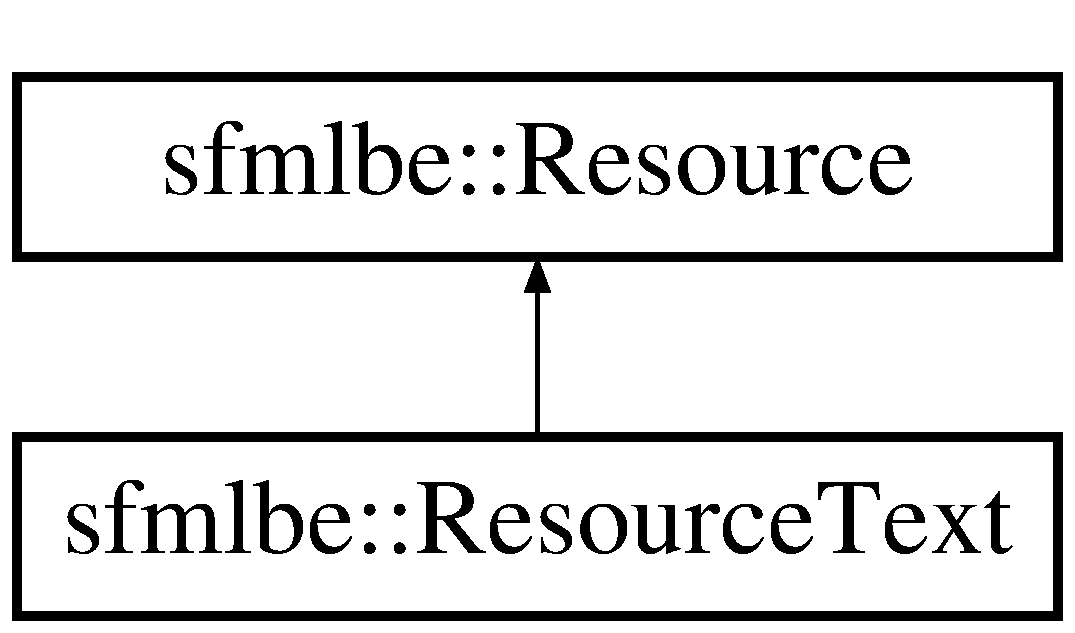
\includegraphics[height=2.000000cm]{classsfmlbe_1_1_resource_text}
\end{center}
\end{figure}
\subsection*{Public Member Functions}
\begin{DoxyCompactItemize}
\item 
\mbox{\hyperlink{classsfmlbe_1_1_resource_text_aaf976bc4d8e514a621239ab3ef61b294}{Resource\+Text}} ()
\begin{DoxyCompactList}\small\item\em Constructor. \end{DoxyCompactList}\item 
\mbox{\hyperlink{classsfmlbe_1_1_resource_text_a05e07dcbb416cee62e4060627a76c749}{Resource\+Text}} (std\+::string ID, std\+::string filename)
\begin{DoxyCompactList}\small\item\em Constructor. \end{DoxyCompactList}\item 
\mbox{\hyperlink{classsfmlbe_1_1_resource_text_a037b1bd5ac566301358ee5cd75a4cd00}{$\sim$\+Resource\+Text}} ()
\begin{DoxyCompactList}\small\item\em Descructor. \end{DoxyCompactList}\item 
void \mbox{\hyperlink{classsfmlbe_1_1_resource_text_a1176965f3e9d26c618688f7899b4b58b}{Load}} ()
\begin{DoxyCompactList}\small\item\em Load the std\+::map of the std\+::string targeted by this resource. \end{DoxyCompactList}\item 
void \mbox{\hyperlink{classsfmlbe_1_1_resource_text_a7493d044dfcd376b0fd17fd5fbd52ada}{Unload}} ()
\begin{DoxyCompactList}\small\item\em Unload the std\+::map of the std\+::string targeted by this resource. \end{DoxyCompactList}\item 
std\+::string $\ast$ \mbox{\hyperlink{classsfmlbe_1_1_resource_text_a36954e8d61e7406f4923fda6acd4e4f3}{Get\+Text}} (std\+::string key)
\begin{DoxyCompactList}\small\item\em Get the std\+::map of the std\+::string associed to this resource, with a key needed. \end{DoxyCompactList}\end{DoxyCompactItemize}
\subsection*{Additional Inherited Members}


\subsection{Detailed Description}
Class allowing to store a std\+::map of std\+::string using the S\+F\+M\+L\+BE \mbox{\hyperlink{classsfmlbe_1_1_resource}{Resource}} Manager system. Provide an interface to load and unload large texts easily. 

\subsection{Constructor \& Destructor Documentation}
\mbox{\Hypertarget{classsfmlbe_1_1_resource_text_aaf976bc4d8e514a621239ab3ef61b294}\label{classsfmlbe_1_1_resource_text_aaf976bc4d8e514a621239ab3ef61b294}} 
\index{sfmlbe\+::\+Resource\+Text@{sfmlbe\+::\+Resource\+Text}!Resource\+Text@{Resource\+Text}}
\index{Resource\+Text@{Resource\+Text}!sfmlbe\+::\+Resource\+Text@{sfmlbe\+::\+Resource\+Text}}
\subsubsection{\texorpdfstring{Resource\+Text()}{ResourceText()}\hspace{0.1cm}{\footnotesize\ttfamily [1/2]}}
{\footnotesize\ttfamily sfmlbe\+::\+Resource\+Text\+::\+Resource\+Text (\begin{DoxyParamCaption}{ }\end{DoxyParamCaption})}



Constructor. 

Construct a non loaded text resource. \begin{DoxySeeAlso}{See also}
\mbox{\hyperlink{classsfmlbe_1_1_resource_text_a05e07dcbb416cee62e4060627a76c749}{Resource\+Text(std\+::string I\+D, std\+::string filename)}} and \mbox{\hyperlink{classsfmlbe_1_1_resource_text_a037b1bd5ac566301358ee5cd75a4cd00}{$\sim$\+Resource\+Text()}} 
\end{DoxySeeAlso}
\mbox{\Hypertarget{classsfmlbe_1_1_resource_text_a05e07dcbb416cee62e4060627a76c749}\label{classsfmlbe_1_1_resource_text_a05e07dcbb416cee62e4060627a76c749}} 
\index{sfmlbe\+::\+Resource\+Text@{sfmlbe\+::\+Resource\+Text}!Resource\+Text@{Resource\+Text}}
\index{Resource\+Text@{Resource\+Text}!sfmlbe\+::\+Resource\+Text@{sfmlbe\+::\+Resource\+Text}}
\subsubsection{\texorpdfstring{Resource\+Text()}{ResourceText()}\hspace{0.1cm}{\footnotesize\ttfamily [2/2]}}
{\footnotesize\ttfamily sfmlbe\+::\+Resource\+Text\+::\+Resource\+Text (\begin{DoxyParamCaption}\item[{std\+::string}]{ID,  }\item[{std\+::string}]{filename }\end{DoxyParamCaption})}



Constructor. 

Construct a non loaded text resource, but with provided parameters. 
\begin{DoxyParams}{Parameters}
{\em ID} & ID of the resource in the scope specified. \\
\hline
{\em filename} & Relative path of file from where the resource is loaded. \\
\hline
\end{DoxyParams}
\begin{DoxySeeAlso}{See also}
\mbox{\hyperlink{classsfmlbe_1_1_resource_text_aaf976bc4d8e514a621239ab3ef61b294}{Resource\+Text()}} and \mbox{\hyperlink{classsfmlbe_1_1_resource_text_a037b1bd5ac566301358ee5cd75a4cd00}{$\sim$\+Resource\+Text()}} 
\end{DoxySeeAlso}
\mbox{\Hypertarget{classsfmlbe_1_1_resource_text_a037b1bd5ac566301358ee5cd75a4cd00}\label{classsfmlbe_1_1_resource_text_a037b1bd5ac566301358ee5cd75a4cd00}} 
\index{sfmlbe\+::\+Resource\+Text@{sfmlbe\+::\+Resource\+Text}!````~Resource\+Text@{$\sim$\+Resource\+Text}}
\index{````~Resource\+Text@{$\sim$\+Resource\+Text}!sfmlbe\+::\+Resource\+Text@{sfmlbe\+::\+Resource\+Text}}
\subsubsection{\texorpdfstring{$\sim$\+Resource\+Text()}{~ResourceText()}}
{\footnotesize\ttfamily sfmlbe\+::\+Resource\+Text\+::$\sim$\+Resource\+Text (\begin{DoxyParamCaption}{ }\end{DoxyParamCaption})}



Descructor. 

Free memory used by all the strings and this resource. \begin{DoxySeeAlso}{See also}
\mbox{\hyperlink{classsfmlbe_1_1_resource_text_aaf976bc4d8e514a621239ab3ef61b294}{Resource\+Text()}} and \mbox{\hyperlink{classsfmlbe_1_1_resource_text_a05e07dcbb416cee62e4060627a76c749}{Resource\+Text(std\+::string I\+D, std\+::string filename)}} 
\end{DoxySeeAlso}


\subsection{Member Function Documentation}
\mbox{\Hypertarget{classsfmlbe_1_1_resource_text_a36954e8d61e7406f4923fda6acd4e4f3}\label{classsfmlbe_1_1_resource_text_a36954e8d61e7406f4923fda6acd4e4f3}} 
\index{sfmlbe\+::\+Resource\+Text@{sfmlbe\+::\+Resource\+Text}!Get\+Text@{Get\+Text}}
\index{Get\+Text@{Get\+Text}!sfmlbe\+::\+Resource\+Text@{sfmlbe\+::\+Resource\+Text}}
\subsubsection{\texorpdfstring{Get\+Text()}{GetText()}}
{\footnotesize\ttfamily std\+::string$\ast$ sfmlbe\+::\+Resource\+Text\+::\+Get\+Text (\begin{DoxyParamCaption}\item[{std\+::string}]{key }\end{DoxyParamCaption})}



Get the std\+::map of the std\+::string associed to this resource, with a key needed. 


\begin{DoxyParams}{Parameters}
{\em key} & Key of the std\+::string wanted. \\
\hline
\end{DoxyParams}
\begin{DoxyReturn}{Returns}
Reference to the sf\+::map or N\+U\+LL. 
\end{DoxyReturn}
\mbox{\Hypertarget{classsfmlbe_1_1_resource_text_a1176965f3e9d26c618688f7899b4b58b}\label{classsfmlbe_1_1_resource_text_a1176965f3e9d26c618688f7899b4b58b}} 
\index{sfmlbe\+::\+Resource\+Text@{sfmlbe\+::\+Resource\+Text}!Load@{Load}}
\index{Load@{Load}!sfmlbe\+::\+Resource\+Text@{sfmlbe\+::\+Resource\+Text}}
\subsubsection{\texorpdfstring{Load()}{Load()}}
{\footnotesize\ttfamily void sfmlbe\+::\+Resource\+Text\+::\+Load (\begin{DoxyParamCaption}{ }\end{DoxyParamCaption})\hspace{0.3cm}{\ttfamily [virtual]}}



Load the std\+::map of the std\+::string targeted by this resource. 

If success set this resource as loaded. \begin{DoxySeeAlso}{See also}
\mbox{\hyperlink{classsfmlbe_1_1_resource_text_a7493d044dfcd376b0fd17fd5fbd52ada}{Unload()}} and \mbox{\hyperlink{classsfmlbe_1_1_resource_acd0812c81f7d5d851a4671f0cf7bb4f1}{Is\+Loaded()}} 
\end{DoxySeeAlso}


Implements \mbox{\hyperlink{classsfmlbe_1_1_resource_a35981869a1e90ebbf30258ff7aa1d6d2}{sfmlbe\+::\+Resource}}.

\mbox{\Hypertarget{classsfmlbe_1_1_resource_text_a7493d044dfcd376b0fd17fd5fbd52ada}\label{classsfmlbe_1_1_resource_text_a7493d044dfcd376b0fd17fd5fbd52ada}} 
\index{sfmlbe\+::\+Resource\+Text@{sfmlbe\+::\+Resource\+Text}!Unload@{Unload}}
\index{Unload@{Unload}!sfmlbe\+::\+Resource\+Text@{sfmlbe\+::\+Resource\+Text}}
\subsubsection{\texorpdfstring{Unload()}{Unload()}}
{\footnotesize\ttfamily void sfmlbe\+::\+Resource\+Text\+::\+Unload (\begin{DoxyParamCaption}{ }\end{DoxyParamCaption})\hspace{0.3cm}{\ttfamily [virtual]}}



Unload the std\+::map of the std\+::string targeted by this resource. 

If success set this resource as unloaded. \begin{DoxySeeAlso}{See also}
\mbox{\hyperlink{classsfmlbe_1_1_resource_text_a1176965f3e9d26c618688f7899b4b58b}{Load()}} and \mbox{\hyperlink{classsfmlbe_1_1_resource_acd0812c81f7d5d851a4671f0cf7bb4f1}{Is\+Loaded()}} 
\end{DoxySeeAlso}


Implements \mbox{\hyperlink{classsfmlbe_1_1_resource_a48c75a88679cf457965dd013f47014b9}{sfmlbe\+::\+Resource}}.



The documentation for this class was generated from the following file\+:\begin{DoxyCompactItemize}
\item 
dev/header/\mbox{\hyperlink{resourcetext_8hpp}{resourcetext.\+hpp}}\end{DoxyCompactItemize}

\hypertarget{classsfmlbe_1_1_resource_texture}{}\section{sfmlbe\+:\+:Resource\+Texture Class Reference}
\label{classsfmlbe_1_1_resource_texture}\index{sfmlbe\+::\+Resource\+Texture@{sfmlbe\+::\+Resource\+Texture}}


{\ttfamily \#include $<$resourcetexture.\+hpp$>$}

Inheritance diagram for sfmlbe\+:\+:Resource\+Texture\+:\begin{figure}[H]
\begin{center}
\leavevmode
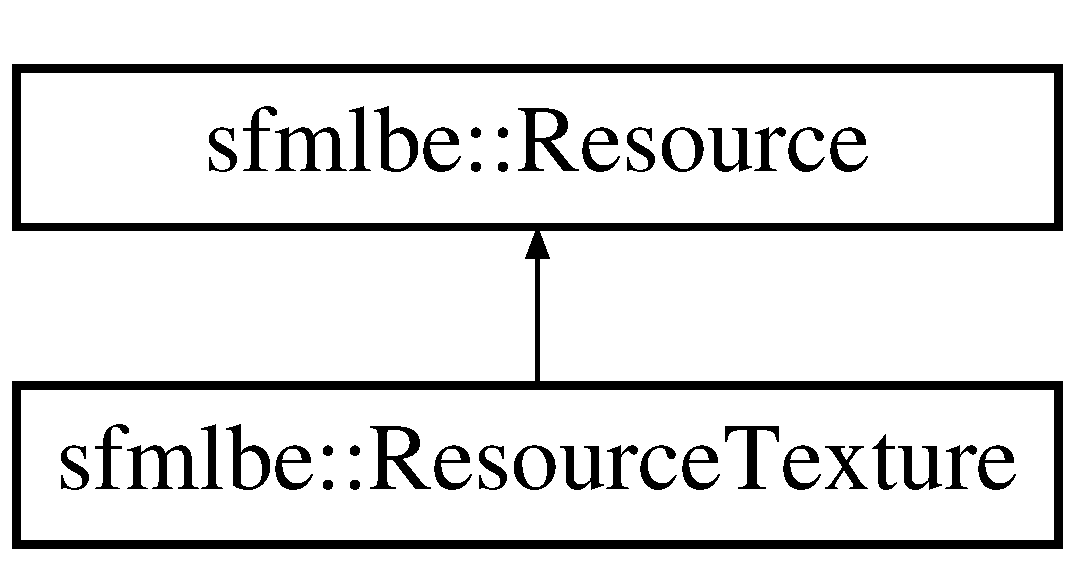
\includegraphics[height=2.000000cm]{classsfmlbe_1_1_resource_texture}
\end{center}
\end{figure}
\subsection*{Public Member Functions}
\begin{DoxyCompactItemize}
\item 
\mbox{\hyperlink{classsfmlbe_1_1_resource_texture_aa1a489c8fe125057b3009f6615093118}{Resource\+Texture}} ()
\begin{DoxyCompactList}\small\item\em Constructor. \end{DoxyCompactList}\item 
\mbox{\hyperlink{classsfmlbe_1_1_resource_texture_a458e1b22fd5074534d86f2665637ae34}{Resource\+Texture}} (std\+::string ID, std\+::string filename)
\begin{DoxyCompactList}\small\item\em Constructor. \end{DoxyCompactList}\item 
\mbox{\hyperlink{classsfmlbe_1_1_resource_texture_a98789b46742a42adffffe0abed982184}{$\sim$\+Resource\+Texture}} ()
\begin{DoxyCompactList}\small\item\em Descructor. \end{DoxyCompactList}\item 
void \mbox{\hyperlink{classsfmlbe_1_1_resource_texture_a4f8d27c8e50efce6d66a30edb078e2d3}{Load}} ()
\begin{DoxyCompactList}\small\item\em Load the sf\+::\+Texture targeted by this resource. \end{DoxyCompactList}\item 
void \mbox{\hyperlink{classsfmlbe_1_1_resource_texture_ac8b1b5866242e222abf0385144711646}{Unload}} ()
\begin{DoxyCompactList}\small\item\em Unload the sf\+::\+Texture targeted by this resource. \end{DoxyCompactList}\item 
sf\+::\+Texture $\ast$ \mbox{\hyperlink{classsfmlbe_1_1_resource_texture_a354d8f497b1ea0ca39c467219edc76c7}{Get\+Texture}} ()
\begin{DoxyCompactList}\small\item\em Get the sf\+::\+Texture associed to this resource. \end{DoxyCompactList}\end{DoxyCompactItemize}
\subsection*{Additional Inherited Members}


\subsection{Detailed Description}
Class allowing to store a sf\+::\+Texture using the S\+F\+M\+L\+BE \mbox{\hyperlink{classsfmlbe_1_1_resource}{Resource}} Manager system. Provide an interface to load and unload texture easily. 

\subsection{Constructor \& Destructor Documentation}
\mbox{\Hypertarget{classsfmlbe_1_1_resource_texture_aa1a489c8fe125057b3009f6615093118}\label{classsfmlbe_1_1_resource_texture_aa1a489c8fe125057b3009f6615093118}} 
\index{sfmlbe\+::\+Resource\+Texture@{sfmlbe\+::\+Resource\+Texture}!Resource\+Texture@{Resource\+Texture}}
\index{Resource\+Texture@{Resource\+Texture}!sfmlbe\+::\+Resource\+Texture@{sfmlbe\+::\+Resource\+Texture}}
\subsubsection{\texorpdfstring{Resource\+Texture()}{ResourceTexture()}\hspace{0.1cm}{\footnotesize\ttfamily [1/2]}}
{\footnotesize\ttfamily sfmlbe\+::\+Resource\+Texture\+::\+Resource\+Texture (\begin{DoxyParamCaption}{ }\end{DoxyParamCaption})}



Constructor. 

Construct a non loaded texture resource. \begin{DoxySeeAlso}{See also}
\mbox{\hyperlink{classsfmlbe_1_1_resource_texture_a458e1b22fd5074534d86f2665637ae34}{Resource\+Texture(std\+::string I\+D, std\+::string filename)}} and \mbox{\hyperlink{classsfmlbe_1_1_resource_texture_a98789b46742a42adffffe0abed982184}{$\sim$\+Resource\+Texture()}} 
\end{DoxySeeAlso}
\mbox{\Hypertarget{classsfmlbe_1_1_resource_texture_a458e1b22fd5074534d86f2665637ae34}\label{classsfmlbe_1_1_resource_texture_a458e1b22fd5074534d86f2665637ae34}} 
\index{sfmlbe\+::\+Resource\+Texture@{sfmlbe\+::\+Resource\+Texture}!Resource\+Texture@{Resource\+Texture}}
\index{Resource\+Texture@{Resource\+Texture}!sfmlbe\+::\+Resource\+Texture@{sfmlbe\+::\+Resource\+Texture}}
\subsubsection{\texorpdfstring{Resource\+Texture()}{ResourceTexture()}\hspace{0.1cm}{\footnotesize\ttfamily [2/2]}}
{\footnotesize\ttfamily sfmlbe\+::\+Resource\+Texture\+::\+Resource\+Texture (\begin{DoxyParamCaption}\item[{std\+::string}]{ID,  }\item[{std\+::string}]{filename }\end{DoxyParamCaption})}



Constructor. 

Construct a non loaded texture resource, but with provided parameters. 
\begin{DoxyParams}{Parameters}
{\em ID} & ID of the resource in the scope specified. \\
\hline
{\em filename} & Relative path of file from where the resource is loaded. \\
\hline
\end{DoxyParams}
\begin{DoxySeeAlso}{See also}
\mbox{\hyperlink{classsfmlbe_1_1_resource_texture_aa1a489c8fe125057b3009f6615093118}{Resource\+Texture()}} and \mbox{\hyperlink{classsfmlbe_1_1_resource_texture_a98789b46742a42adffffe0abed982184}{$\sim$\+Resource\+Texture()}} 
\end{DoxySeeAlso}
\mbox{\Hypertarget{classsfmlbe_1_1_resource_texture_a98789b46742a42adffffe0abed982184}\label{classsfmlbe_1_1_resource_texture_a98789b46742a42adffffe0abed982184}} 
\index{sfmlbe\+::\+Resource\+Texture@{sfmlbe\+::\+Resource\+Texture}!````~Resource\+Texture@{$\sim$\+Resource\+Texture}}
\index{````~Resource\+Texture@{$\sim$\+Resource\+Texture}!sfmlbe\+::\+Resource\+Texture@{sfmlbe\+::\+Resource\+Texture}}
\subsubsection{\texorpdfstring{$\sim$\+Resource\+Texture()}{~ResourceTexture()}}
{\footnotesize\ttfamily sfmlbe\+::\+Resource\+Texture\+::$\sim$\+Resource\+Texture (\begin{DoxyParamCaption}{ }\end{DoxyParamCaption})}



Descructor. 

Free memory used by the sf\+::\+Texture and this resource. \begin{DoxySeeAlso}{See also}
\mbox{\hyperlink{classsfmlbe_1_1_resource_texture_aa1a489c8fe125057b3009f6615093118}{Resource\+Texture()}} and \mbox{\hyperlink{classsfmlbe_1_1_resource_texture_a458e1b22fd5074534d86f2665637ae34}{Resource\+Texture(std\+::string I\+D, std\+::string filename)}} 
\end{DoxySeeAlso}


\subsection{Member Function Documentation}
\mbox{\Hypertarget{classsfmlbe_1_1_resource_texture_a354d8f497b1ea0ca39c467219edc76c7}\label{classsfmlbe_1_1_resource_texture_a354d8f497b1ea0ca39c467219edc76c7}} 
\index{sfmlbe\+::\+Resource\+Texture@{sfmlbe\+::\+Resource\+Texture}!Get\+Texture@{Get\+Texture}}
\index{Get\+Texture@{Get\+Texture}!sfmlbe\+::\+Resource\+Texture@{sfmlbe\+::\+Resource\+Texture}}
\subsubsection{\texorpdfstring{Get\+Texture()}{GetTexture()}}
{\footnotesize\ttfamily sf\+::\+Texture$\ast$ sfmlbe\+::\+Resource\+Texture\+::\+Get\+Texture (\begin{DoxyParamCaption}{ }\end{DoxyParamCaption})\hspace{0.3cm}{\ttfamily [inline]}}



Get the sf\+::\+Texture associed to this resource. 

\begin{DoxyReturn}{Returns}
Reference to the sf\+::\+Texture or N\+U\+LL. 
\end{DoxyReturn}
\mbox{\Hypertarget{classsfmlbe_1_1_resource_texture_a4f8d27c8e50efce6d66a30edb078e2d3}\label{classsfmlbe_1_1_resource_texture_a4f8d27c8e50efce6d66a30edb078e2d3}} 
\index{sfmlbe\+::\+Resource\+Texture@{sfmlbe\+::\+Resource\+Texture}!Load@{Load}}
\index{Load@{Load}!sfmlbe\+::\+Resource\+Texture@{sfmlbe\+::\+Resource\+Texture}}
\subsubsection{\texorpdfstring{Load()}{Load()}}
{\footnotesize\ttfamily void sfmlbe\+::\+Resource\+Texture\+::\+Load (\begin{DoxyParamCaption}{ }\end{DoxyParamCaption})\hspace{0.3cm}{\ttfamily [virtual]}}



Load the sf\+::\+Texture targeted by this resource. 

If success set this resource as loaded. \begin{DoxySeeAlso}{See also}
\mbox{\hyperlink{classsfmlbe_1_1_resource_texture_ac8b1b5866242e222abf0385144711646}{Unload()}} and \mbox{\hyperlink{classsfmlbe_1_1_resource_acd0812c81f7d5d851a4671f0cf7bb4f1}{Is\+Loaded()}} 
\end{DoxySeeAlso}


Implements \mbox{\hyperlink{classsfmlbe_1_1_resource_a35981869a1e90ebbf30258ff7aa1d6d2}{sfmlbe\+::\+Resource}}.

\mbox{\Hypertarget{classsfmlbe_1_1_resource_texture_ac8b1b5866242e222abf0385144711646}\label{classsfmlbe_1_1_resource_texture_ac8b1b5866242e222abf0385144711646}} 
\index{sfmlbe\+::\+Resource\+Texture@{sfmlbe\+::\+Resource\+Texture}!Unload@{Unload}}
\index{Unload@{Unload}!sfmlbe\+::\+Resource\+Texture@{sfmlbe\+::\+Resource\+Texture}}
\subsubsection{\texorpdfstring{Unload()}{Unload()}}
{\footnotesize\ttfamily void sfmlbe\+::\+Resource\+Texture\+::\+Unload (\begin{DoxyParamCaption}{ }\end{DoxyParamCaption})\hspace{0.3cm}{\ttfamily [virtual]}}



Unload the sf\+::\+Texture targeted by this resource. 

If success set this resource as unloaded. \begin{DoxySeeAlso}{See also}
\mbox{\hyperlink{classsfmlbe_1_1_resource_texture_a4f8d27c8e50efce6d66a30edb078e2d3}{Load()}} and \mbox{\hyperlink{classsfmlbe_1_1_resource_acd0812c81f7d5d851a4671f0cf7bb4f1}{Is\+Loaded()}} 
\end{DoxySeeAlso}


Implements \mbox{\hyperlink{classsfmlbe_1_1_resource_a48c75a88679cf457965dd013f47014b9}{sfmlbe\+::\+Resource}}.



The documentation for this class was generated from the following file\+:\begin{DoxyCompactItemize}
\item 
dev/header/\mbox{\hyperlink{resourcetexture_8hpp}{resourcetexture.\+hpp}}\end{DoxyCompactItemize}

\hypertarget{classsfmlbe_1_1_scope_not_found_exception}{}\section{sfmlbe\+:\+:Scope\+Not\+Found\+Exception Class Reference}
\label{classsfmlbe_1_1_scope_not_found_exception}\index{sfmlbe\+::\+Scope\+Not\+Found\+Exception@{sfmlbe\+::\+Scope\+Not\+Found\+Exception}}


{\ttfamily \#include $<$resourceexceptions.\+hpp$>$}

Inheritance diagram for sfmlbe\+:\+:Scope\+Not\+Found\+Exception\+:\begin{figure}[H]
\begin{center}
\leavevmode
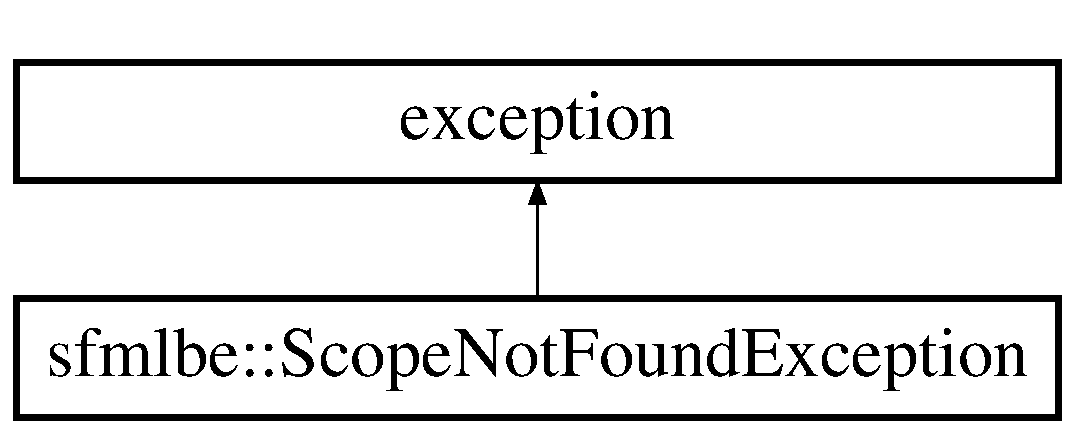
\includegraphics[height=2.000000cm]{classsfmlbe_1_1_scope_not_found_exception}
\end{center}
\end{figure}
\subsection*{Public Member Functions}
\begin{DoxyCompactItemize}
\item 
\mbox{\Hypertarget{classsfmlbe_1_1_scope_not_found_exception_aa27280e9efa824c4ca80103a3eeaa881}\label{classsfmlbe_1_1_scope_not_found_exception_aa27280e9efa824c4ca80103a3eeaa881}} 
{\bfseries Scope\+Not\+Found\+Exception} (const char $\ast$key)
\item 
\mbox{\Hypertarget{classsfmlbe_1_1_scope_not_found_exception_aa5a6fdb9880a3e3c8a573b6bd77440cb}\label{classsfmlbe_1_1_scope_not_found_exception_aa5a6fdb9880a3e3c8a573b6bd77440cb}} 
virtual const char $\ast$ {\bfseries what} () const  throw ()
\end{DoxyCompactItemize}


\subsection{Detailed Description}
Exception thrown when a scope is not found in the resource map. 

The documentation for this class was generated from the following file\+:\begin{DoxyCompactItemize}
\item 
dev/header/\mbox{\hyperlink{resourceexceptions_8hpp}{resourceexceptions.\+hpp}}\end{DoxyCompactItemize}

\hypertarget{classsfmlbe_1_1_singleton}{}\section{sfmlbe\+:\+:Singleton$<$ T $>$ Class Template Reference}
\label{classsfmlbe_1_1_singleton}\index{sfmlbe\+::\+Singleton$<$ T $>$@{sfmlbe\+::\+Singleton$<$ T $>$}}


{\ttfamily \#include $<$singleton.\+hpp$>$}

\subsection*{Static Public Member Functions}
\begin{DoxyCompactItemize}
\item 
static T $\ast$ \mbox{\hyperlink{classsfmlbe_1_1_singleton_a313529b2a097425bf5500df8848ead3e}{Get\+Instance}} ()
\item 
static void \mbox{\hyperlink{classsfmlbe_1_1_singleton_a0fa947a0f0940b94f757e49b56f37555}{Kill}} ()
\end{DoxyCompactItemize}
\subsection*{Protected Member Functions}
\begin{DoxyCompactItemize}
\item 
\mbox{\Hypertarget{classsfmlbe_1_1_singleton_a3f47ec090e5341446601408f9d38b467}\label{classsfmlbe_1_1_singleton_a3f47ec090e5341446601408f9d38b467}} 
\mbox{\hyperlink{classsfmlbe_1_1_singleton_a3f47ec090e5341446601408f9d38b467}{Singleton}} ()
\begin{DoxyCompactList}\small\item\em Constructor. \end{DoxyCompactList}\item 
\mbox{\Hypertarget{classsfmlbe_1_1_singleton_aa99901d754398a178b10e72fcc582b80}\label{classsfmlbe_1_1_singleton_aa99901d754398a178b10e72fcc582b80}} 
\mbox{\hyperlink{classsfmlbe_1_1_singleton_aa99901d754398a178b10e72fcc582b80}{$\sim$\+Singleton}} ()
\begin{DoxyCompactList}\small\item\em Destructor. \end{DoxyCompactList}\end{DoxyCompactItemize}


\subsection{Detailed Description}
\subsubsection*{template$<$typename T$>$\newline
class sfmlbe\+::\+Singleton$<$ T $>$}

Class representing a \mbox{\hyperlink{classsfmlbe_1_1_singleton}{Singleton}} pattern for a typename T. Used in \mbox{\hyperlink{classsfmlbe_1_1_resource_manager}{Resource\+Manager}}. Thread safe. 

\subsection{Member Function Documentation}
\mbox{\Hypertarget{classsfmlbe_1_1_singleton_a313529b2a097425bf5500df8848ead3e}\label{classsfmlbe_1_1_singleton_a313529b2a097425bf5500df8848ead3e}} 
\index{sfmlbe\+::\+Singleton@{sfmlbe\+::\+Singleton}!Get\+Instance@{Get\+Instance}}
\index{Get\+Instance@{Get\+Instance}!sfmlbe\+::\+Singleton@{sfmlbe\+::\+Singleton}}
\subsubsection{\texorpdfstring{Get\+Instance()}{GetInstance()}}
{\footnotesize\ttfamily template$<$typename T$>$ \\
static T$\ast$ \mbox{\hyperlink{classsfmlbe_1_1_singleton}{sfmlbe\+::\+Singleton}}$<$ T $>$\+::Get\+Instance (\begin{DoxyParamCaption}{ }\end{DoxyParamCaption})\hspace{0.3cm}{\ttfamily [inline]}, {\ttfamily [static]}}

Static function used to get a reference to the instance of the \mbox{\hyperlink{classsfmlbe_1_1_singleton}{Singleton}} templated class (thread safe). \mbox{\Hypertarget{classsfmlbe_1_1_singleton_a0fa947a0f0940b94f757e49b56f37555}\label{classsfmlbe_1_1_singleton_a0fa947a0f0940b94f757e49b56f37555}} 
\index{sfmlbe\+::\+Singleton@{sfmlbe\+::\+Singleton}!Kill@{Kill}}
\index{Kill@{Kill}!sfmlbe\+::\+Singleton@{sfmlbe\+::\+Singleton}}
\subsubsection{\texorpdfstring{Kill()}{Kill()}}
{\footnotesize\ttfamily template$<$typename T$>$ \\
static void \mbox{\hyperlink{classsfmlbe_1_1_singleton}{sfmlbe\+::\+Singleton}}$<$ T $>$\+::Kill (\begin{DoxyParamCaption}{ }\end{DoxyParamCaption})\hspace{0.3cm}{\ttfamily [inline]}, {\ttfamily [static]}}

Static function used to clear the memory and the reference to the instance of the \mbox{\hyperlink{classsfmlbe_1_1_singleton}{Singleton}} templated class. 

The documentation for this class was generated from the following file\+:\begin{DoxyCompactItemize}
\item 
dev/header/\mbox{\hyperlink{singleton_8hpp}{singleton.\+hpp}}\end{DoxyCompactItemize}

\chapter{File Documentation}
\hypertarget{common_8hpp}{}\section{dev/header/common.hpp File Reference}
\label{common_8hpp}\index{dev/header/common.\+hpp@{dev/header/common.\+hpp}}


Misc of component for S\+F\+M\+L\+BE.  


\subsection*{Namespaces}
\begin{DoxyCompactItemize}
\item 
 \mbox{\hyperlink{namespacesfmlbe}{sfmlbe}}
\end{DoxyCompactItemize}
\subsection*{Macros}
\begin{DoxyCompactItemize}
\item 
\#define \mbox{\hyperlink{common_8hpp_a91123955204178c3c47e9a46a73fe455}{\+\_\+\+G\+E\+T\+\_\+\+S\+O\+U\+N\+D\+B\+U\+F\+F\+ER}}(key)~((\mbox{\hyperlink{classsfmlbe_1_1_resource_sound_buffer}{sfmlbe\+::\+Resource\+Sound\+Buffer}} $\ast$)(\mbox{\hyperlink{classsfmlbe_1_1_singleton_a313529b2a097425bf5500df8848ead3e}{sfmlbe\+::\+Resource\+Manager\+::\+Get\+Instance}}()-\/$>$Find\+Resource\+By\+ID(key)))-\/$>$Get\+Sound\+Buffer()
\item 
\#define \mbox{\hyperlink{common_8hpp_acd56d2aebdf609d6d5ddbd1d31e85afc}{\+\_\+\+G\+E\+T\+\_\+\+S\+O\+U\+N\+D\+B\+U\+F\+F\+E\+R\+\_\+\+S\+C\+O\+PE}}(key,  scope)~((\mbox{\hyperlink{classsfmlbe_1_1_resource_sound_buffer}{sfmlbe\+::\+Resource\+Sound\+Buffer}} $\ast$)(\mbox{\hyperlink{classsfmlbe_1_1_singleton_a313529b2a097425bf5500df8848ead3e}{sfmlbe\+::\+Resource\+Manager\+::\+Get\+Instance}}()-\/$>$Find\+Resource\+By\+ID(key, scope)))-\/$>$Get\+Sound\+Buffer()
\item 
\#define \mbox{\hyperlink{common_8hpp_a6cb231e771687ec2365d07dbbc4ca84e}{\+\_\+\+G\+E\+T\+\_\+\+T\+E\+X\+T\+U\+RE}}(key)~((\mbox{\hyperlink{classsfmlbe_1_1_resource_texture}{sfmlbe\+::\+Resource\+Texture}} $\ast$)(\mbox{\hyperlink{classsfmlbe_1_1_singleton_a313529b2a097425bf5500df8848ead3e}{sfmlbe\+::\+Resource\+Manager\+::\+Get\+Instance}}()-\/$>$Find\+Resource\+By\+ID(key)))-\/$>$Get\+Texture()
\item 
\#define \mbox{\hyperlink{common_8hpp_a0c23c831a3c8c789dce76c32337c164f}{\+\_\+\+G\+E\+T\+\_\+\+T\+E\+X\+T\+U\+R\+E\+\_\+\+S\+C\+O\+PE}}(key,  scope)~((\mbox{\hyperlink{classsfmlbe_1_1_resource_texture}{sfmlbe\+::\+Resource\+Texture}} $\ast$)(\mbox{\hyperlink{classsfmlbe_1_1_singleton_a313529b2a097425bf5500df8848ead3e}{sfmlbe\+::\+Resource\+Manager\+::\+Get\+Instance}}()-\/$>$Find\+Resource\+By\+ID(key, scope)))-\/$>$Get\+Texture()
\item 
\#define \mbox{\hyperlink{common_8hpp_a8d8081f0d0ad6f79d654778d16870bca}{\+\_\+\+G\+E\+T\+\_\+\+M\+U\+S\+IC}}(key)~((\mbox{\hyperlink{classsfmlbe_1_1_resource_music}{sfmlbe\+::\+Resource\+Music}} $\ast$)(\mbox{\hyperlink{classsfmlbe_1_1_singleton_a313529b2a097425bf5500df8848ead3e}{sfmlbe\+::\+Resource\+Manager\+::\+Get\+Instance}}()-\/$>$Find\+Resource\+By\+ID(key)))-\/$>$Get\+Music()
\item 
\#define \mbox{\hyperlink{common_8hpp_aee599e12f9611ff5a4c5fe1de5d9e426}{\+\_\+\+G\+E\+T\+\_\+\+M\+U\+S\+I\+C\+\_\+\+S\+C\+O\+PE}}(key,  scope)~((\mbox{\hyperlink{classsfmlbe_1_1_resource_music}{sfmlbe\+::\+Resource\+Music}} $\ast$)(\mbox{\hyperlink{classsfmlbe_1_1_singleton_a313529b2a097425bf5500df8848ead3e}{sfmlbe\+::\+Resource\+Manager\+::\+Get\+Instance}}()-\/$>$Find\+Resource\+By\+ID(key, scope)))-\/$>$Get\+Music()
\item 
\#define \mbox{\hyperlink{common_8hpp_a171b5a386e18923861417af7b15ecdd7}{\+\_\+\+G\+E\+T\+\_\+\+F\+O\+NT}}(key)~((\mbox{\hyperlink{classsfmlbe_1_1_resource_font}{sfmlbe\+::\+Resource\+Font}} $\ast$)(\mbox{\hyperlink{classsfmlbe_1_1_singleton_a313529b2a097425bf5500df8848ead3e}{sfmlbe\+::\+Resource\+Manager\+::\+Get\+Instance}}()-\/$>$Find\+Resource\+By\+ID(key)))-\/$>$Get\+Font()
\item 
\#define \mbox{\hyperlink{common_8hpp_aded42a0ab80920668c19198ecdc5496b}{\+\_\+\+G\+E\+T\+\_\+\+F\+O\+N\+T\+\_\+\+S\+C\+O\+PE}}(key,  scope)~((\mbox{\hyperlink{classsfmlbe_1_1_resource_font}{sfmlbe\+::\+Resource\+Font}} $\ast$)(\mbox{\hyperlink{classsfmlbe_1_1_singleton_a313529b2a097425bf5500df8848ead3e}{sfmlbe\+::\+Resource\+Manager\+::\+Get\+Instance}}()-\/$>$Find\+Resource\+By\+ID(key, scope)))-\/$>$Get\+Font()
\item 
\#define \mbox{\hyperlink{common_8hpp_af75fcb1d120dd3bf410ba5461ffbcce1}{\+\_\+\+G\+E\+T\+\_\+\+T\+E\+XT}}(key,  key\+\_\+text)~((\mbox{\hyperlink{classsfmlbe_1_1_resource_text}{sfmlbe\+::\+Resource\+Text}} $\ast$)(\mbox{\hyperlink{classsfmlbe_1_1_singleton_a313529b2a097425bf5500df8848ead3e}{sfmlbe\+::\+Resource\+Manager\+::\+Get\+Instance}}()-\/$>$Find\+Resource\+By\+ID(key)))-\/$>$Get\+Text(key\+\_\+text)
\item 
\#define \mbox{\hyperlink{common_8hpp_a78fc8334e564d9cce24c83511f4b74d2}{\+\_\+\+G\+E\+T\+\_\+\+T\+E\+X\+T\+\_\+\+S\+C\+O\+PE}}(key,  scope,  key\+\_\+text)~((\mbox{\hyperlink{classsfmlbe_1_1_resource_text}{sfmlbe\+::\+Resource\+Text}} $\ast$)(\mbox{\hyperlink{classsfmlbe_1_1_singleton_a313529b2a097425bf5500df8848ead3e}{sfmlbe\+::\+Resource\+Manager\+::\+Get\+Instance}}()-\/$>$Find\+Resource\+By\+ID(key, scope)))-\/$>$Get\+Text(key\+\_\+text)
\end{DoxyCompactItemize}
\subsection*{Enumerations}
\begin{DoxyCompactItemize}
\item 
enum \mbox{\hyperlink{namespacesfmlbe_ac4335ed3060bba025f73e01f9dccb2dd}{sfmlbe\+::\+R\+E\+S\+O\+U\+R\+C\+E\+\_\+\+T\+Y\+PE}} \{ \newline
\mbox{\hyperlink{namespacesfmlbe_ac4335ed3060bba025f73e01f9dccb2dda8d19259bccf0ab6ee075b32fff6f7e54}{sfmlbe\+::\+R\+E\+S\+O\+U\+R\+C\+E\+\_\+\+N\+U\+LL}} = 0, 
\mbox{\hyperlink{namespacesfmlbe_ac4335ed3060bba025f73e01f9dccb2dda660c8cdfebf28528f6f0631ae29f89a5}{sfmlbe\+::\+R\+E\+S\+O\+U\+R\+C\+E\+\_\+\+G\+R\+A\+P\+H\+IC}} = 1, 
\mbox{\hyperlink{namespacesfmlbe_ac4335ed3060bba025f73e01f9dccb2dda06cb8047cf98a2679b83166ad27d2708}{sfmlbe\+::\+R\+E\+S\+O\+U\+R\+C\+E\+\_\+\+S\+O\+U\+N\+D\+B\+U\+F\+F\+ER}} = 2, 
\mbox{\hyperlink{namespacesfmlbe_ac4335ed3060bba025f73e01f9dccb2ddab44bcfdfdfd1fd38857b8ad914608007}{sfmlbe\+::\+R\+E\+S\+O\+U\+R\+C\+E\+\_\+\+M\+U\+S\+IC}} = 3, 
\newline
\mbox{\hyperlink{namespacesfmlbe_ac4335ed3060bba025f73e01f9dccb2dda9550a304907119d426805e6ed9a6c193}{sfmlbe\+::\+R\+E\+S\+O\+U\+R\+C\+E\+\_\+\+T\+E\+XT}} = 4, 
\mbox{\hyperlink{namespacesfmlbe_ac4335ed3060bba025f73e01f9dccb2dda7eae53eb53c90d3adcdfa9a16ebc34b7}{sfmlbe\+::\+R\+E\+S\+O\+U\+R\+C\+E\+\_\+\+F\+O\+NT}} = 5
 \}
\item 
enum \mbox{\hyperlink{namespacesfmlbe_add7861f7feda29864e1760490cd2eb15}{sfmlbe\+::\+L\+A\+NG}} \{ \mbox{\hyperlink{namespacesfmlbe_add7861f7feda29864e1760490cd2eb15aa40aa84e9e7799c8af50550a2ac17c38}{sfmlbe\+::\+EN}}, 
\mbox{\hyperlink{namespacesfmlbe_add7861f7feda29864e1760490cd2eb15ab5c87eb879bd8b0de0897fdc995ff17c}{sfmlbe\+::\+FR}}, 
\mbox{\hyperlink{namespacesfmlbe_add7861f7feda29864e1760490cd2eb15a3b7cf0aa10051afb9febea3f0c570495}{sfmlbe\+::\+DE}}, 
\mbox{\hyperlink{namespacesfmlbe_add7861f7feda29864e1760490cd2eb15ac4b5a57b91d3e35a463bb7ea672fadd2}{sfmlbe\+::\+SP}}
 \}
\end{DoxyCompactItemize}


\subsection{Detailed Description}
Misc of component for S\+F\+M\+L\+BE. 

\begin{DoxyAuthor}{Author}
Etienne Andrieu 
\end{DoxyAuthor}
\begin{DoxyVersion}{Version}
1.\+0 
\end{DoxyVersion}


\subsection{Macro Definition Documentation}
\mbox{\Hypertarget{common_8hpp_a171b5a386e18923861417af7b15ecdd7}\label{common_8hpp_a171b5a386e18923861417af7b15ecdd7}} 
\index{common.\+hpp@{common.\+hpp}!\+\_\+\+G\+E\+T\+\_\+\+F\+O\+NT@{\+\_\+\+G\+E\+T\+\_\+\+F\+O\+NT}}
\index{\+\_\+\+G\+E\+T\+\_\+\+F\+O\+NT@{\+\_\+\+G\+E\+T\+\_\+\+F\+O\+NT}!common.\+hpp@{common.\+hpp}}
\subsubsection{\texorpdfstring{\+\_\+\+G\+E\+T\+\_\+\+F\+O\+NT}{\_GET\_FONT}}
{\footnotesize\ttfamily \#define \+\_\+\+G\+E\+T\+\_\+\+F\+O\+NT(\begin{DoxyParamCaption}\item[{}]{key }\end{DoxyParamCaption})~((\mbox{\hyperlink{classsfmlbe_1_1_resource_font}{sfmlbe\+::\+Resource\+Font}} $\ast$)(\mbox{\hyperlink{classsfmlbe_1_1_singleton_a313529b2a097425bf5500df8848ead3e}{sfmlbe\+::\+Resource\+Manager\+::\+Get\+Instance}}()-\/$>$Find\+Resource\+By\+ID(key)))-\/$>$Get\+Font()}

Get the sfml\+::\+Font from a key. 
\begin{DoxyParams}{Parameters}
{\em key} & String used for ID to search the resource. \\
\hline
\end{DoxyParams}
\begin{DoxyReturn}{Returns}
First sfml\+::\+Font $\ast$ where the id equal to key. 
\end{DoxyReturn}

\begin{DoxyExceptions}{Exceptions}
{\em \mbox{\hyperlink{classsfmlbe_1_1_resource_not_found_exception}{sfmlbe\+::\+Resource\+Not\+Found\+Exception}}} & if the resource is not found in any scope. \\
\hline
\end{DoxyExceptions}
\mbox{\Hypertarget{common_8hpp_aded42a0ab80920668c19198ecdc5496b}\label{common_8hpp_aded42a0ab80920668c19198ecdc5496b}} 
\index{common.\+hpp@{common.\+hpp}!\+\_\+\+G\+E\+T\+\_\+\+F\+O\+N\+T\+\_\+\+S\+C\+O\+PE@{\+\_\+\+G\+E\+T\+\_\+\+F\+O\+N\+T\+\_\+\+S\+C\+O\+PE}}
\index{\+\_\+\+G\+E\+T\+\_\+\+F\+O\+N\+T\+\_\+\+S\+C\+O\+PE@{\+\_\+\+G\+E\+T\+\_\+\+F\+O\+N\+T\+\_\+\+S\+C\+O\+PE}!common.\+hpp@{common.\+hpp}}
\subsubsection{\texorpdfstring{\+\_\+\+G\+E\+T\+\_\+\+F\+O\+N\+T\+\_\+\+S\+C\+O\+PE}{\_GET\_FONT\_SCOPE}}
{\footnotesize\ttfamily \#define \+\_\+\+G\+E\+T\+\_\+\+F\+O\+N\+T\+\_\+\+S\+C\+O\+PE(\begin{DoxyParamCaption}\item[{}]{key,  }\item[{}]{scope }\end{DoxyParamCaption})~((\mbox{\hyperlink{classsfmlbe_1_1_resource_font}{sfmlbe\+::\+Resource\+Font}} $\ast$)(\mbox{\hyperlink{classsfmlbe_1_1_singleton_a313529b2a097425bf5500df8848ead3e}{sfmlbe\+::\+Resource\+Manager\+::\+Get\+Instance}}()-\/$>$Find\+Resource\+By\+ID(key, scope)))-\/$>$Get\+Font()}

Get the sfml\+::\+Font from a key and a specified scope. 
\begin{DoxyParams}{Parameters}
{\em key} & String used for ID to search the resource. \\
\hline
{\em scope} & String for the defined scope. \\
\hline
\end{DoxyParams}
\begin{DoxyReturn}{Returns}
First sfml\+::\+Font $\ast$ where the id equal to key. 
\end{DoxyReturn}

\begin{DoxyExceptions}{Exceptions}
{\em \mbox{\hyperlink{classsfmlbe_1_1_resource_not_found_exception}{sfmlbe\+::\+Resource\+Not\+Found\+Exception}}} & if the resource is not found in any scope. \\
\hline
{\em \mbox{\hyperlink{classsfmlbe_1_1_scope_not_found_exception}{sfmlbe\+::\+Scope\+Not\+Found\+Exception}}} & if the scope is not found. \\
\hline
\end{DoxyExceptions}
\mbox{\Hypertarget{common_8hpp_a8d8081f0d0ad6f79d654778d16870bca}\label{common_8hpp_a8d8081f0d0ad6f79d654778d16870bca}} 
\index{common.\+hpp@{common.\+hpp}!\+\_\+\+G\+E\+T\+\_\+\+M\+U\+S\+IC@{\+\_\+\+G\+E\+T\+\_\+\+M\+U\+S\+IC}}
\index{\+\_\+\+G\+E\+T\+\_\+\+M\+U\+S\+IC@{\+\_\+\+G\+E\+T\+\_\+\+M\+U\+S\+IC}!common.\+hpp@{common.\+hpp}}
\subsubsection{\texorpdfstring{\+\_\+\+G\+E\+T\+\_\+\+M\+U\+S\+IC}{\_GET\_MUSIC}}
{\footnotesize\ttfamily \#define \+\_\+\+G\+E\+T\+\_\+\+M\+U\+S\+IC(\begin{DoxyParamCaption}\item[{}]{key }\end{DoxyParamCaption})~((\mbox{\hyperlink{classsfmlbe_1_1_resource_music}{sfmlbe\+::\+Resource\+Music}} $\ast$)(\mbox{\hyperlink{classsfmlbe_1_1_singleton_a313529b2a097425bf5500df8848ead3e}{sfmlbe\+::\+Resource\+Manager\+::\+Get\+Instance}}()-\/$>$Find\+Resource\+By\+ID(key)))-\/$>$Get\+Music()}

Get the sfml\+::\+Music from a key. 
\begin{DoxyParams}{Parameters}
{\em key} & String used for ID to search the resource. \\
\hline
\end{DoxyParams}
\begin{DoxyReturn}{Returns}
First sfml\+::\+Music $\ast$ where the id equal to key. 
\end{DoxyReturn}

\begin{DoxyExceptions}{Exceptions}
{\em \mbox{\hyperlink{classsfmlbe_1_1_resource_not_found_exception}{sfmlbe\+::\+Resource\+Not\+Found\+Exception}}} & if the resource is not found in any scope. \\
\hline
\end{DoxyExceptions}
\mbox{\Hypertarget{common_8hpp_aee599e12f9611ff5a4c5fe1de5d9e426}\label{common_8hpp_aee599e12f9611ff5a4c5fe1de5d9e426}} 
\index{common.\+hpp@{common.\+hpp}!\+\_\+\+G\+E\+T\+\_\+\+M\+U\+S\+I\+C\+\_\+\+S\+C\+O\+PE@{\+\_\+\+G\+E\+T\+\_\+\+M\+U\+S\+I\+C\+\_\+\+S\+C\+O\+PE}}
\index{\+\_\+\+G\+E\+T\+\_\+\+M\+U\+S\+I\+C\+\_\+\+S\+C\+O\+PE@{\+\_\+\+G\+E\+T\+\_\+\+M\+U\+S\+I\+C\+\_\+\+S\+C\+O\+PE}!common.\+hpp@{common.\+hpp}}
\subsubsection{\texorpdfstring{\+\_\+\+G\+E\+T\+\_\+\+M\+U\+S\+I\+C\+\_\+\+S\+C\+O\+PE}{\_GET\_MUSIC\_SCOPE}}
{\footnotesize\ttfamily \#define \+\_\+\+G\+E\+T\+\_\+\+M\+U\+S\+I\+C\+\_\+\+S\+C\+O\+PE(\begin{DoxyParamCaption}\item[{}]{key,  }\item[{}]{scope }\end{DoxyParamCaption})~((\mbox{\hyperlink{classsfmlbe_1_1_resource_music}{sfmlbe\+::\+Resource\+Music}} $\ast$)(\mbox{\hyperlink{classsfmlbe_1_1_singleton_a313529b2a097425bf5500df8848ead3e}{sfmlbe\+::\+Resource\+Manager\+::\+Get\+Instance}}()-\/$>$Find\+Resource\+By\+ID(key, scope)))-\/$>$Get\+Music()}

Get the sfml\+::\+Music from a key and a specified scope. 
\begin{DoxyParams}{Parameters}
{\em key} & String used for ID to search the resource. \\
\hline
{\em scope} & String for the defined scope. \\
\hline
\end{DoxyParams}
\begin{DoxyReturn}{Returns}
First sfml\+::\+Music $\ast$ where the id equal to key. 
\end{DoxyReturn}

\begin{DoxyExceptions}{Exceptions}
{\em \mbox{\hyperlink{classsfmlbe_1_1_resource_not_found_exception}{sfmlbe\+::\+Resource\+Not\+Found\+Exception}}} & if the resource is not found in any scope. \\
\hline
{\em \mbox{\hyperlink{classsfmlbe_1_1_scope_not_found_exception}{sfmlbe\+::\+Scope\+Not\+Found\+Exception}}} & if the scope is not found. \\
\hline
\end{DoxyExceptions}
\mbox{\Hypertarget{common_8hpp_a91123955204178c3c47e9a46a73fe455}\label{common_8hpp_a91123955204178c3c47e9a46a73fe455}} 
\index{common.\+hpp@{common.\+hpp}!\+\_\+\+G\+E\+T\+\_\+\+S\+O\+U\+N\+D\+B\+U\+F\+F\+ER@{\+\_\+\+G\+E\+T\+\_\+\+S\+O\+U\+N\+D\+B\+U\+F\+F\+ER}}
\index{\+\_\+\+G\+E\+T\+\_\+\+S\+O\+U\+N\+D\+B\+U\+F\+F\+ER@{\+\_\+\+G\+E\+T\+\_\+\+S\+O\+U\+N\+D\+B\+U\+F\+F\+ER}!common.\+hpp@{common.\+hpp}}
\subsubsection{\texorpdfstring{\+\_\+\+G\+E\+T\+\_\+\+S\+O\+U\+N\+D\+B\+U\+F\+F\+ER}{\_GET\_SOUNDBUFFER}}
{\footnotesize\ttfamily \#define \+\_\+\+G\+E\+T\+\_\+\+S\+O\+U\+N\+D\+B\+U\+F\+F\+ER(\begin{DoxyParamCaption}\item[{}]{key }\end{DoxyParamCaption})~((\mbox{\hyperlink{classsfmlbe_1_1_resource_sound_buffer}{sfmlbe\+::\+Resource\+Sound\+Buffer}} $\ast$)(\mbox{\hyperlink{classsfmlbe_1_1_singleton_a313529b2a097425bf5500df8848ead3e}{sfmlbe\+::\+Resource\+Manager\+::\+Get\+Instance}}()-\/$>$Find\+Resource\+By\+ID(key)))-\/$>$Get\+Sound\+Buffer()}

Get the sfml\+::\+Sound\+Buffer from a key. 
\begin{DoxyParams}{Parameters}
{\em key} & String used for ID to search the resource. \\
\hline
\end{DoxyParams}
\begin{DoxyReturn}{Returns}
First sfml\+::\+Sound\+Buffer $\ast$ where the id equal to key. 
\end{DoxyReturn}

\begin{DoxyExceptions}{Exceptions}
{\em \mbox{\hyperlink{classsfmlbe_1_1_resource_not_found_exception}{sfmlbe\+::\+Resource\+Not\+Found\+Exception}}} & if the resource is not found in any scope. \\
\hline
\end{DoxyExceptions}
\mbox{\Hypertarget{common_8hpp_acd56d2aebdf609d6d5ddbd1d31e85afc}\label{common_8hpp_acd56d2aebdf609d6d5ddbd1d31e85afc}} 
\index{common.\+hpp@{common.\+hpp}!\+\_\+\+G\+E\+T\+\_\+\+S\+O\+U\+N\+D\+B\+U\+F\+F\+E\+R\+\_\+\+S\+C\+O\+PE@{\+\_\+\+G\+E\+T\+\_\+\+S\+O\+U\+N\+D\+B\+U\+F\+F\+E\+R\+\_\+\+S\+C\+O\+PE}}
\index{\+\_\+\+G\+E\+T\+\_\+\+S\+O\+U\+N\+D\+B\+U\+F\+F\+E\+R\+\_\+\+S\+C\+O\+PE@{\+\_\+\+G\+E\+T\+\_\+\+S\+O\+U\+N\+D\+B\+U\+F\+F\+E\+R\+\_\+\+S\+C\+O\+PE}!common.\+hpp@{common.\+hpp}}
\subsubsection{\texorpdfstring{\+\_\+\+G\+E\+T\+\_\+\+S\+O\+U\+N\+D\+B\+U\+F\+F\+E\+R\+\_\+\+S\+C\+O\+PE}{\_GET\_SOUNDBUFFER\_SCOPE}}
{\footnotesize\ttfamily \#define \+\_\+\+G\+E\+T\+\_\+\+S\+O\+U\+N\+D\+B\+U\+F\+F\+E\+R\+\_\+\+S\+C\+O\+PE(\begin{DoxyParamCaption}\item[{}]{key,  }\item[{}]{scope }\end{DoxyParamCaption})~((\mbox{\hyperlink{classsfmlbe_1_1_resource_sound_buffer}{sfmlbe\+::\+Resource\+Sound\+Buffer}} $\ast$)(\mbox{\hyperlink{classsfmlbe_1_1_singleton_a313529b2a097425bf5500df8848ead3e}{sfmlbe\+::\+Resource\+Manager\+::\+Get\+Instance}}()-\/$>$Find\+Resource\+By\+ID(key, scope)))-\/$>$Get\+Sound\+Buffer()}

Get the sfml\+::\+Sound\+Buffer from a key and a specified scope. 
\begin{DoxyParams}{Parameters}
{\em key} & String used for ID to search the resource. \\
\hline
{\em scope} & String for the defined scope. \\
\hline
\end{DoxyParams}
\begin{DoxyReturn}{Returns}
First sfml\+::\+Sound\+Buffer $\ast$ where the id equal to key. 
\end{DoxyReturn}

\begin{DoxyExceptions}{Exceptions}
{\em \mbox{\hyperlink{classsfmlbe_1_1_resource_not_found_exception}{sfmlbe\+::\+Resource\+Not\+Found\+Exception}}} & if the resource is not found in any scope. \\
\hline
{\em \mbox{\hyperlink{classsfmlbe_1_1_scope_not_found_exception}{sfmlbe\+::\+Scope\+Not\+Found\+Exception}}} & if the scope is not found. \\
\hline
\end{DoxyExceptions}
\mbox{\Hypertarget{common_8hpp_af75fcb1d120dd3bf410ba5461ffbcce1}\label{common_8hpp_af75fcb1d120dd3bf410ba5461ffbcce1}} 
\index{common.\+hpp@{common.\+hpp}!\+\_\+\+G\+E\+T\+\_\+\+T\+E\+XT@{\+\_\+\+G\+E\+T\+\_\+\+T\+E\+XT}}
\index{\+\_\+\+G\+E\+T\+\_\+\+T\+E\+XT@{\+\_\+\+G\+E\+T\+\_\+\+T\+E\+XT}!common.\+hpp@{common.\+hpp}}
\subsubsection{\texorpdfstring{\+\_\+\+G\+E\+T\+\_\+\+T\+E\+XT}{\_GET\_TEXT}}
{\footnotesize\ttfamily \#define \+\_\+\+G\+E\+T\+\_\+\+T\+E\+XT(\begin{DoxyParamCaption}\item[{}]{key,  }\item[{}]{key\+\_\+text }\end{DoxyParamCaption})~((\mbox{\hyperlink{classsfmlbe_1_1_resource_text}{sfmlbe\+::\+Resource\+Text}} $\ast$)(\mbox{\hyperlink{classsfmlbe_1_1_singleton_a313529b2a097425bf5500df8848ead3e}{sfmlbe\+::\+Resource\+Manager\+::\+Get\+Instance}}()-\/$>$Find\+Resource\+By\+ID(key)))-\/$>$Get\+Text(key\+\_\+text)}

Get the std\+::\+String from a key. 
\begin{DoxyParams}{Parameters}
{\em key} & String used for ID to search the resource. \\
\hline
{\em key\+\_\+text} & String used for to search the text in the resource. \\
\hline
\end{DoxyParams}
\begin{DoxyReturn}{Returns}
First std\+::\+String $\ast$ where the id equal to key. 
\end{DoxyReturn}

\begin{DoxyExceptions}{Exceptions}
{\em \mbox{\hyperlink{classsfmlbe_1_1_resource_not_found_exception}{sfmlbe\+::\+Resource\+Not\+Found\+Exception}}} & if the resource is not found in any scope. \\
\hline
\end{DoxyExceptions}
\mbox{\Hypertarget{common_8hpp_a78fc8334e564d9cce24c83511f4b74d2}\label{common_8hpp_a78fc8334e564d9cce24c83511f4b74d2}} 
\index{common.\+hpp@{common.\+hpp}!\+\_\+\+G\+E\+T\+\_\+\+T\+E\+X\+T\+\_\+\+S\+C\+O\+PE@{\+\_\+\+G\+E\+T\+\_\+\+T\+E\+X\+T\+\_\+\+S\+C\+O\+PE}}
\index{\+\_\+\+G\+E\+T\+\_\+\+T\+E\+X\+T\+\_\+\+S\+C\+O\+PE@{\+\_\+\+G\+E\+T\+\_\+\+T\+E\+X\+T\+\_\+\+S\+C\+O\+PE}!common.\+hpp@{common.\+hpp}}
\subsubsection{\texorpdfstring{\+\_\+\+G\+E\+T\+\_\+\+T\+E\+X\+T\+\_\+\+S\+C\+O\+PE}{\_GET\_TEXT\_SCOPE}}
{\footnotesize\ttfamily \#define \+\_\+\+G\+E\+T\+\_\+\+T\+E\+X\+T\+\_\+\+S\+C\+O\+PE(\begin{DoxyParamCaption}\item[{}]{key,  }\item[{}]{scope,  }\item[{}]{key\+\_\+text }\end{DoxyParamCaption})~((\mbox{\hyperlink{classsfmlbe_1_1_resource_text}{sfmlbe\+::\+Resource\+Text}} $\ast$)(\mbox{\hyperlink{classsfmlbe_1_1_singleton_a313529b2a097425bf5500df8848ead3e}{sfmlbe\+::\+Resource\+Manager\+::\+Get\+Instance}}()-\/$>$Find\+Resource\+By\+ID(key, scope)))-\/$>$Get\+Text(key\+\_\+text)}

Get the std\+::\+String from a key and a specified scope. 
\begin{DoxyParams}{Parameters}
{\em key} & String used for ID to search the resource. \\
\hline
{\em scope} & String for the defined scope. \\
\hline
{\em key\+\_\+text} & String used for to search the text in the resource. \\
\hline
\end{DoxyParams}
\begin{DoxyReturn}{Returns}
First std\+::\+String $\ast$ where the id equal to key. 
\end{DoxyReturn}

\begin{DoxyExceptions}{Exceptions}
{\em \mbox{\hyperlink{classsfmlbe_1_1_resource_not_found_exception}{sfmlbe\+::\+Resource\+Not\+Found\+Exception}}} & if the resource is not found in any scope. \\
\hline
{\em \mbox{\hyperlink{classsfmlbe_1_1_scope_not_found_exception}{sfmlbe\+::\+Scope\+Not\+Found\+Exception}}} & if the scope is not found. \\
\hline
\end{DoxyExceptions}
\mbox{\Hypertarget{common_8hpp_a6cb231e771687ec2365d07dbbc4ca84e}\label{common_8hpp_a6cb231e771687ec2365d07dbbc4ca84e}} 
\index{common.\+hpp@{common.\+hpp}!\+\_\+\+G\+E\+T\+\_\+\+T\+E\+X\+T\+U\+RE@{\+\_\+\+G\+E\+T\+\_\+\+T\+E\+X\+T\+U\+RE}}
\index{\+\_\+\+G\+E\+T\+\_\+\+T\+E\+X\+T\+U\+RE@{\+\_\+\+G\+E\+T\+\_\+\+T\+E\+X\+T\+U\+RE}!common.\+hpp@{common.\+hpp}}
\subsubsection{\texorpdfstring{\+\_\+\+G\+E\+T\+\_\+\+T\+E\+X\+T\+U\+RE}{\_GET\_TEXTURE}}
{\footnotesize\ttfamily \#define \+\_\+\+G\+E\+T\+\_\+\+T\+E\+X\+T\+U\+RE(\begin{DoxyParamCaption}\item[{}]{key }\end{DoxyParamCaption})~((\mbox{\hyperlink{classsfmlbe_1_1_resource_texture}{sfmlbe\+::\+Resource\+Texture}} $\ast$)(\mbox{\hyperlink{classsfmlbe_1_1_singleton_a313529b2a097425bf5500df8848ead3e}{sfmlbe\+::\+Resource\+Manager\+::\+Get\+Instance}}()-\/$>$Find\+Resource\+By\+ID(key)))-\/$>$Get\+Texture()}

Get the sfml\+::\+Texture from a key. 
\begin{DoxyParams}{Parameters}
{\em key} & String used for ID to search the resource. \\
\hline
\end{DoxyParams}
\begin{DoxyReturn}{Returns}
First sfml\+::\+Texture $\ast$ where the id equal to key. 
\end{DoxyReturn}

\begin{DoxyExceptions}{Exceptions}
{\em \mbox{\hyperlink{classsfmlbe_1_1_resource_not_found_exception}{sfmlbe\+::\+Resource\+Not\+Found\+Exception}}} & if the resource is not found in any scope. \\
\hline
\end{DoxyExceptions}
\mbox{\Hypertarget{common_8hpp_a0c23c831a3c8c789dce76c32337c164f}\label{common_8hpp_a0c23c831a3c8c789dce76c32337c164f}} 
\index{common.\+hpp@{common.\+hpp}!\+\_\+\+G\+E\+T\+\_\+\+T\+E\+X\+T\+U\+R\+E\+\_\+\+S\+C\+O\+PE@{\+\_\+\+G\+E\+T\+\_\+\+T\+E\+X\+T\+U\+R\+E\+\_\+\+S\+C\+O\+PE}}
\index{\+\_\+\+G\+E\+T\+\_\+\+T\+E\+X\+T\+U\+R\+E\+\_\+\+S\+C\+O\+PE@{\+\_\+\+G\+E\+T\+\_\+\+T\+E\+X\+T\+U\+R\+E\+\_\+\+S\+C\+O\+PE}!common.\+hpp@{common.\+hpp}}
\subsubsection{\texorpdfstring{\+\_\+\+G\+E\+T\+\_\+\+T\+E\+X\+T\+U\+R\+E\+\_\+\+S\+C\+O\+PE}{\_GET\_TEXTURE\_SCOPE}}
{\footnotesize\ttfamily \#define \+\_\+\+G\+E\+T\+\_\+\+T\+E\+X\+T\+U\+R\+E\+\_\+\+S\+C\+O\+PE(\begin{DoxyParamCaption}\item[{}]{key,  }\item[{}]{scope }\end{DoxyParamCaption})~((\mbox{\hyperlink{classsfmlbe_1_1_resource_texture}{sfmlbe\+::\+Resource\+Texture}} $\ast$)(\mbox{\hyperlink{classsfmlbe_1_1_singleton_a313529b2a097425bf5500df8848ead3e}{sfmlbe\+::\+Resource\+Manager\+::\+Get\+Instance}}()-\/$>$Find\+Resource\+By\+ID(key, scope)))-\/$>$Get\+Texture()}

Get the sfml\+::\+Texture from a key and a specified scope. 
\begin{DoxyParams}{Parameters}
{\em key} & String used for ID to search the resource. \\
\hline
{\em scope} & String for the defined scope. \\
\hline
\end{DoxyParams}
\begin{DoxyReturn}{Returns}
First sfml\+::\+Texture $\ast$ where the id equal to key. 
\end{DoxyReturn}

\begin{DoxyExceptions}{Exceptions}
{\em \mbox{\hyperlink{classsfmlbe_1_1_resource_not_found_exception}{sfmlbe\+::\+Resource\+Not\+Found\+Exception}}} & if the resource is not found in any scope. \\
\hline
{\em \mbox{\hyperlink{classsfmlbe_1_1_scope_not_found_exception}{sfmlbe\+::\+Scope\+Not\+Found\+Exception}}} & if the scope is not found. \\
\hline
\end{DoxyExceptions}

\hypertarget{gamemanager_8hpp}{}\section{dev/header/gamemanager.hpp File Reference}
\label{gamemanager_8hpp}\index{dev/header/gamemanager.\+hpp@{dev/header/gamemanager.\+hpp}}


Describe a Game Manager class.  


{\ttfamily \#include \char`\"{}common.\+hpp\char`\"{}}\newline
{\ttfamily \#include $<$vector$>$}\newline
{\ttfamily \#include $<$S\+F\+M\+L/\+Graphics.\+hpp$>$}\newline
{\ttfamily \#include $<$sstream$>$}\newline
{\ttfamily \#include $<$string$>$}\newline
{\ttfamily \#include $<$fstream$>$}\newline
{\ttfamily \#include $<$iostream$>$}\newline
\subsection*{Classes}
\begin{DoxyCompactItemize}
\item 
struct \mbox{\hyperlink{structsfmlbe_1_1_game_parameters}{sfmlbe\+::\+Game\+Parameters}}
\item 
class \mbox{\hyperlink{classsfmlbe_1_1_game_manager}{sfmlbe\+::\+Game\+Manager}}
\end{DoxyCompactItemize}
\subsection*{Namespaces}
\begin{DoxyCompactItemize}
\item 
 \mbox{\hyperlink{namespacesfmlbe}{sfmlbe}}
\end{DoxyCompactItemize}


\subsection{Detailed Description}
Describe a Game Manager class. 

\begin{DoxyAuthor}{Author}
Etienne Andrieu 
\end{DoxyAuthor}
\begin{DoxyVersion}{Version}
1.\+0 
\end{DoxyVersion}

\hypertarget{gamestate_8hpp}{}\section{dev/header/gamestate.hpp File Reference}
\label{gamestate_8hpp}\index{dev/header/gamestate.\+hpp@{dev/header/gamestate.\+hpp}}


Describe a Game State class.  


{\ttfamily \#include \char`\"{}gamemanager.\+hpp\char`\"{}}\newline
\subsection*{Classes}
\begin{DoxyCompactItemize}
\item 
class \mbox{\hyperlink{classsfmlbe_1_1_game_state}{sfmlbe\+::\+Game\+State}}
\end{DoxyCompactItemize}
\subsection*{Namespaces}
\begin{DoxyCompactItemize}
\item 
 \mbox{\hyperlink{namespacesfmlbe}{sfmlbe}}
\end{DoxyCompactItemize}


\subsection{Detailed Description}
Describe a Game State class. 

\begin{DoxyAuthor}{Author}
Etienne Andrieu 
\end{DoxyAuthor}
\begin{DoxyVersion}{Version}
1.\+0 
\end{DoxyVersion}

\hypertarget{resource_8hpp}{}\section{dev/header/resource.hpp File Reference}
\label{resource_8hpp}\index{dev/header/resource.\+hpp@{dev/header/resource.\+hpp}}


Represent a resource.  


{\ttfamily \#include $<$string$>$}\newline
{\ttfamily \#include \char`\"{}common.\+hpp\char`\"{}}\newline
\subsection*{Classes}
\begin{DoxyCompactItemize}
\item 
class \mbox{\hyperlink{classsfmlbe_1_1_resource}{sfmlbe\+::\+Resource}}
\end{DoxyCompactItemize}
\subsection*{Namespaces}
\begin{DoxyCompactItemize}
\item 
 \mbox{\hyperlink{namespacesfmlbe}{sfmlbe}}
\end{DoxyCompactItemize}


\subsection{Detailed Description}
Represent a resource. 

\begin{DoxyAuthor}{Author}
Etienne Andrieu 
\end{DoxyAuthor}
\begin{DoxyVersion}{Version}
1.\+0 
\end{DoxyVersion}

\hypertarget{resourceexceptions_8hpp}{}\section{dev/header/resourceexceptions.hpp File Reference}
\label{resourceexceptions_8hpp}\index{dev/header/resourceexceptions.\+hpp@{dev/header/resourceexceptions.\+hpp}}


All the exceptions used in the Resource system.  


{\ttfamily \#include $<$iostream$>$}\newline
{\ttfamily \#include $<$sstream$>$}\newline
{\ttfamily \#include $<$exception$>$}\newline
\subsection*{Classes}
\begin{DoxyCompactItemize}
\item 
class \mbox{\hyperlink{classsfmlbe_1_1_resource_not_load_exception}{sfmlbe\+::\+Resource\+Not\+Load\+Exception}}
\item 
class \mbox{\hyperlink{classsfmlbe_1_1_resource_not_found_exception}{sfmlbe\+::\+Resource\+Not\+Found\+Exception}}
\item 
class \mbox{\hyperlink{classsfmlbe_1_1_scope_not_found_exception}{sfmlbe\+::\+Scope\+Not\+Found\+Exception}}
\end{DoxyCompactItemize}
\subsection*{Namespaces}
\begin{DoxyCompactItemize}
\item 
 \mbox{\hyperlink{namespacesfmlbe}{sfmlbe}}
\end{DoxyCompactItemize}


\subsection{Detailed Description}
All the exceptions used in the Resource system. 

\begin{DoxyAuthor}{Author}
Etienne Andrieu 
\end{DoxyAuthor}
\begin{DoxyVersion}{Version}
1.\+0 
\end{DoxyVersion}

\hypertarget{resourcefont_8hpp}{}\section{dev/header/resourcefont.hpp File Reference}
\label{resourcefont_8hpp}\index{dev/header/resourcefont.\+hpp@{dev/header/resourcefont.\+hpp}}


Represent a resource storing a font.  


{\ttfamily \#include \char`\"{}resource.\+hpp\char`\"{}}\newline
{\ttfamily \#include $<$S\+F\+M\+L/\+Graphics.\+hpp$>$}\newline
\subsection*{Classes}
\begin{DoxyCompactItemize}
\item 
class \mbox{\hyperlink{classsfmlbe_1_1_resource_font}{sfmlbe\+::\+Resource\+Font}}
\end{DoxyCompactItemize}
\subsection*{Namespaces}
\begin{DoxyCompactItemize}
\item 
 \mbox{\hyperlink{namespacesfmlbe}{sfmlbe}}
\end{DoxyCompactItemize}


\subsection{Detailed Description}
Represent a resource storing a font. 

\begin{DoxyAuthor}{Author}
Etienne Andrieu 
\end{DoxyAuthor}
\begin{DoxyVersion}{Version}
1.\+0 
\end{DoxyVersion}

\hypertarget{resourcemanager_8hpp}{}\section{dev/header/resourcemanager.hpp File Reference}
\label{resourcemanager_8hpp}\index{dev/header/resourcemanager.\+hpp@{dev/header/resourcemanager.\+hpp}}


Handle every resources loaded, accessible anywhere in the prgramme using Singleton pattern.  


{\ttfamily \#include \char`\"{}resource.\+hpp\char`\"{}}\newline
{\ttfamily \#include \char`\"{}resourcetexture.\+hpp\char`\"{}}\newline
{\ttfamily \#include \char`\"{}resourcesoundbuffer.\+hpp\char`\"{}}\newline
{\ttfamily \#include \char`\"{}resourcemusic.\+hpp\char`\"{}}\newline
{\ttfamily \#include \char`\"{}resourcefont.\+hpp\char`\"{}}\newline
{\ttfamily \#include \char`\"{}resourcetext.\+hpp\char`\"{}}\newline
{\ttfamily \#include \char`\"{}singleton.\+hpp\char`\"{}}\newline
{\ttfamily \#include \char`\"{}resourceexceptions.\+hpp\char`\"{}}\newline
{\ttfamily \#include $<$map$>$}\newline
{\ttfamily \#include $<$string$>$}\newline
{\ttfamily \#include $<$fstream$>$}\newline
{\ttfamily \#include $<$sstream$>$}\newline
{\ttfamily \#include $<$iostream$>$}\newline
{\ttfamily \#include $<$iomanip$>$}\newline
{\ttfamily \#include \char`\"{}tinyxml2.\+hpp\char`\"{}}\newline
\subsection*{Classes}
\begin{DoxyCompactItemize}
\item 
class \mbox{\hyperlink{classsfmlbe_1_1_resource_manager}{sfmlbe\+::\+Resource\+Manager}}
\end{DoxyCompactItemize}
\subsection*{Namespaces}
\begin{DoxyCompactItemize}
\item 
 \mbox{\hyperlink{namespacesfmlbe}{sfmlbe}}
\end{DoxyCompactItemize}
\subsection*{Macros}
\begin{DoxyCompactItemize}
\item 
\mbox{\Hypertarget{resourcemanager_8hpp_a45c20c14d3d8790a22153d08ab2eb2ff}\label{resourcemanager_8hpp_a45c20c14d3d8790a22153d08ab2eb2ff}} 
\#define {\bfseries U\+I\+NT}~unsigned int
\end{DoxyCompactItemize}


\subsection{Detailed Description}
Handle every resources loaded, accessible anywhere in the prgramme using Singleton pattern. 

\begin{DoxyAuthor}{Author}
Etienne Andrieu 
\end{DoxyAuthor}
\begin{DoxyVersion}{Version}
1.\+0 
\end{DoxyVersion}

\hypertarget{resourcemusic_8hpp}{}\section{dev/header/resourcemusic.hpp File Reference}
\label{resourcemusic_8hpp}\index{dev/header/resourcemusic.\+hpp@{dev/header/resourcemusic.\+hpp}}


Represent a resource storing a music.  


{\ttfamily \#include \char`\"{}resource.\+hpp\char`\"{}}\newline
{\ttfamily \#include $<$S\+F\+M\+L/\+Audio.\+hpp$>$}\newline
\subsection*{Classes}
\begin{DoxyCompactItemize}
\item 
class \mbox{\hyperlink{classsfmlbe_1_1_resource_music}{sfmlbe\+::\+Resource\+Music}}
\end{DoxyCompactItemize}
\subsection*{Namespaces}
\begin{DoxyCompactItemize}
\item 
 \mbox{\hyperlink{namespacesfmlbe}{sfmlbe}}
\end{DoxyCompactItemize}


\subsection{Detailed Description}
Represent a resource storing a music. 

\begin{DoxyAuthor}{Author}
Etienne Andrieu 
\end{DoxyAuthor}
\begin{DoxyVersion}{Version}
1.\+0 
\end{DoxyVersion}

\hypertarget{resourcesoundbuffer_8hpp}{}\section{dev/header/resourcesoundbuffer.hpp File Reference}
\label{resourcesoundbuffer_8hpp}\index{dev/header/resourcesoundbuffer.\+hpp@{dev/header/resourcesoundbuffer.\+hpp}}


Represent a resource storing a soundbuffer.  


{\ttfamily \#include \char`\"{}resource.\+hpp\char`\"{}}\newline
{\ttfamily \#include $<$S\+F\+M\+L/\+Audio.\+hpp$>$}\newline
\subsection*{Classes}
\begin{DoxyCompactItemize}
\item 
class \mbox{\hyperlink{classsfmlbe_1_1_resource_sound_buffer}{sfmlbe\+::\+Resource\+Sound\+Buffer}}
\end{DoxyCompactItemize}
\subsection*{Namespaces}
\begin{DoxyCompactItemize}
\item 
 \mbox{\hyperlink{namespacesfmlbe}{sfmlbe}}
\end{DoxyCompactItemize}


\subsection{Detailed Description}
Represent a resource storing a soundbuffer. 

\begin{DoxyAuthor}{Author}
Etienne Andrieu 
\end{DoxyAuthor}
\begin{DoxyVersion}{Version}
1.\+0 
\end{DoxyVersion}

\hypertarget{resourcetext_8hpp}{}\section{dev/header/resourcetext.hpp File Reference}
\label{resourcetext_8hpp}\index{dev/header/resourcetext.\+hpp@{dev/header/resourcetext.\+hpp}}


Represent a resource storing texts.  


{\ttfamily \#include \char`\"{}resource.\+hpp\char`\"{}}\newline
{\ttfamily \#include \char`\"{}tinyxml2.\+hpp\char`\"{}}\newline
{\ttfamily \#include $<$iostream$>$}\newline
{\ttfamily \#include $<$string$>$}\newline
{\ttfamily \#include $<$map$>$}\newline
\subsection*{Classes}
\begin{DoxyCompactItemize}
\item 
class \mbox{\hyperlink{classsfmlbe_1_1_resource_text}{sfmlbe\+::\+Resource\+Text}}
\end{DoxyCompactItemize}
\subsection*{Namespaces}
\begin{DoxyCompactItemize}
\item 
 \mbox{\hyperlink{namespacesfmlbe}{sfmlbe}}
\end{DoxyCompactItemize}


\subsection{Detailed Description}
Represent a resource storing texts. 

\begin{DoxyAuthor}{Author}
Etienne Andrieu 
\end{DoxyAuthor}
\begin{DoxyVersion}{Version}
1.\+0 
\end{DoxyVersion}

\hypertarget{resourcetexture_8hpp}{}\section{dev/header/resourcetexture.hpp File Reference}
\label{resourcetexture_8hpp}\index{dev/header/resourcetexture.\+hpp@{dev/header/resourcetexture.\+hpp}}


Represent a resource storing a texture.  


{\ttfamily \#include \char`\"{}resource.\+hpp\char`\"{}}\newline
{\ttfamily \#include $<$S\+F\+M\+L/\+Graphics.\+hpp$>$}\newline
\subsection*{Classes}
\begin{DoxyCompactItemize}
\item 
class \mbox{\hyperlink{classsfmlbe_1_1_resource_texture}{sfmlbe\+::\+Resource\+Texture}}
\end{DoxyCompactItemize}
\subsection*{Namespaces}
\begin{DoxyCompactItemize}
\item 
 \mbox{\hyperlink{namespacesfmlbe}{sfmlbe}}
\end{DoxyCompactItemize}


\subsection{Detailed Description}
Represent a resource storing a texture. 

\begin{DoxyAuthor}{Author}
Etienne Andrieu 
\end{DoxyAuthor}
\begin{DoxyVersion}{Version}
1.\+0 
\end{DoxyVersion}

\hypertarget{singleton_8hpp}{}\section{dev/header/singleton.hpp File Reference}
\label{singleton_8hpp}\index{dev/header/singleton.\+hpp@{dev/header/singleton.\+hpp}}


Template for a Singleton, based on this tutorial \+: \href{https://come-david.developpez.com/tutoriels/dps/?page=Singleton}{\tt https\+://come-\/david.\+developpez.\+com/tutoriels/dps/?page=\+Singleton}.  


{\ttfamily \#include $<$S\+F\+M\+L/\+System.\+hpp$>$}\newline
\subsection*{Classes}
\begin{DoxyCompactItemize}
\item 
class \mbox{\hyperlink{classsfmlbe_1_1_singleton}{sfmlbe\+::\+Singleton$<$ T $>$}}
\end{DoxyCompactItemize}
\subsection*{Namespaces}
\begin{DoxyCompactItemize}
\item 
 \mbox{\hyperlink{namespacesfmlbe}{sfmlbe}}
\end{DoxyCompactItemize}


\subsection{Detailed Description}
Template for a Singleton, based on this tutorial \+: \href{https://come-david.developpez.com/tutoriels/dps/?page=Singleton}{\tt https\+://come-\/david.\+developpez.\+com/tutoriels/dps/?page=\+Singleton}. 

\begin{DoxyAuthor}{Author}
Etienne Andrieu 
\end{DoxyAuthor}
\begin{DoxyVersion}{Version}
1.\+0 
\end{DoxyVersion}

%--- End generated contents ---

% Index
\backmatter
\newpage
\phantomsection
\clearemptydoublepage
\addcontentsline{toc}{chapter}{Index}
\printindex

\end{document}
